\documentclass{book}
\usepackage[a4paper,top=2.5cm,bottom=2.5cm,left=2.5cm,right=2.5cm]{geometry}
\usepackage{makeidx}
\usepackage{natbib}
\usepackage{graphicx}
\usepackage{multicol}
\usepackage{float}
\usepackage{listings}
\usepackage{color}
\usepackage{ifthen}
\usepackage[table]{xcolor}
\usepackage{textcomp}
\usepackage{alltt}
\usepackage{ifpdf}
\ifpdf
\usepackage[pdftex,
            pagebackref=true,
            colorlinks=true,
            linkcolor=blue,
            unicode
           ]{hyperref}
\else
\usepackage[ps2pdf,
            pagebackref=true,
            colorlinks=true,
            linkcolor=blue,
            unicode
           ]{hyperref}
\usepackage{pspicture}
\fi
\usepackage[utf8]{inputenc}
\usepackage{mathptmx}
\usepackage[scaled=.90]{helvet}
\usepackage{courier}
\usepackage{sectsty}
\usepackage[titles]{tocloft}
\usepackage{doxygen}
\lstset{language=C++,inputencoding=utf8,basicstyle=\footnotesize,breaklines=true,breakatwhitespace=true,tabsize=8,numbers=left }
\makeindex
\setcounter{tocdepth}{3}
\renewcommand{\footrulewidth}{0.4pt}
\renewcommand{\familydefault}{\sfdefault}
\hfuzz=15pt
\setlength{\emergencystretch}{15pt}
\hbadness=750
\tolerance=750
\begin{document}
\hypersetup{pageanchor=false,citecolor=blue}
\begin{titlepage}
\vspace*{7cm}
\begin{center}
{\Large Ruby\-P\-H\-P }\\
\vspace*{1cm}
{\large Generated by Doxygen 1.8.0}\\
\vspace*{0.5cm}
{\small Tue Apr 10 2012 10:23:34}\\
\end{center}
\end{titlepage}
\clearemptydoublepage
\pagenumbering{roman}
\tableofcontents
\clearemptydoublepage
\pagenumbering{arabic}
\hypersetup{pageanchor=true,citecolor=blue}
\chapter{Todo List}
\label{todo}
\hypertarget{todo}{}

\begin{DoxyRefList}
\item[\label{todo__todo000001}%
\hypertarget{todo__todo000001}{}%
Global \hyperlink{class_pierce_moore_1_1_ruby_p_h_p_1_1r_a2dba4fd3850e2c373dad4604d170dfa6}{r\-:\-:zip} (\$args)]Check to see if array\-\_\-map() is more effective here than the solution I found. 
\end{DoxyRefList}
\chapter{Namespace Index}
\section{Namespace List}
Here is a list of all namespaces with brief descriptions\-:\begin{DoxyCompactList}
\item\contentsline{section}{\hyperlink{namespace_pierce_moore}{Pierce\-Moore} }{\pageref{namespace_pierce_moore}}{}
\item\contentsline{section}{\hyperlink{namespace_pierce_moore_1_1_ruby_p_h_p}{Pierce\-Moore$\backslash$\-Ruby\-P\-H\-P} }{\pageref{namespace_pierce_moore_1_1_ruby_p_h_p}}{}
\item\contentsline{section}{\hyperlink{namespace_ruby_p_h_p}{Ruby\-P\-H\-P} \\*Taking all the beautiful simplicity of Ruby and implementing it in P\-H\-P! }{\pageref{namespace_ruby_p_h_p}}{}
\end{DoxyCompactList}

\chapter{Data Structure Index}
\section{Class Hierarchy}
This inheritance list is sorted roughly, but not completely, alphabetically\-:\begin{DoxyCompactList}
\item \contentsline{section}{r}{\pageref{class_pierce_moore_1_1_ruby_p_h_p_1_1r}}{}
\begin{DoxyCompactList}
\item \contentsline{section}{r\-Array}{\pageref{class_pierce_moore_1_1_ruby_p_h_p_1_1r_array}}{}
\item \contentsline{section}{r\-Boolean}{\pageref{class_pierce_moore_1_1_ruby_p_h_p_1_1r_boolean}}{}
\item \contentsline{section}{r\-Number}{\pageref{class_pierce_moore_1_1_ruby_p_h_p_1_1r_number}}{}
\item \contentsline{section}{r\-String}{\pageref{class_pierce_moore_1_1_ruby_p_h_p_1_1r_string}}{}
\end{DoxyCompactList}
\end{DoxyCompactList}

\chapter{Data Structure Index}
\section{Data Structures}
Here are the data structures with brief descriptions\-:\begin{DoxyCompactList}
\item\contentsline{section}{\hyperlink{class_pierce_moore_1_1_ruby_p_h_p_1_1r}{r} }{\pageref{class_pierce_moore_1_1_ruby_p_h_p_1_1r}}{}
\end{DoxyCompactList}

\chapter{File Index}
\section{File List}
Here is a list of all files with brief descriptions\-:\begin{DoxyCompactList}
\item\contentsline{section}{\hyperlink{class_8rubyphp_8php}{class.\-rubyphp.\-php} }{\pageref{class_8rubyphp_8php}}{}
\item\contentsline{section}{\hyperlink{index_8php}{index.\-php} }{\pageref{index_8php}}{}
\end{DoxyCompactList}

\chapter{Namespace Documentation}
\hypertarget{namespace_pierce_moore}{\section{Pierce\-Moore Namespace Reference}
\label{namespace_pierce_moore}\index{Pierce\-Moore@{Pierce\-Moore}}
}
\subsection*{Namespaces}
\begin{DoxyCompactItemize}
\item 
namespace \hyperlink{namespace_pierce_moore_1_1_ruby_p_h_p}{Ruby\-P\-H\-P}
\end{DoxyCompactItemize}

\hypertarget{namespace_pierce_moore_1_1_ruby_p_h_p}{\section{Pierce\-Moore$\backslash$Ruby\-P\-H\-P Namespace Reference}
\label{namespace_pierce_moore_1_1_ruby_p_h_p}\index{Pierce\-Moore$\backslash$\-Ruby\-P\-H\-P@{Pierce\-Moore$\backslash$\-Ruby\-P\-H\-P}}
}
\subsection*{Data Structures}
\begin{DoxyCompactItemize}
\item 
class \hyperlink{class_pierce_moore_1_1_ruby_p_h_p_1_1r}{r}
\item 
class \hyperlink{class_pierce_moore_1_1_ruby_p_h_p_1_1r_array}{r\-Array}
\item 
class \hyperlink{class_pierce_moore_1_1_ruby_p_h_p_1_1r_boolean}{r\-Boolean}
\item 
class \hyperlink{class_pierce_moore_1_1_ruby_p_h_p_1_1r_number}{r\-Number}
\item 
class \hyperlink{class_pierce_moore_1_1_ruby_p_h_p_1_1r_string}{r\-String}
\end{DoxyCompactItemize}
\subsection*{Functions}
\begin{DoxyCompactItemize}
\item 
\hyperlink{namespace_pierce_moore_1_1_ruby_p_h_p_add70f208c72bf2a57bc4ff08438cfed8}{r} (\$item)
\end{DoxyCompactItemize}
\subsection*{Variables}
\begin{DoxyCompactItemize}
\item 
\hyperlink{namespace_pierce_moore_1_1_ruby_p_h_p_aa75daea491817f3b64daa2f51128bcdf}{\$functions}
\item 
\hyperlink{namespace_pierce_moore_1_1_ruby_p_h_p_acebf83966ef6d7e5645a6b62ba368f9f}{\$a} = \hyperlink{class_pierce_moore_1_1_ruby_p_h_p_1_1r}{r}(\char`\"{}Pierce\char`\"{}, true , false )
\item 
\hyperlink{namespace_pierce_moore_1_1_ruby_p_h_p_ab9eb087b791749ae45deabb0899b7ccc}{\$b} = \hyperlink{class_pierce_moore_1_1_ruby_p_h_p_1_1r}{r}(1234)
\item 
\hyperlink{namespace_pierce_moore_1_1_ruby_p_h_p_ab73d7f4f2dae233dd561e7fdaab3a77b}{\$c} = \hyperlink{class_pierce_moore_1_1_ruby_p_h_p_1_1r}{r}(123.\-45)
\item 
\hyperlink{namespace_pierce_moore_1_1_ruby_p_h_p_a0cf5dd496d9f5ff1edf00d234771dcfe}{\$d} = \hyperlink{class_pierce_moore_1_1_ruby_p_h_p_1_1r}{r}( array('Pierce','Moore',1234) )
\item 
\hyperlink{namespace_pierce_moore_1_1_ruby_p_h_p_ab74076a9b7e1d23d12b9e8d65e60315a}{\$e} = \hyperlink{class_pierce_moore_1_1_ruby_p_h_p_1_1r}{r}(false)
\end{DoxyCompactItemize}


\subsection{Function Documentation}
\hypertarget{namespace_pierce_moore_1_1_ruby_p_h_p_add70f208c72bf2a57bc4ff08438cfed8}{\index{Pierce\-Moore\-::\-Ruby\-P\-H\-P@{Pierce\-Moore\-::\-Ruby\-P\-H\-P}!r@{r}}
\index{r@{r}!PierceMoore::RubyPHP@{Pierce\-Moore\-::\-Ruby\-P\-H\-P}}
\subsubsection[{r}]{\setlength{\rightskip}{0pt plus 5cm}{\bf Pierce\-Moore$\backslash$\-Ruby\-P\-H\-P$\backslash$r} (
\begin{DoxyParamCaption}
\item[{\$}]{item}
\end{DoxyParamCaption}
)}}\label{namespace_pierce_moore_1_1_ruby_p_h_p_add70f208c72bf2a57bc4ff08438cfed8}
H\-E\-Y T\-H\-E\-R\-E! And welcome to \hyperlink{namespace_pierce_moore_1_1_ruby_p_h_p}{Ruby\-P\-H\-P}, your new best friend.

Have you ever written code in Ruby and then tried to do the same things in P\-H\-P but realized that you definitely couldn't? Yeah. Me too. That's why this class came to be. 

Definition at line 18 of file class.\-rubyphp.\-php.



\subsection{Variable Documentation}
\hypertarget{namespace_pierce_moore_1_1_ruby_p_h_p_acebf83966ef6d7e5645a6b62ba368f9f}{\index{Pierce\-Moore\-::\-Ruby\-P\-H\-P@{Pierce\-Moore\-::\-Ruby\-P\-H\-P}!\$a@{\$a}}
\index{\$a@{\$a}!PierceMoore::RubyPHP@{Pierce\-Moore\-::\-Ruby\-P\-H\-P}}
\subsubsection[{\$a}]{\setlength{\rightskip}{0pt plus 5cm}\$a = {\bf r}(\char`\"{}Pierce\char`\"{}, true , false )}}\label{namespace_pierce_moore_1_1_ruby_p_h_p_acebf83966ef6d7e5645a6b62ba368f9f}


Definition at line 335 of file index.\-php.

\hypertarget{namespace_pierce_moore_1_1_ruby_p_h_p_ab9eb087b791749ae45deabb0899b7ccc}{\index{Pierce\-Moore\-::\-Ruby\-P\-H\-P@{Pierce\-Moore\-::\-Ruby\-P\-H\-P}!\$b@{\$b}}
\index{\$b@{\$b}!PierceMoore::RubyPHP@{Pierce\-Moore\-::\-Ruby\-P\-H\-P}}
\subsubsection[{\$b}]{\setlength{\rightskip}{0pt plus 5cm}\$b = {\bf r}(1234)}}\label{namespace_pierce_moore_1_1_ruby_p_h_p_ab9eb087b791749ae45deabb0899b7ccc}


Definition at line 336 of file index.\-php.

\hypertarget{namespace_pierce_moore_1_1_ruby_p_h_p_ab73d7f4f2dae233dd561e7fdaab3a77b}{\index{Pierce\-Moore\-::\-Ruby\-P\-H\-P@{Pierce\-Moore\-::\-Ruby\-P\-H\-P}!\$c@{\$c}}
\index{\$c@{\$c}!PierceMoore::RubyPHP@{Pierce\-Moore\-::\-Ruby\-P\-H\-P}}
\subsubsection[{\$c}]{\setlength{\rightskip}{0pt plus 5cm}\$c = {\bf r}(123.\-45)}}\label{namespace_pierce_moore_1_1_ruby_p_h_p_ab73d7f4f2dae233dd561e7fdaab3a77b}


Definition at line 337 of file index.\-php.

\hypertarget{namespace_pierce_moore_1_1_ruby_p_h_p_a0cf5dd496d9f5ff1edf00d234771dcfe}{\index{Pierce\-Moore\-::\-Ruby\-P\-H\-P@{Pierce\-Moore\-::\-Ruby\-P\-H\-P}!\$d@{\$d}}
\index{\$d@{\$d}!PierceMoore::RubyPHP@{Pierce\-Moore\-::\-Ruby\-P\-H\-P}}
\subsubsection[{\$d}]{\setlength{\rightskip}{0pt plus 5cm}\$d = {\bf r}( array('Pierce','Moore',1234) )}}\label{namespace_pierce_moore_1_1_ruby_p_h_p_a0cf5dd496d9f5ff1edf00d234771dcfe}


Definition at line 338 of file index.\-php.

\hypertarget{namespace_pierce_moore_1_1_ruby_p_h_p_ab74076a9b7e1d23d12b9e8d65e60315a}{\index{Pierce\-Moore\-::\-Ruby\-P\-H\-P@{Pierce\-Moore\-::\-Ruby\-P\-H\-P}!\$e@{\$e}}
\index{\$e@{\$e}!PierceMoore::RubyPHP@{Pierce\-Moore\-::\-Ruby\-P\-H\-P}}
\subsubsection[{\$e}]{\setlength{\rightskip}{0pt plus 5cm}\$e = {\bf r}(false)}}\label{namespace_pierce_moore_1_1_ruby_p_h_p_ab74076a9b7e1d23d12b9e8d65e60315a}


Definition at line 339 of file index.\-php.

\hypertarget{namespace_pierce_moore_1_1_ruby_p_h_p_aa75daea491817f3b64daa2f51128bcdf}{\index{Pierce\-Moore\-::\-Ruby\-P\-H\-P@{Pierce\-Moore\-::\-Ruby\-P\-H\-P}!\$functions@{\$functions}}
\index{\$functions@{\$functions}!PierceMoore::RubyPHP@{Pierce\-Moore\-::\-Ruby\-P\-H\-P}}
\subsubsection[{\$functions}]{\setlength{\rightskip}{0pt plus 5cm}\$functions}}\label{namespace_pierce_moore_1_1_ruby_p_h_p_aa75daea491817f3b64daa2f51128bcdf}


Definition at line 6 of file index.\-php.


\hypertarget{namespace_ruby_p_h_p}{\section{Ruby\-P\-H\-P Namespace Reference}
\label{namespace_ruby_p_h_p}\index{Ruby\-P\-H\-P@{Ruby\-P\-H\-P}}
}


Taking all the beautiful simplicity of Ruby and implementing it in P\-H\-P!  




\subsection{Detailed Description}
Taking all the beautiful simplicity of Ruby and implementing it in P\-H\-P! I would call this class \hyperlink{namespace_ruby_p_h_p}{Ruby\-P\-H\-P}, but in an effort to make development with this class more efficient, I figured writing \$foo = new \hyperlink{namespace_ruby_p_h_p}{Ruby\-P\-H\-P}(\char`\"{}\$string\char`\"{}) a thousand times wasn't worth it. So I decided \$foo = r(\char`\"{}bar\char`\"{}); was better.

\begin{DoxyAuthor}{Author}
Pierce Moore 
\end{DoxyAuthor}
\begin{DoxyVersion}{Version}
0.\-1 
\end{DoxyVersion}
\begin{DoxyCopyright}{Copyright}
Pierce Moore 2012 , Refreshed Web Design 2012
\end{DoxyCopyright}
Just a plain utility function to deal with errors.

\begin{DoxyAuthor}{Author}
Pierce Moore
\end{DoxyAuthor}
A pre-\/emptive security function. You are free to run all functions as-\/is, but if you want to ensure that nothing weird happens when trying to run a method or access a property, use this function to determine whether or not that method or property is valid.

\begin{DoxyAuthor}{Author}
Pierce Moore
\end{DoxyAuthor}
This utility function will call a user-\/provided function on the data object.

\begin{DoxyAuthor}{Author}
Pierce Moore
\end{DoxyAuthor}
Set the global chaining switch on/off

\begin{DoxyAuthor}{Author}
Pierce Moore
\end{DoxyAuthor}
Set the global debug switch on/off

\begin{DoxyAuthor}{Author}
Pierce Moore
\end{DoxyAuthor}
An easy function that will send data depending on whether or not global chaining is enable. If enabled, returns \$this. If disabled, simply returns value.

\begin{DoxyAuthor}{Author}
Pierce Moore
\end{DoxyAuthor}
Just a simple utility function to display the formatted object.

\begin{DoxyAuthor}{Author}
Pierce Moore
\end{DoxyAuthor}
This is the function that is called upon instantiation. It builds the corresponding object for the item provided and gives it the properties and functionality of a ruby object.

\begin{DoxyAuthor}{Author}
Pierce Moore
\end{DoxyAuthor}
With every object instantiation, let's build the basic data that will be present for every single type of value.

\begin{DoxyAuthor}{Author}
Pierce Moore
\end{DoxyAuthor}
Let's go down the list, doing the easy stuff first.

\begin{DoxyAuthor}{Author}
Pierce Moore
\end{DoxyAuthor}
Still going. Now we're building the \char`\"{}string\char`\"{} object.

\begin{DoxyAuthor}{Author}
Pierce Moore
\end{DoxyAuthor}
Still going. Now we're building the \char`\"{}integer\char`\"{} object.

\begin{DoxyAuthor}{Author}
Pierce Moore
\end{DoxyAuthor}
Still going. Now we're building the \char`\"{}double\char`\"{} object.

\begin{DoxyAuthor}{Author}
Pierce Moore
\end{DoxyAuthor}
Still going. Now we're building the \char`\"{}array\char`\"{} object.

\begin{DoxyAuthor}{Author}
Pierce Moore
\end{DoxyAuthor}
Simple val() function, returns the value of the object.

\begin{DoxyAuthor}{Author}
Pierce Moore
\end{DoxyAuthor}
Dumps the contents of the object

\begin{DoxyAuthor}{Author}
Pierce Moore
\end{DoxyAuthor}
Destroys an object

\begin{DoxyAuthor}{Author}
Pierce Moore
\end{DoxyAuthor}
Secures an object

\begin{DoxyAuthor}{Author}
Pierce Moore
\end{DoxyAuthor}
Secures an object using md5 hashing algorithm

\begin{DoxyAuthor}{Author}
Pierce Moore
\end{DoxyAuthor}
Secures an object using sha1 hashing algorithm

\begin{DoxyAuthor}{Author}
Pierce Moore
\end{DoxyAuthor}
Secures a value for storage in a database by escaping.

\begin{DoxyAuthor}{Author}
Pierce Moore
\end{DoxyAuthor}
Returns the R\-E\-V\-E\-R\-S\-E of the object. If it's a boolean, it will act like an on/off switch. For arrays, strings, and numbers it will just reverse the order of the characters.

\begin{DoxyAuthor}{Author}
Pierce Moore
\end{DoxyAuthor}
Returns the stringified version of the object's value.

\begin{DoxyAuthor}{Author}
Pierce Moore
\end{DoxyAuthor}
Returns the integer version of the object's value.

\begin{DoxyAuthor}{Author}
Pierce Moore
\end{DoxyAuthor}
Returns the integer version of the object's value. \#\# D\-I\-F\-F\-E\-R\-E\-N\-T S\-Y\-N\-T\-A\-X \#\#

\begin{DoxyAuthor}{Author}
Pierce Moore
\end{DoxyAuthor}
Returns the floating point decimal version of the object's value.

\begin{DoxyAuthor}{Author}
Pierce Moore
\end{DoxyAuthor}
Simply returns the length of the value. If it's a number or string, it will return the number of characters. If an array or object, it will return the number of elements present.

\begin{DoxyAuthor}{Author}
Pierce Moore
\end{DoxyAuthor}
Deals with casing in strings. Is used to modify the upper-\/ and lower-\/case nature of the string.

\begin{DoxyAuthor}{Author}
Pierce Moore
\end{DoxyAuthor}
Returns the first item in an array

\begin{DoxyAuthor}{Author}
Pierce Moore
\end{DoxyAuthor}
Returns the last item in an array

\begin{DoxyAuthor}{Author}
Pierce Moore
\end{DoxyAuthor}
Returns a J\-S\-O\-N object of a value

\begin{DoxyAuthor}{Author}
Pierce Moore
\end{DoxyAuthor}
Returns an array or string from a provided J\-S\-O\-N object

\begin{DoxyAuthor}{Author}
Pierce Moore
\end{DoxyAuthor}
Serializes a dataset

\begin{DoxyAuthor}{Author}
Pierce Moore
\end{DoxyAuthor}
Unserializes a dataset

\begin{DoxyAuthor}{Author}
Pierce Moore
\end{DoxyAuthor}
Retrieves a specific index from an array

\begin{DoxyAuthor}{Author}
Pierce Moore
\end{DoxyAuthor}
\subparagraph*{}

\begin{DoxyVerb}                   NUMBER FUNCTIONS, yay! (This includes float and int)\end{DoxyVerb}
 \subparagraph*{}

Formats the value as a monetary value.

\begin{DoxyAuthor}{Author}
Pierce Moore
\end{DoxyAuthor}
Determines if the number is odd or even -\/ E\-V\-E\-N specific

\begin{DoxyAuthor}{Author}
Pierce Moore
\end{DoxyAuthor}
Determines if the number is odd or even -\/ O\-D\-D specific

\begin{DoxyAuthor}{Author}
Pierce Moore
\end{DoxyAuthor}
Multiplies the value by a given number

\begin{DoxyAuthor}{Author}
Pierce Moore
\end{DoxyAuthor}
Determines the absolute value of a number

\begin{DoxyAuthor}{Author}
Pierce Moore
\end{DoxyAuthor}
Determines the greatest common denominator for the value and a provided number

\begin{DoxyAuthor}{Author}
Pierce Moore
\end{DoxyAuthor}
Rounds the object to a specified place

\begin{DoxyAuthor}{Author}
Pierce Moore
\end{DoxyAuthor}
Determines if the value is infinite

\begin{DoxyAuthor}{Author}
Pierce Moore
\end{DoxyAuthor}
Determines if the value is a number at all

\begin{DoxyAuthor}{Author}
Pierce Moore
\end{DoxyAuthor}
Determines if the value is zero

\begin{DoxyAuthor}{Author}
Pierce Moore
\end{DoxyAuthor}
\subparagraph*{}

\begin{DoxyVerb}                   ARRAY FUNCTIONS, yay!\end{DoxyVerb}
 \subparagraph*{}

Sorts an array according to the provided parameters.

\begin{DoxyAuthor}{Author}
Pierce Moore
\end{DoxyAuthor}
Places an item into a pre-\/existing array at the specified location. Default\-: \char`\"{}end\char`\"{}

\begin{DoxyAuthor}{Author}
Pierce Moore
\end{DoxyAuthor}
Rotates an array (first element becomes last element, second element becomes first.)

N\-O\-T\-E\-: T\-H\-I\-S I\-S A V\-E\-R\-Y R\-O\-U\-G\-H C\-U\-T. Just.. Bear with me.

\begin{DoxyAuthor}{Author}
Pierce Moore
\end{DoxyAuthor}
Returns a random sample of an array of a specified number of elements.

\begin{DoxyAuthor}{Author}
Pierce Moore
\end{DoxyAuthor}
Shuffles an array and returns it. Useful for random selection.

\begin{DoxyAuthor}{Author}
Pierce Moore
\end{DoxyAuthor}
Slices a specific part of the array and returns it. If the provided \char`\"{}start\char`\"{} offset is larger than the largest key, an exception will be thrown.

\begin{DoxyAuthor}{Author}
Pierce Moore
\end{DoxyAuthor}
\char`\"{}\-Cleans\char`\"{} an array by removing all duplicate elements and returning the array with no duplicates.

\begin{DoxyAuthor}{Author}
Pierce Moore
\end{DoxyAuthor}
\char`\"{}\-Zip\char`\"{} takes multiple arrays and interlaces them at their matching positions

\begin{DoxyAuthor}{Author}
Pierce Moore
\end{DoxyAuthor}
Takes a string and reverses the case of each of the letters. All capitals become lowercase and vice-\/versa

\begin{DoxyAuthor}{Author}
Pierce Moore
\end{DoxyAuthor}
Appends the elements of a provided array to the r object.

\begin{DoxyAuthor}{Author}
Pierce Moore
\end{DoxyAuthor}
Prepends a value to the front of an array or a string

\begin{DoxyAuthor}{Author}
Pierce Moore
\end{DoxyAuthor}
Adjusts the entire case of a string to lower

\begin{DoxyAuthor}{Author}
Pierce Moore
\end{DoxyAuthor}
Returns the decimal value for the object value

\begin{DoxyAuthor}{Author}
Pierce Moore
\end{DoxyAuthor}
Returns the hex value for the object value

\begin{DoxyAuthor}{Author}
Pierce Moore
\end{DoxyAuthor}
Matches a regex against the object value and returns the occurrences

\begin{DoxyAuthor}{Author}
Pierce Moore
\end{DoxyAuthor}
Runs a function against each of the characters in the object string (\$this-\/$>$chars)

\begin{DoxyAuthor}{Author}
Pierce Moore
\end{DoxyAuthor}
Runs a function against each of the characters in the object string or the elements in the object array.

\begin{DoxyAuthor}{Author}
Pierce Moore
\end{DoxyAuthor}
Reverses the elements of an array or the characters in a string/double/integer/etc. This is an alias of flip()!

\begin{DoxyAuthor}{Author}
Pierce Moore
\end{DoxyAuthor}
Determines whether a provided value is equal to the object value or not

\begin{DoxyAuthor}{Author}
Pierce Moore
\end{DoxyAuthor}
Trims all whitespace from the beginning and end of the object value.

\begin{DoxyAuthor}{Author}
Pierce Moore
\end{DoxyAuthor}
Removes a specified key from an array.

\begin{DoxyAuthor}{Author}
Pierce Moore
\end{DoxyAuthor}
Breaks apart a string of values into separate array pieces by a provided delimiter

\begin{DoxyAuthor}{Author}
Pierce Moore
\end{DoxyAuthor}
Flattens an array using a provided delimiter

\begin{DoxyAuthor}{Author}
Pierce Moore
\end{DoxyAuthor}
Repeats a string, number or array \$num of times.

\begin{DoxyAuthor}{Author}
Pierce Moore
\end{DoxyAuthor}
Shuffles an array

\begin{DoxyAuthor}{Author}
Pierce Moore
\end{DoxyAuthor}
Adds/\-Removes slashes based on input

\begin{DoxyAuthor}{Author}
Pierce Moore
\end{DoxyAuthor}
Adds/\-Removes slashes in an array. This is a recursive function, and will secure all levels of an n-\/dimensional array.

\begin{DoxyAuthor}{Author}
Pierce Moore
\end{DoxyAuthor}
Searches for a key or item in a string, integer, double, or array.

\begin{DoxyAuthor}{Author}
Pierce Moore
\end{DoxyAuthor}
Multipurpose replace function. Regex for strings and numbers, and a key-\/$>$val replace for arrays.

\begin{DoxyAuthor}{Author}
Pierce Moore
\end{DoxyAuthor}
Recursive array replacement function.

\begin{DoxyAuthor}{Author}
Pierce Moore
\end{DoxyAuthor}
Alias to succ() function in Ruby. Finds successor to any element provided.

\begin{DoxyAuthor}{Author}
Pierce Moore
\end{DoxyAuthor}
W\-A\-R\-N\-I\-N\-G\-: This function is not completed. Don't use it. Or your stuff will break, guaranteed. I'll finish this later. Alias to succ() function in Ruby. Finds successor to any element provided.

\begin{DoxyAuthor}{Author}
Pierce Moore 
\end{DoxyAuthor}

\chapter{Data Structure Documentation}
\hypertarget{class_pierce_moore_1_1_ruby_p_h_p_1_1r}{\section{r Class Reference}
\label{class_pierce_moore_1_1_ruby_p_h_p_1_1r}\index{r@{r}}
}
\subsection*{Public Member Functions}
\begin{DoxyCompactItemize}
\item 
\hyperlink{class_pierce_moore_1_1_ruby_p_h_p_1_1r_a8eccda0f4101f0aa413909212888ff20}{\-\_\-\-\_\-construct} (\$item, \$chaining=true, \$debug=true)
\item 
\hyperlink{class_pierce_moore_1_1_ruby_p_h_p_1_1r_ac53bb6cc3dad129127779798eb479903}{exception} (Exception \$e, \$msg)
\item 
\hyperlink{class_pierce_moore_1_1_ruby_p_h_p_1_1r_ae9afa34c455aa79da5394a608f38386e}{responds\-\_\-to} (\$function)
\item 
\hyperlink{class_pierce_moore_1_1_ruby_p_h_p_1_1r_af4b09312c3dd2b7ef02781c54c9a5244}{\-\_\-call} (\$function)
\item 
\hyperlink{class_pierce_moore_1_1_ruby_p_h_p_1_1r_a44475d97f032201263e0d481271b9882}{set\-Chaining} (\$mode)
\item 
\hyperlink{class_pierce_moore_1_1_ruby_p_h_p_1_1r_a3a01c4bf259b32b45ac96f980f50776b}{set\-Debug} (\$mode)
\item 
\hyperlink{class_pierce_moore_1_1_ruby_p_h_p_1_1r_afb92656ab6eed3bbf9abb7b75498e2e1}{chain} (\$data)
\item 
\hyperlink{class_pierce_moore_1_1_ruby_p_h_p_1_1r_a979fd6f54086be01e4bdb059b26cec66}{show\-Object} (\$fetch=false)
\item 
\hyperlink{class_pierce_moore_1_1_ruby_p_h_p_1_1r_af745c1e6bc71ed38a120043c0cb13416}{val} ()
\item 
\hyperlink{class_pierce_moore_1_1_ruby_p_h_p_1_1r_a5bf63e4ac70cfd9d97e3f2eab936ec8b}{dump} ()
\item 
\hyperlink{class_pierce_moore_1_1_ruby_p_h_p_1_1r_aa118461de946085fe42989193337044a}{destroy} ()
\item 
\hyperlink{class_pierce_moore_1_1_ruby_p_h_p_1_1r_a983a9fa784e9028dea46897a760f1210}{secure} (\$mode=\char`\"{}sha1\char`\"{}, \$salt=null, \$position=null)
\item 
\hyperlink{class_pierce_moore_1_1_ruby_p_h_p_1_1r_a63b637e71bf8bbee33889ae833423560}{md5} ()
\item 
\hyperlink{class_pierce_moore_1_1_ruby_p_h_p_1_1r_a7751a3691d09eba1c3d390fdde2c4f4f}{sha1} ()
\item 
\hyperlink{class_pierce_moore_1_1_ruby_p_h_p_1_1r_ab4e6060d5b0dd93113194ba83534d385}{escape} ()
\item 
\hyperlink{class_pierce_moore_1_1_ruby_p_h_p_1_1r_ab7b978294481794664ea5ffa6530e020}{flip} ()
\item 
\hyperlink{class_pierce_moore_1_1_ruby_p_h_p_1_1r_a4968be1bfca5da3a210d46e21bd080ff}{to\-\_\-s} ()
\item 
\hyperlink{class_pierce_moore_1_1_ruby_p_h_p_1_1r_aa1ea52bbf266b7ba98c1198ca335ddf1}{to\-\_\-i} ()
\item 
\hyperlink{class_pierce_moore_1_1_ruby_p_h_p_1_1r_a2d59e8b9284086c0dd59203615f28d2e}{to\-\_\-int} ()
\item 
\hyperlink{class_pierce_moore_1_1_ruby_p_h_p_1_1r_ad12032cdf12c784eafa8994f13f464df}{to\-\_\-f} ()
\item 
\hyperlink{class_pierce_moore_1_1_ruby_p_h_p_1_1r_a93564c0bb378f8d37470946df4d09ceb}{length} (\$mode=C\-O\-U\-N\-T\-\_\-\-N\-O\-R\-M\-A\-L)
\item 
\hyperlink{class_pierce_moore_1_1_ruby_p_h_p_1_1r_a6919ea74ebb93cd28fee10d172ebc4c4}{cap} (\$type, \$value=null)
\item 
\hyperlink{class_pierce_moore_1_1_ruby_p_h_p_1_1r_ac73eef9ff76ea330c0dab36ca448b90d}{first} ()
\item 
\hyperlink{class_pierce_moore_1_1_ruby_p_h_p_1_1r_ac90cadb327363232bb2d83a4f8ebd613}{last} ()
\item 
\hyperlink{class_pierce_moore_1_1_ruby_p_h_p_1_1r_a2108d0f07e9bca6160bf5885703de972}{to\-J\-S\-O\-N} ()
\item 
\hyperlink{class_pierce_moore_1_1_ruby_p_h_p_1_1r_ae456068dd57aa56c7fc891a526e67c32}{from\-J\-S\-O\-N} ()
\item 
\hyperlink{class_pierce_moore_1_1_ruby_p_h_p_1_1r_a20d848af138f92c4604f0bcecce267e2}{serial} ()
\item 
\hyperlink{class_pierce_moore_1_1_ruby_p_h_p_1_1r_a5664dc3d9f1d71ac463a833d37583e84}{unserial} ()
\item 
\hyperlink{class_pierce_moore_1_1_ruby_p_h_p_1_1r_ada723c8fc4c1599c3f0a5a73698ef7fd}{index} (\$key)
\item 
\hyperlink{class_pierce_moore_1_1_ruby_p_h_p_1_1r_a7755db2baa1c58774d9cf1c5c82676a1}{money} (\$symbol=\char`\"{}\$\char`\"{}, \$decimal=\char`\"{}.\char`\"{})
\item 
\hyperlink{class_pierce_moore_1_1_ruby_p_h_p_1_1r_a046b5f5e8b171d4724f2780303239825}{even} ()
\item 
\hyperlink{class_pierce_moore_1_1_ruby_p_h_p_1_1r_a666c4ea82d473f0e68ad97e3f33d1e83}{odd} ()
\item 
\hyperlink{class_pierce_moore_1_1_ruby_p_h_p_1_1r_a57202f5e3d5e0a89e18aac7d96773cab}{mult} (\$times)
\item 
\hyperlink{class_pierce_moore_1_1_ruby_p_h_p_1_1r_ad8c557c876471daa5dce718f01fd77b2}{av} ()
\item 
\hyperlink{class_pierce_moore_1_1_ruby_p_h_p_1_1r_a0a13d13bfe0866bab479a700d059898b}{gcd} (\$comparison)
\item 
\hyperlink{class_pierce_moore_1_1_ruby_p_h_p_1_1r_ab7cf083b6111db8f56b7d0b42cbba7a0}{rnd} (\$place)
\item 
\hyperlink{class_pierce_moore_1_1_ruby_p_h_p_1_1r_a63f86e65e715320e6e292251810cd0b9}{infinite} ()
\item 
\hyperlink{class_pierce_moore_1_1_ruby_p_h_p_1_1r_ae27ea99fd73ded7a863a154be23756d3}{Na\-N} ()
\item 
\hyperlink{class_pierce_moore_1_1_ruby_p_h_p_1_1r_a75525252dfe9a4b2cc4e31bf066afe1c}{zero} ()
\item 
\hyperlink{class_pierce_moore_1_1_ruby_p_h_p_1_1r_a977f683ea39406f1243565b0ee28bd5a}{srt} (\$method= 'sort')
\item 
\hyperlink{class_pierce_moore_1_1_ruby_p_h_p_1_1r_a24a0a2d08214aa208efaf13be12b41fe}{push} (\$item, \$location=\char`\"{}end\char`\"{})
\item 
\hyperlink{class_pierce_moore_1_1_ruby_p_h_p_1_1r_a74e94d71195d9cbb9c9e3bca3353d912}{rotate} ()
\item 
\hyperlink{class_pierce_moore_1_1_ruby_p_h_p_1_1r_ace98c3b631ca27cdb027bbe389ef8628}{sample} (\$size=1)
\item 
\hyperlink{class_pierce_moore_1_1_ruby_p_h_p_1_1r_a6595f5d5f838d64df0210138f2cef0bd}{shuf} ()
\item 
\hyperlink{class_pierce_moore_1_1_ruby_p_h_p_1_1r_ae01473d9a4d7f2c33c1a157b9cce13f4}{slice} (\$start=0, \$count=null)
\item 
\hyperlink{class_pierce_moore_1_1_ruby_p_h_p_1_1r_a032c9d1b1b6ac32627b95225479aa7c0}{uniq} ()
\item 
\hyperlink{class_pierce_moore_1_1_ruby_p_h_p_1_1r_a2dba4fd3850e2c373dad4604d170dfa6}{zip} (\$args)
\item 
\hyperlink{class_pierce_moore_1_1_ruby_p_h_p_1_1r_a04980c8e9024c09c700fdf68df9d5775}{swapcase} ()
\item 
\hyperlink{class_pierce_moore_1_1_ruby_p_h_p_1_1r_a69c3762d52c367c08ca4dd234f5576df}{concat} (\$item, \$position=\char`\"{}end\char`\"{})
\item 
\hyperlink{class_pierce_moore_1_1_ruby_p_h_p_1_1r_a7e2ed8a2b96e8c0340390647f081557c}{prepend} (\$item)
\item 
\hyperlink{class_pierce_moore_1_1_ruby_p_h_p_1_1r_ac627a4ea49a87091d67dd7e1319bc872}{downcase} ()
\item 
\hyperlink{class_pierce_moore_1_1_ruby_p_h_p_1_1r_a0c6f82bc490087648b9f1fef553e05eb}{hex} ()
\item 
\hyperlink{class_pierce_moore_1_1_ruby_p_h_p_1_1r_a59e26fcd3f578f30737550623859abe7}{to\-Hex} ()
\item 
\hyperlink{class_pierce_moore_1_1_ruby_p_h_p_1_1r_a59c310be108326e741acb1a678ff9bbe}{match} (\$pattern)
\item 
\hyperlink{class_pierce_moore_1_1_ruby_p_h_p_1_1r_a52486765aad19321ca30127f786ca709}{each\-\_\-char} (\$function)
\item 
\hyperlink{class_pierce_moore_1_1_ruby_p_h_p_1_1r_a6c0a4c47b3531bcc641e0aa02e155f00}{each} (\$function)
\item 
\hyperlink{class_pierce_moore_1_1_ruby_p_h_p_1_1r_a601c54a2a4082e5d8dfc4509b07ea958}{reverse} ()
\item 
\hyperlink{class_pierce_moore_1_1_ruby_p_h_p_1_1r_a3a9f9703b0a2b7a455a1e109f96f706d}{eql} (\$comparison)
\item 
\hyperlink{class_pierce_moore_1_1_ruby_p_h_p_1_1r_a93130ece3f9aced2dcacf00ec6968413}{tr} ()
\item 
\hyperlink{class_pierce_moore_1_1_ruby_p_h_p_1_1r_a4be48cfb26bfde30df2a0954ee852591}{del} (\$key)
\item 
\hyperlink{class_pierce_moore_1_1_ruby_p_h_p_1_1r_ae05789292fafbb86600f74343762296c}{ex} (\$delimiter)
\item 
\hyperlink{class_pierce_moore_1_1_ruby_p_h_p_1_1r_acb799c47bea88bda888622f887871c1c}{im} (\$delimiter)
\item 
\hyperlink{class_pierce_moore_1_1_ruby_p_h_p_1_1r_ab924f20be77fca419f8433a2c8df810a}{repeat} (\$num)
\item 
\hyperlink{class_pierce_moore_1_1_ruby_p_h_p_1_1r_ad8ade07cf9fec6dddec76822547a34b2}{cnt} (\$mode=1)
\item 
\hyperlink{class_pierce_moore_1_1_ruby_p_h_p_1_1r_aee99d6b6d0c3479c48a98e76de963e06}{slashes} (\$mode=\char`\"{}add\char`\"{})
\item 
\hyperlink{class_pierce_moore_1_1_ruby_p_h_p_1_1r_a61a8836731b261782082897b5fd9a841}{array\-Slash} (\$array, \$mode)
\item 
\hyperlink{class_pierce_moore_1_1_ruby_p_h_p_1_1r_a3792ea27c7c50f1509214cbe67bd62e4}{pos} (\$needle, \$recursive=true)
\item 
\hyperlink{class_pierce_moore_1_1_ruby_p_h_p_1_1r_a00197520cfed5500d7431e09fa4d58a6}{replace} (\$item, \$replacer, \$recursive=true)
\item 
\hyperlink{class_pierce_moore_1_1_ruby_p_h_p_1_1r_a462c50b3bb38143adf421fe36bdc8cc5}{array\-Replace} (\$array, \$item, \$replacer)
\item 
\hyperlink{class_pierce_moore_1_1_ruby_p_h_p_1_1r_ae07220d820951c5ab6e43e05e325e552}{flatten} (\$\hyperlink{class_pierce_moore_1_1_ruby_p_h_p_1_1r_af745c1e6bc71ed38a120043c0cb13416}{val}=null, \$key=null)
\end{DoxyCompactItemize}
\subsection*{Data Fields}
\begin{DoxyCompactItemize}
\item 
\hyperlink{class_pierce_moore_1_1_ruby_p_h_p_1_1r_a5469620d055732b419fff71704232d2f}{\$to\-\_\-s}
\item 
\hyperlink{class_pierce_moore_1_1_ruby_p_h_p_1_1r_a85a2ada0b16d9e59f094e77df5848459}{\$to\-\_\-f}
\item 
\hyperlink{class_pierce_moore_1_1_ruby_p_h_p_1_1r_afecc47a810cf510aff6387286b9c0e73}{\$to\-\_\-i}
\item 
\hyperlink{class_pierce_moore_1_1_ruby_p_h_p_1_1r_a41eb7bfd09e3b6ad118551accfaad638}{\$to\-\_\-int}
\item 
\hyperlink{class_pierce_moore_1_1_ruby_p_h_p_1_1r_adf14d8e29912c1855022dfa252aa4087}{\$length}
\item 
\hyperlink{class_pierce_moore_1_1_ruby_p_h_p_1_1r_a41c83fecb936997f3e2dae40207e31dd}{\$capitalize}
\item 
\hyperlink{class_pierce_moore_1_1_ruby_p_h_p_1_1r_af789423037bbc89dc7c850e761177570}{\$count}
\item 
\hyperlink{class_pierce_moore_1_1_ruby_p_h_p_1_1r_aa2f5c87cc7b1ab41965e940d5c1406d9}{\$is\-Money}
\item 
\hyperlink{class_pierce_moore_1_1_ruby_p_h_p_1_1r_ab661cd196618c18d23108b83a10728f3}{\$even}
\item 
\hyperlink{class_pierce_moore_1_1_ruby_p_h_p_1_1r_aee2d4fa4e98da4e6ad23bee644ab5e7a}{\$odd}
\item 
\hyperlink{class_pierce_moore_1_1_ruby_p_h_p_1_1r_ae0d210fd358fa750a11e63b26f6d26ea}{\$reverse}
\item 
\hyperlink{class_pierce_moore_1_1_ruby_p_h_p_1_1r_a2557b214f57a046187b88572e443da1f}{\$md5}
\item 
\hyperlink{class_pierce_moore_1_1_ruby_p_h_p_1_1r_a310d84f0b735d2ab692b4e2acd90e7ef}{\$sha1}
\item 
\hyperlink{class_pierce_moore_1_1_ruby_p_h_p_1_1r_aac81a74a7b30767af29bfd9a695636df}{\$val}
\item 
\hyperlink{class_pierce_moore_1_1_ruby_p_h_p_1_1r_a0ca8b395aaa07c4aac3bdb1f9964d4f5}{\$trim}
\item 
\hyperlink{class_pierce_moore_1_1_ruby_p_h_p_1_1r_ac95fd27a35f2d9674ef3760a4ea1d07f}{\$slashes}
\item 
\hyperlink{class_pierce_moore_1_1_ruby_p_h_p_1_1r_a530c822a487ad325618509d8bf48553a}{\$flip\-Array}
\item 
\hyperlink{class_pierce_moore_1_1_ruby_p_h_p_1_1r_a793ad5be4c3ef761cb7096cff62f617a}{\$chaining} = false
\item 
\hyperlink{class_pierce_moore_1_1_ruby_p_h_p_1_1r_a85ae3e64cd40e9564adceb010085e9dd}{\$debug} = false
\item 
\hyperlink{class_pierce_moore_1_1_ruby_p_h_p_1_1r_ab278eba7cab5341dacdccecd7a2cc2df}{\$allowed\-Methods}
\end{DoxyCompactItemize}


\subsection{Detailed Description}


Definition at line 40 of file class.\-rubyphp.\-php.



\subsection{Constructor \& Destructor Documentation}
\hypertarget{class_pierce_moore_1_1_ruby_p_h_p_1_1r_a8eccda0f4101f0aa413909212888ff20}{\index{Pierce\-Moore\-::\-Ruby\-P\-H\-P\-::r@{Pierce\-Moore\-::\-Ruby\-P\-H\-P\-::r}!\-\_\-\-\_\-construct@{\-\_\-\-\_\-construct}}
\index{\-\_\-\-\_\-construct@{\-\_\-\-\_\-construct}!PierceMoore::RubyPHP::r@{Pierce\-Moore\-::\-Ruby\-P\-H\-P\-::r}}
\subsubsection[{\-\_\-\-\_\-construct}]{\setlength{\rightskip}{0pt plus 5cm}{\bf \-\_\-\-\_\-construct} (
\begin{DoxyParamCaption}
\item[{\$}]{item, }
\item[{\$}]{chaining = {\ttfamily true}, }
\item[{\$}]{debug = {\ttfamily true}}
\end{DoxyParamCaption}
)}}\label{class_pierce_moore_1_1_ruby_p_h_p_1_1r_a8eccda0f4101f0aa413909212888ff20}


Definition at line 211 of file class.\-rubyphp.\-php.



\subsection{Member Function Documentation}
\hypertarget{class_pierce_moore_1_1_ruby_p_h_p_1_1r_af4b09312c3dd2b7ef02781c54c9a5244}{\index{Pierce\-Moore\-::\-Ruby\-P\-H\-P\-::r@{Pierce\-Moore\-::\-Ruby\-P\-H\-P\-::r}!\-\_\-call@{\-\_\-call}}
\index{\-\_\-call@{\-\_\-call}!PierceMoore::RubyPHP::r@{Pierce\-Moore\-::\-Ruby\-P\-H\-P\-::r}}
\subsubsection[{\-\_\-call}]{\setlength{\rightskip}{0pt plus 5cm}{\bf \-\_\-call} (
\begin{DoxyParamCaption}
\item[{\$}]{function}
\end{DoxyParamCaption}
)}}\label{class_pierce_moore_1_1_ruby_p_h_p_1_1r_af4b09312c3dd2b7ef02781c54c9a5244}

\begin{DoxyParams}[1]{Parameters}
string & {\em \$function} & -\/ The user-\/supplied function that will be run against the object value \\
\hline
\end{DoxyParams}
\begin{DoxyReturn}{Returns}
mixed 
\end{DoxyReturn}


Definition at line 280 of file class.\-rubyphp.\-php.

\hypertarget{class_pierce_moore_1_1_ruby_p_h_p_1_1r_a462c50b3bb38143adf421fe36bdc8cc5}{\index{Pierce\-Moore\-::\-Ruby\-P\-H\-P\-::r@{Pierce\-Moore\-::\-Ruby\-P\-H\-P\-::r}!array\-Replace@{array\-Replace}}
\index{array\-Replace@{array\-Replace}!PierceMoore::RubyPHP::r@{Pierce\-Moore\-::\-Ruby\-P\-H\-P\-::r}}
\subsubsection[{array\-Replace}]{\setlength{\rightskip}{0pt plus 5cm}{\bf array\-Replace} (
\begin{DoxyParamCaption}
\item[{\$}]{array, }
\item[{\$}]{item, }
\item[{\$}]{replacer}
\end{DoxyParamCaption}
)}}\label{class_pierce_moore_1_1_ruby_p_h_p_1_1r_a462c50b3bb38143adf421fe36bdc8cc5}

\begin{DoxyParams}[1]{Parameters}
array & {\em \$array} & -\/ The Haystack to search in \\
\hline
string & {\em \$item} & -\/ The pattern or key to match against (regex) \\
\hline
mixed & {\em \$replacer} & -\/ The item that will replace the found key \\
\hline
\end{DoxyParams}
\begin{DoxyReturn}{Returns}
mixed 
\end{DoxyReturn}


Definition at line 1888 of file class.\-rubyphp.\-php.

\hypertarget{class_pierce_moore_1_1_ruby_p_h_p_1_1r_a61a8836731b261782082897b5fd9a841}{\index{Pierce\-Moore\-::\-Ruby\-P\-H\-P\-::r@{Pierce\-Moore\-::\-Ruby\-P\-H\-P\-::r}!array\-Slash@{array\-Slash}}
\index{array\-Slash@{array\-Slash}!PierceMoore::RubyPHP::r@{Pierce\-Moore\-::\-Ruby\-P\-H\-P\-::r}}
\subsubsection[{array\-Slash}]{\setlength{\rightskip}{0pt plus 5cm}{\bf array\-Slash} (
\begin{DoxyParamCaption}
\item[{\$}]{array, }
\item[{\$}]{mode}
\end{DoxyParamCaption}
)}}\label{class_pierce_moore_1_1_ruby_p_h_p_1_1r_a61a8836731b261782082897b5fd9a841}


Definition at line 1794 of file class.\-rubyphp.\-php.

\hypertarget{class_pierce_moore_1_1_ruby_p_h_p_1_1r_ad8c557c876471daa5dce718f01fd77b2}{\index{Pierce\-Moore\-::\-Ruby\-P\-H\-P\-::r@{Pierce\-Moore\-::\-Ruby\-P\-H\-P\-::r}!av@{av}}
\index{av@{av}!PierceMoore::RubyPHP::r@{Pierce\-Moore\-::\-Ruby\-P\-H\-P\-::r}}
\subsubsection[{av}]{\setlength{\rightskip}{0pt plus 5cm}{\bf av} (
\begin{DoxyParamCaption}
{}
\end{DoxyParamCaption}
)}}\label{class_pierce_moore_1_1_ruby_p_h_p_1_1r_ad8c557c876471daa5dce718f01fd77b2}
\begin{DoxyReturn}{Returns}
mixed 
\end{DoxyReturn}


Definition at line 1015 of file class.\-rubyphp.\-php.

\hypertarget{class_pierce_moore_1_1_ruby_p_h_p_1_1r_a6919ea74ebb93cd28fee10d172ebc4c4}{\index{Pierce\-Moore\-::\-Ruby\-P\-H\-P\-::r@{Pierce\-Moore\-::\-Ruby\-P\-H\-P\-::r}!cap@{cap}}
\index{cap@{cap}!PierceMoore::RubyPHP::r@{Pierce\-Moore\-::\-Ruby\-P\-H\-P\-::r}}
\subsubsection[{cap}]{\setlength{\rightskip}{0pt plus 5cm}{\bf cap} (
\begin{DoxyParamCaption}
\item[{\$}]{type, }
\item[{\$}]{value = {\ttfamily null}}
\end{DoxyParamCaption}
)}}\label{class_pierce_moore_1_1_ruby_p_h_p_1_1r_a6919ea74ebb93cd28fee10d172ebc4c4}

\begin{DoxyParams}[1]{Parameters}
string & {\em \$type} & -\/ The parameters that the capitalize function must work within. Accepts\-: \char`\"{}first\char`\"{} , \char`\"{}all\char`\"{} , \char`\"{}none\char`\"{} , \char`\"{}words\char`\"{} \\
\hline
mixed & {\em \$value} & -\/ The value to be modified. I found that this parameter was necessary for other functions that required casing and needed to pass their own values. \\
\hline
\end{DoxyParams}
\begin{DoxyReturn}{Returns}
string 
\end{DoxyReturn}


Definition at line 760 of file class.\-rubyphp.\-php.

\hypertarget{class_pierce_moore_1_1_ruby_p_h_p_1_1r_afb92656ab6eed3bbf9abb7b75498e2e1}{\index{Pierce\-Moore\-::\-Ruby\-P\-H\-P\-::r@{Pierce\-Moore\-::\-Ruby\-P\-H\-P\-::r}!chain@{chain}}
\index{chain@{chain}!PierceMoore::RubyPHP::r@{Pierce\-Moore\-::\-Ruby\-P\-H\-P\-::r}}
\subsubsection[{chain}]{\setlength{\rightskip}{0pt plus 5cm}{\bf chain} (
\begin{DoxyParamCaption}
\item[{\$}]{data}
\end{DoxyParamCaption}
)}}\label{class_pierce_moore_1_1_ruby_p_h_p_1_1r_afb92656ab6eed3bbf9abb7b75498e2e1}

\begin{DoxyParams}[1]{Parameters}
mixed & {\em \$data} & -\/ The data that could be returned. \\
\hline
\end{DoxyParams}
\begin{DoxyReturn}{Returns}
mixed 
\end{DoxyReturn}


Definition at line 327 of file class.\-rubyphp.\-php.

\hypertarget{class_pierce_moore_1_1_ruby_p_h_p_1_1r_ad8ade07cf9fec6dddec76822547a34b2}{\index{Pierce\-Moore\-::\-Ruby\-P\-H\-P\-::r@{Pierce\-Moore\-::\-Ruby\-P\-H\-P\-::r}!cnt@{cnt}}
\index{cnt@{cnt}!PierceMoore::RubyPHP::r@{Pierce\-Moore\-::\-Ruby\-P\-H\-P\-::r}}
\subsubsection[{cnt}]{\setlength{\rightskip}{0pt plus 5cm}{\bf cnt} (
\begin{DoxyParamCaption}
\item[{\$}]{mode = {\ttfamily 1}}
\end{DoxyParamCaption}
)}}\label{class_pierce_moore_1_1_ruby_p_h_p_1_1r_ad8ade07cf9fec6dddec76822547a34b2}

\begin{DoxyParams}[1]{Parameters}
int & {\em \$mode} & -\/ The count mode\-: null ) Normal, top-\/level count. 1) Recursive count. Counts all levels. $<$D\-E\-F\-A\-U\-L\-T \\
\hline
\end{DoxyParams}
\begin{DoxyReturn}{Returns}
mixed 
\end{DoxyReturn}


Definition at line 1732 of file class.\-rubyphp.\-php.

\hypertarget{class_pierce_moore_1_1_ruby_p_h_p_1_1r_a69c3762d52c367c08ca4dd234f5576df}{\index{Pierce\-Moore\-::\-Ruby\-P\-H\-P\-::r@{Pierce\-Moore\-::\-Ruby\-P\-H\-P\-::r}!concat@{concat}}
\index{concat@{concat}!PierceMoore::RubyPHP::r@{Pierce\-Moore\-::\-Ruby\-P\-H\-P\-::r}}
\subsubsection[{concat}]{\setlength{\rightskip}{0pt plus 5cm}{\bf concat} (
\begin{DoxyParamCaption}
\item[{\$}]{item, }
\item[{\$}]{position = {\ttfamily \char`\"{}end\char`\"{}}}
\end{DoxyParamCaption}
)}}\label{class_pierce_moore_1_1_ruby_p_h_p_1_1r_a69c3762d52c367c08ca4dd234f5576df}

\begin{DoxyParams}[1]{Parameters}
mixed & {\em \$item} & -\/ The item that you would like appended to the object value array. Preferred\-: Array \\
\hline
string & {\em \$position} & -\/ The position in the array you would like the value appended. Accepts \char`\"{}start\char`\"{} \char`\"{}fin\char`\"{} \char`\"{}begin\char`\"{} and \char`\"{}end\char`\"{} \\
\hline
\end{DoxyParams}
\begin{DoxyReturn}{Returns}
mixed 
\end{DoxyReturn}


Definition at line 1393 of file class.\-rubyphp.\-php.

\hypertarget{class_pierce_moore_1_1_ruby_p_h_p_1_1r_a4be48cfb26bfde30df2a0954ee852591}{\index{Pierce\-Moore\-::\-Ruby\-P\-H\-P\-::r@{Pierce\-Moore\-::\-Ruby\-P\-H\-P\-::r}!del@{del}}
\index{del@{del}!PierceMoore::RubyPHP::r@{Pierce\-Moore\-::\-Ruby\-P\-H\-P\-::r}}
\subsubsection[{del}]{\setlength{\rightskip}{0pt plus 5cm}{\bf del} (
\begin{DoxyParamCaption}
\item[{\$}]{key}
\end{DoxyParamCaption}
)}}\label{class_pierce_moore_1_1_ruby_p_h_p_1_1r_a4be48cfb26bfde30df2a0954ee852591}

\begin{DoxyParams}[1]{Parameters}
mixed & {\em \$key} & -\/ The key to remove from the array \\
\hline
\end{DoxyParams}
\begin{DoxyReturn}{Returns}
mixed 
\end{DoxyReturn}


Definition at line 1635 of file class.\-rubyphp.\-php.

\hypertarget{class_pierce_moore_1_1_ruby_p_h_p_1_1r_aa118461de946085fe42989193337044a}{\index{Pierce\-Moore\-::\-Ruby\-P\-H\-P\-::r@{Pierce\-Moore\-::\-Ruby\-P\-H\-P\-::r}!destroy@{destroy}}
\index{destroy@{destroy}!PierceMoore::RubyPHP::r@{Pierce\-Moore\-::\-Ruby\-P\-H\-P\-::r}}
\subsubsection[{destroy}]{\setlength{\rightskip}{0pt plus 5cm}{\bf destroy} (
\begin{DoxyParamCaption}
{}
\end{DoxyParamCaption}
)}}\label{class_pierce_moore_1_1_ruby_p_h_p_1_1r_aa118461de946085fe42989193337044a}
\begin{DoxyReturn}{Returns}
void 
\end{DoxyReturn}


Definition at line 541 of file class.\-rubyphp.\-php.

\hypertarget{class_pierce_moore_1_1_ruby_p_h_p_1_1r_ac627a4ea49a87091d67dd7e1319bc872}{\index{Pierce\-Moore\-::\-Ruby\-P\-H\-P\-::r@{Pierce\-Moore\-::\-Ruby\-P\-H\-P\-::r}!downcase@{downcase}}
\index{downcase@{downcase}!PierceMoore::RubyPHP::r@{Pierce\-Moore\-::\-Ruby\-P\-H\-P\-::r}}
\subsubsection[{downcase}]{\setlength{\rightskip}{0pt plus 5cm}{\bf downcase} (
\begin{DoxyParamCaption}
{}
\end{DoxyParamCaption}
)}}\label{class_pierce_moore_1_1_ruby_p_h_p_1_1r_ac627a4ea49a87091d67dd7e1319bc872}
\begin{DoxyReturn}{Returns}
mixed 
\end{DoxyReturn}


Definition at line 1455 of file class.\-rubyphp.\-php.

\hypertarget{class_pierce_moore_1_1_ruby_p_h_p_1_1r_a5bf63e4ac70cfd9d97e3f2eab936ec8b}{\index{Pierce\-Moore\-::\-Ruby\-P\-H\-P\-::r@{Pierce\-Moore\-::\-Ruby\-P\-H\-P\-::r}!dump@{dump}}
\index{dump@{dump}!PierceMoore::RubyPHP::r@{Pierce\-Moore\-::\-Ruby\-P\-H\-P\-::r}}
\subsubsection[{dump}]{\setlength{\rightskip}{0pt plus 5cm}{\bf dump} (
\begin{DoxyParamCaption}
{}
\end{DoxyParamCaption}
)}}\label{class_pierce_moore_1_1_ruby_p_h_p_1_1r_a5bf63e4ac70cfd9d97e3f2eab936ec8b}
\begin{DoxyReturn}{Returns}
mixed 
\end{DoxyReturn}


Definition at line 527 of file class.\-rubyphp.\-php.

\hypertarget{class_pierce_moore_1_1_ruby_p_h_p_1_1r_a6c0a4c47b3531bcc641e0aa02e155f00}{\index{Pierce\-Moore\-::\-Ruby\-P\-H\-P\-::r@{Pierce\-Moore\-::\-Ruby\-P\-H\-P\-::r}!each@{each}}
\index{each@{each}!PierceMoore::RubyPHP::r@{Pierce\-Moore\-::\-Ruby\-P\-H\-P\-::r}}
\subsubsection[{each}]{\setlength{\rightskip}{0pt plus 5cm}{\bf each} (
\begin{DoxyParamCaption}
\item[{\$}]{function}
\end{DoxyParamCaption}
)}}\label{class_pierce_moore_1_1_ruby_p_h_p_1_1r_a6c0a4c47b3531bcc641e0aa02e155f00}

\begin{DoxyParams}[1]{Parameters}
string & {\em \$function} & -\/ The user-\/supplied function that will be run against the characters or elements \\
\hline
\end{DoxyParams}
\begin{DoxyReturn}{Returns}
mixed 
\end{DoxyReturn}


Definition at line 1551 of file class.\-rubyphp.\-php.

\hypertarget{class_pierce_moore_1_1_ruby_p_h_p_1_1r_a52486765aad19321ca30127f786ca709}{\index{Pierce\-Moore\-::\-Ruby\-P\-H\-P\-::r@{Pierce\-Moore\-::\-Ruby\-P\-H\-P\-::r}!each\-\_\-char@{each\-\_\-char}}
\index{each\-\_\-char@{each\-\_\-char}!PierceMoore::RubyPHP::r@{Pierce\-Moore\-::\-Ruby\-P\-H\-P\-::r}}
\subsubsection[{each\-\_\-char}]{\setlength{\rightskip}{0pt plus 5cm}{\bf each\-\_\-char} (
\begin{DoxyParamCaption}
\item[{\$}]{function}
\end{DoxyParamCaption}
)}}\label{class_pierce_moore_1_1_ruby_p_h_p_1_1r_a52486765aad19321ca30127f786ca709}

\begin{DoxyParams}[1]{Parameters}
string & {\em \$function} & -\/ The user-\/supplied function that will be run against the characters \\
\hline
\end{DoxyParams}
\begin{DoxyReturn}{Returns}
mixed 
\end{DoxyReturn}


Definition at line 1530 of file class.\-rubyphp.\-php.

\hypertarget{class_pierce_moore_1_1_ruby_p_h_p_1_1r_a3a9f9703b0a2b7a455a1e109f96f706d}{\index{Pierce\-Moore\-::\-Ruby\-P\-H\-P\-::r@{Pierce\-Moore\-::\-Ruby\-P\-H\-P\-::r}!eql@{eql}}
\index{eql@{eql}!PierceMoore::RubyPHP::r@{Pierce\-Moore\-::\-Ruby\-P\-H\-P\-::r}}
\subsubsection[{eql}]{\setlength{\rightskip}{0pt plus 5cm}{\bf eql} (
\begin{DoxyParamCaption}
\item[{\$}]{comparison}
\end{DoxyParamCaption}
)}}\label{class_pierce_moore_1_1_ruby_p_h_p_1_1r_a3a9f9703b0a2b7a455a1e109f96f706d}

\begin{DoxyParams}[1]{Parameters}
mixed & {\em \$comparison} & -\/ The value to be compared to. \\
\hline
\end{DoxyParams}
\begin{DoxyReturn}{Returns}
boolean 
\end{DoxyReturn}


Definition at line 1595 of file class.\-rubyphp.\-php.

\hypertarget{class_pierce_moore_1_1_ruby_p_h_p_1_1r_ab4e6060d5b0dd93113194ba83534d385}{\index{Pierce\-Moore\-::\-Ruby\-P\-H\-P\-::r@{Pierce\-Moore\-::\-Ruby\-P\-H\-P\-::r}!escape@{escape}}
\index{escape@{escape}!PierceMoore::RubyPHP::r@{Pierce\-Moore\-::\-Ruby\-P\-H\-P\-::r}}
\subsubsection[{escape}]{\setlength{\rightskip}{0pt plus 5cm}{\bf escape} (
\begin{DoxyParamCaption}
{}
\end{DoxyParamCaption}
)}}\label{class_pierce_moore_1_1_ruby_p_h_p_1_1r_ab4e6060d5b0dd93113194ba83534d385}
\begin{DoxyReturn}{Returns}
string 
\end{DoxyReturn}


Definition at line 629 of file class.\-rubyphp.\-php.

\hypertarget{class_pierce_moore_1_1_ruby_p_h_p_1_1r_a046b5f5e8b171d4724f2780303239825}{\index{Pierce\-Moore\-::\-Ruby\-P\-H\-P\-::r@{Pierce\-Moore\-::\-Ruby\-P\-H\-P\-::r}!even@{even}}
\index{even@{even}!PierceMoore::RubyPHP::r@{Pierce\-Moore\-::\-Ruby\-P\-H\-P\-::r}}
\subsubsection[{even}]{\setlength{\rightskip}{0pt plus 5cm}{\bf even} (
\begin{DoxyParamCaption}
{}
\end{DoxyParamCaption}
)}}\label{class_pierce_moore_1_1_ruby_p_h_p_1_1r_a046b5f5e8b171d4724f2780303239825}
\begin{DoxyReturn}{Returns}
boolean 
\end{DoxyReturn}


Definition at line 954 of file class.\-rubyphp.\-php.

\hypertarget{class_pierce_moore_1_1_ruby_p_h_p_1_1r_ae05789292fafbb86600f74343762296c}{\index{Pierce\-Moore\-::\-Ruby\-P\-H\-P\-::r@{Pierce\-Moore\-::\-Ruby\-P\-H\-P\-::r}!ex@{ex}}
\index{ex@{ex}!PierceMoore::RubyPHP::r@{Pierce\-Moore\-::\-Ruby\-P\-H\-P\-::r}}
\subsubsection[{ex}]{\setlength{\rightskip}{0pt plus 5cm}{\bf ex} (
\begin{DoxyParamCaption}
\item[{\$}]{delimiter}
\end{DoxyParamCaption}
)}}\label{class_pierce_moore_1_1_ruby_p_h_p_1_1r_ae05789292fafbb86600f74343762296c}

\begin{DoxyParams}[1]{Parameters}
string & {\em \$delimiter} & -\/ The character separator used to break the string apart \\
\hline
\end{DoxyParams}
\begin{DoxyReturn}{Returns}
mixed 
\end{DoxyReturn}


Definition at line 1666 of file class.\-rubyphp.\-php.

\hypertarget{class_pierce_moore_1_1_ruby_p_h_p_1_1r_ac53bb6cc3dad129127779798eb479903}{\index{Pierce\-Moore\-::\-Ruby\-P\-H\-P\-::r@{Pierce\-Moore\-::\-Ruby\-P\-H\-P\-::r}!exception@{exception}}
\index{exception@{exception}!PierceMoore::RubyPHP::r@{Pierce\-Moore\-::\-Ruby\-P\-H\-P\-::r}}
\subsubsection[{exception}]{\setlength{\rightskip}{0pt plus 5cm}{\bf exception} (
\begin{DoxyParamCaption}
\item[{Exception \$}]{e, }
\item[{\$}]{msg}
\end{DoxyParamCaption}
)}}\label{class_pierce_moore_1_1_ruby_p_h_p_1_1r_ac53bb6cc3dad129127779798eb479903}

\begin{DoxyParams}[1]{Parameters}
Exception & {\em \$e} & -\/ The function that threw the exception \\
\hline
string & {\em \$msg} & -\/ The message that was thrown \\
\hline
\end{DoxyParams}
\begin{DoxyReturn}{Returns}
void 
\end{DoxyReturn}


Definition at line 237 of file class.\-rubyphp.\-php.

\hypertarget{class_pierce_moore_1_1_ruby_p_h_p_1_1r_ac73eef9ff76ea330c0dab36ca448b90d}{\index{Pierce\-Moore\-::\-Ruby\-P\-H\-P\-::r@{Pierce\-Moore\-::\-Ruby\-P\-H\-P\-::r}!first@{first}}
\index{first@{first}!PierceMoore::RubyPHP::r@{Pierce\-Moore\-::\-Ruby\-P\-H\-P\-::r}}
\subsubsection[{first}]{\setlength{\rightskip}{0pt plus 5cm}{\bf first} (
\begin{DoxyParamCaption}
{}
\end{DoxyParamCaption}
)}}\label{class_pierce_moore_1_1_ruby_p_h_p_1_1r_ac73eef9ff76ea330c0dab36ca448b90d}
\begin{DoxyReturn}{Returns}
mixed 
\end{DoxyReturn}


Definition at line 802 of file class.\-rubyphp.\-php.

\hypertarget{class_pierce_moore_1_1_ruby_p_h_p_1_1r_ae07220d820951c5ab6e43e05e325e552}{\index{Pierce\-Moore\-::\-Ruby\-P\-H\-P\-::r@{Pierce\-Moore\-::\-Ruby\-P\-H\-P\-::r}!flatten@{flatten}}
\index{flatten@{flatten}!PierceMoore::RubyPHP::r@{Pierce\-Moore\-::\-Ruby\-P\-H\-P\-::r}}
\subsubsection[{flatten}]{\setlength{\rightskip}{0pt plus 5cm}{\bf flatten} (
\begin{DoxyParamCaption}
\item[{\$}]{val = {\ttfamily null}, }
\item[{\$}]{key = {\ttfamily null}}
\end{DoxyParamCaption}
)}}\label{class_pierce_moore_1_1_ruby_p_h_p_1_1r_ae07220d820951c5ab6e43e05e325e552}

\begin{DoxyParams}[1]{Parameters}
mixed & {\em \$val} & -\/ The value of the flattened keypair \\
\hline
mixed & {\em \$key} & -\/ The key of the flattened keypair \\
\hline
\end{DoxyParams}
\begin{DoxyReturn}{Returns}
array 
\end{DoxyReturn}


Definition at line 1925 of file class.\-rubyphp.\-php.

\hypertarget{class_pierce_moore_1_1_ruby_p_h_p_1_1r_ab7b978294481794664ea5ffa6530e020}{\index{Pierce\-Moore\-::\-Ruby\-P\-H\-P\-::r@{Pierce\-Moore\-::\-Ruby\-P\-H\-P\-::r}!flip@{flip}}
\index{flip@{flip}!PierceMoore::RubyPHP::r@{Pierce\-Moore\-::\-Ruby\-P\-H\-P\-::r}}
\subsubsection[{flip}]{\setlength{\rightskip}{0pt plus 5cm}{\bf flip} (
\begin{DoxyParamCaption}
{}
\end{DoxyParamCaption}
)}}\label{class_pierce_moore_1_1_ruby_p_h_p_1_1r_ab7b978294481794664ea5ffa6530e020}
\begin{DoxyReturn}{Returns}
mixed 
\end{DoxyReturn}


Definition at line 646 of file class.\-rubyphp.\-php.

\hypertarget{class_pierce_moore_1_1_ruby_p_h_p_1_1r_ae456068dd57aa56c7fc891a526e67c32}{\index{Pierce\-Moore\-::\-Ruby\-P\-H\-P\-::r@{Pierce\-Moore\-::\-Ruby\-P\-H\-P\-::r}!from\-J\-S\-O\-N@{from\-J\-S\-O\-N}}
\index{from\-J\-S\-O\-N@{from\-J\-S\-O\-N}!PierceMoore::RubyPHP::r@{Pierce\-Moore\-::\-Ruby\-P\-H\-P\-::r}}
\subsubsection[{from\-J\-S\-O\-N}]{\setlength{\rightskip}{0pt plus 5cm}{\bf from\-J\-S\-O\-N} (
\begin{DoxyParamCaption}
{}
\end{DoxyParamCaption}
)}}\label{class_pierce_moore_1_1_ruby_p_h_p_1_1r_ae456068dd57aa56c7fc891a526e67c32}
\begin{DoxyReturn}{Returns}
string 
\end{DoxyReturn}


Definition at line 856 of file class.\-rubyphp.\-php.

\hypertarget{class_pierce_moore_1_1_ruby_p_h_p_1_1r_a0a13d13bfe0866bab479a700d059898b}{\index{Pierce\-Moore\-::\-Ruby\-P\-H\-P\-::r@{Pierce\-Moore\-::\-Ruby\-P\-H\-P\-::r}!gcd@{gcd}}
\index{gcd@{gcd}!PierceMoore::RubyPHP::r@{Pierce\-Moore\-::\-Ruby\-P\-H\-P\-::r}}
\subsubsection[{gcd}]{\setlength{\rightskip}{0pt plus 5cm}{\bf gcd} (
\begin{DoxyParamCaption}
\item[{\$}]{comparison}
\end{DoxyParamCaption}
)}}\label{class_pierce_moore_1_1_ruby_p_h_p_1_1r_a0a13d13bfe0866bab479a700d059898b}

\begin{DoxyParams}[1]{Parameters}
mixed & {\em \$comparison} & -\/ The number to find the G\-C\-D with \\
\hline
\end{DoxyParams}
\begin{DoxyReturn}{Returns}
mixed 
\end{DoxyReturn}


Definition at line 1030 of file class.\-rubyphp.\-php.

\hypertarget{class_pierce_moore_1_1_ruby_p_h_p_1_1r_a0c6f82bc490087648b9f1fef553e05eb}{\index{Pierce\-Moore\-::\-Ruby\-P\-H\-P\-::r@{Pierce\-Moore\-::\-Ruby\-P\-H\-P\-::r}!hex@{hex}}
\index{hex@{hex}!PierceMoore::RubyPHP::r@{Pierce\-Moore\-::\-Ruby\-P\-H\-P\-::r}}
\subsubsection[{hex}]{\setlength{\rightskip}{0pt plus 5cm}{\bf hex} (
\begin{DoxyParamCaption}
{}
\end{DoxyParamCaption}
)}}\label{class_pierce_moore_1_1_ruby_p_h_p_1_1r_a0c6f82bc490087648b9f1fef553e05eb}
\begin{DoxyReturn}{Returns}
mixed 
\end{DoxyReturn}


Definition at line 1473 of file class.\-rubyphp.\-php.

\hypertarget{class_pierce_moore_1_1_ruby_p_h_p_1_1r_acb799c47bea88bda888622f887871c1c}{\index{Pierce\-Moore\-::\-Ruby\-P\-H\-P\-::r@{Pierce\-Moore\-::\-Ruby\-P\-H\-P\-::r}!im@{im}}
\index{im@{im}!PierceMoore::RubyPHP::r@{Pierce\-Moore\-::\-Ruby\-P\-H\-P\-::r}}
\subsubsection[{im}]{\setlength{\rightskip}{0pt plus 5cm}{\bf im} (
\begin{DoxyParamCaption}
\item[{\$}]{delimiter}
\end{DoxyParamCaption}
)}}\label{class_pierce_moore_1_1_ruby_p_h_p_1_1r_acb799c47bea88bda888622f887871c1c}

\begin{DoxyParams}[1]{Parameters}
string & {\em \$delimiter} & -\/ The character separator to include between characters. \\
\hline
\end{DoxyParams}
\begin{DoxyReturn}{Returns}
mixed 
\end{DoxyReturn}


Definition at line 1684 of file class.\-rubyphp.\-php.

\hypertarget{class_pierce_moore_1_1_ruby_p_h_p_1_1r_ada723c8fc4c1599c3f0a5a73698ef7fd}{\index{Pierce\-Moore\-::\-Ruby\-P\-H\-P\-::r@{Pierce\-Moore\-::\-Ruby\-P\-H\-P\-::r}!index@{index}}
\index{index@{index}!PierceMoore::RubyPHP::r@{Pierce\-Moore\-::\-Ruby\-P\-H\-P\-::r}}
\subsubsection[{index}]{\setlength{\rightskip}{0pt plus 5cm}{\bf index} (
\begin{DoxyParamCaption}
\item[{\$}]{key}
\end{DoxyParamCaption}
)}}\label{class_pierce_moore_1_1_ruby_p_h_p_1_1r_ada723c8fc4c1599c3f0a5a73698ef7fd}

\begin{DoxyParams}[1]{Parameters}
int & {\em \$key} & -\/ The key to locate \\
\hline
\end{DoxyParams}
\begin{DoxyReturn}{Returns}
mixed 
\end{DoxyReturn}


Definition at line 899 of file class.\-rubyphp.\-php.

\hypertarget{class_pierce_moore_1_1_ruby_p_h_p_1_1r_a63f86e65e715320e6e292251810cd0b9}{\index{Pierce\-Moore\-::\-Ruby\-P\-H\-P\-::r@{Pierce\-Moore\-::\-Ruby\-P\-H\-P\-::r}!infinite@{infinite}}
\index{infinite@{infinite}!PierceMoore::RubyPHP::r@{Pierce\-Moore\-::\-Ruby\-P\-H\-P\-::r}}
\subsubsection[{infinite}]{\setlength{\rightskip}{0pt plus 5cm}{\bf infinite} (
\begin{DoxyParamCaption}
{}
\end{DoxyParamCaption}
)}}\label{class_pierce_moore_1_1_ruby_p_h_p_1_1r_a63f86e65e715320e6e292251810cd0b9}
\begin{DoxyReturn}{Returns}
boolean 
\end{DoxyReturn}


Definition at line 1062 of file class.\-rubyphp.\-php.

\hypertarget{class_pierce_moore_1_1_ruby_p_h_p_1_1r_ac90cadb327363232bb2d83a4f8ebd613}{\index{Pierce\-Moore\-::\-Ruby\-P\-H\-P\-::r@{Pierce\-Moore\-::\-Ruby\-P\-H\-P\-::r}!last@{last}}
\index{last@{last}!PierceMoore::RubyPHP::r@{Pierce\-Moore\-::\-Ruby\-P\-H\-P\-::r}}
\subsubsection[{last}]{\setlength{\rightskip}{0pt plus 5cm}{\bf last} (
\begin{DoxyParamCaption}
{}
\end{DoxyParamCaption}
)}}\label{class_pierce_moore_1_1_ruby_p_h_p_1_1r_ac90cadb327363232bb2d83a4f8ebd613}
\begin{DoxyReturn}{Returns}
mixed 
\end{DoxyReturn}


Definition at line 822 of file class.\-rubyphp.\-php.

\hypertarget{class_pierce_moore_1_1_ruby_p_h_p_1_1r_a93564c0bb378f8d37470946df4d09ceb}{\index{Pierce\-Moore\-::\-Ruby\-P\-H\-P\-::r@{Pierce\-Moore\-::\-Ruby\-P\-H\-P\-::r}!length@{length}}
\index{length@{length}!PierceMoore::RubyPHP::r@{Pierce\-Moore\-::\-Ruby\-P\-H\-P\-::r}}
\subsubsection[{length}]{\setlength{\rightskip}{0pt plus 5cm}{\bf length} (
\begin{DoxyParamCaption}
\item[{\$}]{mode = {\ttfamily COUNT\-\_\-NORMAL}}
\end{DoxyParamCaption}
)}}\label{class_pierce_moore_1_1_ruby_p_h_p_1_1r_a93564c0bb378f8d37470946df4d09ceb}
\begin{DoxyReturn}{Returns}
int 
\end{DoxyReturn}


Definition at line 737 of file class.\-rubyphp.\-php.

\hypertarget{class_pierce_moore_1_1_ruby_p_h_p_1_1r_a59c310be108326e741acb1a678ff9bbe}{\index{Pierce\-Moore\-::\-Ruby\-P\-H\-P\-::r@{Pierce\-Moore\-::\-Ruby\-P\-H\-P\-::r}!match@{match}}
\index{match@{match}!PierceMoore::RubyPHP::r@{Pierce\-Moore\-::\-Ruby\-P\-H\-P\-::r}}
\subsubsection[{match}]{\setlength{\rightskip}{0pt plus 5cm}{\bf match} (
\begin{DoxyParamCaption}
\item[{\$}]{pattern}
\end{DoxyParamCaption}
)}}\label{class_pierce_moore_1_1_ruby_p_h_p_1_1r_a59c310be108326e741acb1a678ff9bbe}

\begin{DoxyParams}[1]{Parameters}
string & {\em \$pattern} & -\/ The pattern that the regex will follow. \\
\hline
\end{DoxyParams}
\begin{DoxyReturn}{Returns}
mixed 
\end{DoxyReturn}


Definition at line 1510 of file class.\-rubyphp.\-php.

\hypertarget{class_pierce_moore_1_1_ruby_p_h_p_1_1r_a63b637e71bf8bbee33889ae833423560}{\index{Pierce\-Moore\-::\-Ruby\-P\-H\-P\-::r@{Pierce\-Moore\-::\-Ruby\-P\-H\-P\-::r}!md5@{md5}}
\index{md5@{md5}!PierceMoore::RubyPHP::r@{Pierce\-Moore\-::\-Ruby\-P\-H\-P\-::r}}
\subsubsection[{md5}]{\setlength{\rightskip}{0pt plus 5cm}{\bf md5} (
\begin{DoxyParamCaption}
{}
\end{DoxyParamCaption}
)}}\label{class_pierce_moore_1_1_ruby_p_h_p_1_1r_a63b637e71bf8bbee33889ae833423560}
\begin{DoxyReturn}{Returns}
string 
\end{DoxyReturn}


Definition at line 594 of file class.\-rubyphp.\-php.

\hypertarget{class_pierce_moore_1_1_ruby_p_h_p_1_1r_a7755db2baa1c58774d9cf1c5c82676a1}{\index{Pierce\-Moore\-::\-Ruby\-P\-H\-P\-::r@{Pierce\-Moore\-::\-Ruby\-P\-H\-P\-::r}!money@{money}}
\index{money@{money}!PierceMoore::RubyPHP::r@{Pierce\-Moore\-::\-Ruby\-P\-H\-P\-::r}}
\subsubsection[{money}]{\setlength{\rightskip}{0pt plus 5cm}{\bf money} (
\begin{DoxyParamCaption}
\item[{\$}]{symbol = {\ttfamily \char`\"{}\$\char`\"{}}, }
\item[{\$}]{decimal = {\ttfamily \char`\"{}.\char`\"{}}}
\end{DoxyParamCaption}
)}}\label{class_pierce_moore_1_1_ruby_p_h_p_1_1r_a7755db2baa1c58774d9cf1c5c82676a1}

\begin{DoxyParams}[1]{Parameters}
string & {\em \$symbol} & -\/ The currency denominator to use \\
\hline
string & {\em \$decimal} & -\/ The decimal separator \\
\hline
\end{DoxyParams}
\begin{DoxyReturn}{Returns}
string 
\end{DoxyReturn}


Definition at line 931 of file class.\-rubyphp.\-php.

\hypertarget{class_pierce_moore_1_1_ruby_p_h_p_1_1r_a57202f5e3d5e0a89e18aac7d96773cab}{\index{Pierce\-Moore\-::\-Ruby\-P\-H\-P\-::r@{Pierce\-Moore\-::\-Ruby\-P\-H\-P\-::r}!mult@{mult}}
\index{mult@{mult}!PierceMoore::RubyPHP::r@{Pierce\-Moore\-::\-Ruby\-P\-H\-P\-::r}}
\subsubsection[{mult}]{\setlength{\rightskip}{0pt plus 5cm}{\bf mult} (
\begin{DoxyParamCaption}
\item[{\$}]{times}
\end{DoxyParamCaption}
)}}\label{class_pierce_moore_1_1_ruby_p_h_p_1_1r_a57202f5e3d5e0a89e18aac7d96773cab}

\begin{DoxyParams}[1]{Parameters}
mixed & {\em \$times} & -\/ The multiplier \\
\hline
\end{DoxyParams}
\begin{DoxyReturn}{Returns}
mixed 
\end{DoxyReturn}


Definition at line 1001 of file class.\-rubyphp.\-php.

\hypertarget{class_pierce_moore_1_1_ruby_p_h_p_1_1r_ae27ea99fd73ded7a863a154be23756d3}{\index{Pierce\-Moore\-::\-Ruby\-P\-H\-P\-::r@{Pierce\-Moore\-::\-Ruby\-P\-H\-P\-::r}!Na\-N@{Na\-N}}
\index{Na\-N@{Na\-N}!PierceMoore::RubyPHP::r@{Pierce\-Moore\-::\-Ruby\-P\-H\-P\-::r}}
\subsubsection[{Na\-N}]{\setlength{\rightskip}{0pt plus 5cm}{\bf Na\-N} (
\begin{DoxyParamCaption}
{}
\end{DoxyParamCaption}
)}}\label{class_pierce_moore_1_1_ruby_p_h_p_1_1r_ae27ea99fd73ded7a863a154be23756d3}
\begin{DoxyReturn}{Returns}
boolean 
\end{DoxyReturn}


Definition at line 1076 of file class.\-rubyphp.\-php.

\hypertarget{class_pierce_moore_1_1_ruby_p_h_p_1_1r_a666c4ea82d473f0e68ad97e3f33d1e83}{\index{Pierce\-Moore\-::\-Ruby\-P\-H\-P\-::r@{Pierce\-Moore\-::\-Ruby\-P\-H\-P\-::r}!odd@{odd}}
\index{odd@{odd}!PierceMoore::RubyPHP::r@{Pierce\-Moore\-::\-Ruby\-P\-H\-P\-::r}}
\subsubsection[{odd}]{\setlength{\rightskip}{0pt plus 5cm}{\bf odd} (
\begin{DoxyParamCaption}
{}
\end{DoxyParamCaption}
)}}\label{class_pierce_moore_1_1_ruby_p_h_p_1_1r_a666c4ea82d473f0e68ad97e3f33d1e83}
\begin{DoxyReturn}{Returns}
boolean 
\end{DoxyReturn}


Definition at line 977 of file class.\-rubyphp.\-php.

\hypertarget{class_pierce_moore_1_1_ruby_p_h_p_1_1r_a3792ea27c7c50f1509214cbe67bd62e4}{\index{Pierce\-Moore\-::\-Ruby\-P\-H\-P\-::r@{Pierce\-Moore\-::\-Ruby\-P\-H\-P\-::r}!pos@{pos}}
\index{pos@{pos}!PierceMoore::RubyPHP::r@{Pierce\-Moore\-::\-Ruby\-P\-H\-P\-::r}}
\subsubsection[{pos}]{\setlength{\rightskip}{0pt plus 5cm}{\bf pos} (
\begin{DoxyParamCaption}
\item[{\$}]{needle, }
\item[{\$}]{recursive = {\ttfamily true}}
\end{DoxyParamCaption}
)}}\label{class_pierce_moore_1_1_ruby_p_h_p_1_1r_a3792ea27c7c50f1509214cbe67bd62e4}

\begin{DoxyParams}[1]{Parameters}
mixed & {\em \$needle} & -\/ The search term. \\
\hline
boolean & {\em \$recursive} & -\/ Whether or not to recurse into the value array \\
\hline
\end{DoxyParams}
\begin{DoxyReturn}{Returns}
mixed 
\end{DoxyReturn}


Definition at line 1817 of file class.\-rubyphp.\-php.

\hypertarget{class_pierce_moore_1_1_ruby_p_h_p_1_1r_a7e2ed8a2b96e8c0340390647f081557c}{\index{Pierce\-Moore\-::\-Ruby\-P\-H\-P\-::r@{Pierce\-Moore\-::\-Ruby\-P\-H\-P\-::r}!prepend@{prepend}}
\index{prepend@{prepend}!PierceMoore::RubyPHP::r@{Pierce\-Moore\-::\-Ruby\-P\-H\-P\-::r}}
\subsubsection[{prepend}]{\setlength{\rightskip}{0pt plus 5cm}{\bf prepend} (
\begin{DoxyParamCaption}
\item[{\$}]{item}
\end{DoxyParamCaption}
)}}\label{class_pierce_moore_1_1_ruby_p_h_p_1_1r_a7e2ed8a2b96e8c0340390647f081557c}

\begin{DoxyParams}[1]{Parameters}
mixed & {\em \$item} & -\/ The item to be prepended to the existing array \\
\hline
\end{DoxyParams}
\begin{DoxyReturn}{Returns}
mixed 
\end{DoxyReturn}


Definition at line 1432 of file class.\-rubyphp.\-php.

\hypertarget{class_pierce_moore_1_1_ruby_p_h_p_1_1r_a24a0a2d08214aa208efaf13be12b41fe}{\index{Pierce\-Moore\-::\-Ruby\-P\-H\-P\-::r@{Pierce\-Moore\-::\-Ruby\-P\-H\-P\-::r}!push@{push}}
\index{push@{push}!PierceMoore::RubyPHP::r@{Pierce\-Moore\-::\-Ruby\-P\-H\-P\-::r}}
\subsubsection[{push}]{\setlength{\rightskip}{0pt plus 5cm}{\bf push} (
\begin{DoxyParamCaption}
\item[{\$}]{item, }
\item[{\$}]{location = {\ttfamily \char`\"{}end\char`\"{}}}
\end{DoxyParamCaption}
)}}\label{class_pierce_moore_1_1_ruby_p_h_p_1_1r_a24a0a2d08214aa208efaf13be12b41fe}

\begin{DoxyParams}[1]{Parameters}
mixed & {\em \$item} & -\/ The item to be placed into the array \\
\hline
string & {\em \$location} & -\/ The item to be \\
\hline
\end{DoxyParams}
\begin{DoxyReturn}{Returns}
mixed 
\end{DoxyReturn}


Definition at line 1148 of file class.\-rubyphp.\-php.

\hypertarget{class_pierce_moore_1_1_ruby_p_h_p_1_1r_ab924f20be77fca419f8433a2c8df810a}{\index{Pierce\-Moore\-::\-Ruby\-P\-H\-P\-::r@{Pierce\-Moore\-::\-Ruby\-P\-H\-P\-::r}!repeat@{repeat}}
\index{repeat@{repeat}!PierceMoore::RubyPHP::r@{Pierce\-Moore\-::\-Ruby\-P\-H\-P\-::r}}
\subsubsection[{repeat}]{\setlength{\rightskip}{0pt plus 5cm}{\bf repeat} (
\begin{DoxyParamCaption}
\item[{\$}]{num}
\end{DoxyParamCaption}
)}}\label{class_pierce_moore_1_1_ruby_p_h_p_1_1r_ab924f20be77fca419f8433a2c8df810a}

\begin{DoxyParams}[1]{Parameters}
int & {\em \$num} & -\/ Number of times to be repeated \\
\hline
\end{DoxyParams}
\begin{DoxyReturn}{Returns}
mixed 
\end{DoxyReturn}


Definition at line 1706 of file class.\-rubyphp.\-php.

\hypertarget{class_pierce_moore_1_1_ruby_p_h_p_1_1r_a00197520cfed5500d7431e09fa4d58a6}{\index{Pierce\-Moore\-::\-Ruby\-P\-H\-P\-::r@{Pierce\-Moore\-::\-Ruby\-P\-H\-P\-::r}!replace@{replace}}
\index{replace@{replace}!PierceMoore::RubyPHP::r@{Pierce\-Moore\-::\-Ruby\-P\-H\-P\-::r}}
\subsubsection[{replace}]{\setlength{\rightskip}{0pt plus 5cm}{\bf replace} (
\begin{DoxyParamCaption}
\item[{\$}]{item, }
\item[{\$}]{replacer, }
\item[{\$}]{recursive = {\ttfamily true}}
\end{DoxyParamCaption}
)}}\label{class_pierce_moore_1_1_ruby_p_h_p_1_1r_a00197520cfed5500d7431e09fa4d58a6}

\begin{DoxyParams}[1]{Parameters}
string & {\em \$item} & -\/ The pattern or key to match against (regex) \\
\hline
mixed & {\em \$replacer} & -\/ The item that will replace the found key \\
\hline
boolean & {\em \$recursive} & -\/ Flag whether or not the function will recurse into the provided array \\
\hline
\end{DoxyParams}
\begin{DoxyReturn}{Returns}
mixed 
\end{DoxyReturn}


Definition at line 1850 of file class.\-rubyphp.\-php.

\hypertarget{class_pierce_moore_1_1_ruby_p_h_p_1_1r_ae9afa34c455aa79da5394a608f38386e}{\index{Pierce\-Moore\-::\-Ruby\-P\-H\-P\-::r@{Pierce\-Moore\-::\-Ruby\-P\-H\-P\-::r}!responds\-\_\-to@{responds\-\_\-to}}
\index{responds\-\_\-to@{responds\-\_\-to}!PierceMoore::RubyPHP::r@{Pierce\-Moore\-::\-Ruby\-P\-H\-P\-::r}}
\subsubsection[{responds\-\_\-to}]{\setlength{\rightskip}{0pt plus 5cm}{\bf responds\-\_\-to} (
\begin{DoxyParamCaption}
\item[{\$}]{function}
\end{DoxyParamCaption}
)}}\label{class_pierce_moore_1_1_ruby_p_h_p_1_1r_ae9afa34c455aa79da5394a608f38386e}

\begin{DoxyParams}[1]{Parameters}
string & {\em \$function} & -\/ The function that you are trying to test for \\
\hline
\end{DoxyParams}
\begin{DoxyReturn}{Returns}
boolean 
\end{DoxyReturn}


Definition at line 266 of file class.\-rubyphp.\-php.

\hypertarget{class_pierce_moore_1_1_ruby_p_h_p_1_1r_a601c54a2a4082e5d8dfc4509b07ea958}{\index{Pierce\-Moore\-::\-Ruby\-P\-H\-P\-::r@{Pierce\-Moore\-::\-Ruby\-P\-H\-P\-::r}!reverse@{reverse}}
\index{reverse@{reverse}!PierceMoore::RubyPHP::r@{Pierce\-Moore\-::\-Ruby\-P\-H\-P\-::r}}
\subsubsection[{reverse}]{\setlength{\rightskip}{0pt plus 5cm}{\bf reverse} (
\begin{DoxyParamCaption}
{}
\end{DoxyParamCaption}
)}}\label{class_pierce_moore_1_1_ruby_p_h_p_1_1r_a601c54a2a4082e5d8dfc4509b07ea958}
\begin{DoxyReturn}{Returns}
mixed 
\end{DoxyReturn}


Definition at line 1580 of file class.\-rubyphp.\-php.

\hypertarget{class_pierce_moore_1_1_ruby_p_h_p_1_1r_ab7cf083b6111db8f56b7d0b42cbba7a0}{\index{Pierce\-Moore\-::\-Ruby\-P\-H\-P\-::r@{Pierce\-Moore\-::\-Ruby\-P\-H\-P\-::r}!rnd@{rnd}}
\index{rnd@{rnd}!PierceMoore::RubyPHP::r@{Pierce\-Moore\-::\-Ruby\-P\-H\-P\-::r}}
\subsubsection[{rnd}]{\setlength{\rightskip}{0pt plus 5cm}{\bf rnd} (
\begin{DoxyParamCaption}
\item[{\$}]{place}
\end{DoxyParamCaption}
)}}\label{class_pierce_moore_1_1_ruby_p_h_p_1_1r_ab7cf083b6111db8f56b7d0b42cbba7a0}

\begin{DoxyParams}[1]{Parameters}
int & {\em \$place} & -\/ The precision with which you would like to round the number. \\
\hline
\end{DoxyParams}
\begin{DoxyReturn}{Returns}
mixed 
\end{DoxyReturn}


Definition at line 1045 of file class.\-rubyphp.\-php.

\hypertarget{class_pierce_moore_1_1_ruby_p_h_p_1_1r_a74e94d71195d9cbb9c9e3bca3353d912}{\index{Pierce\-Moore\-::\-Ruby\-P\-H\-P\-::r@{Pierce\-Moore\-::\-Ruby\-P\-H\-P\-::r}!rotate@{rotate}}
\index{rotate@{rotate}!PierceMoore::RubyPHP::r@{Pierce\-Moore\-::\-Ruby\-P\-H\-P\-::r}}
\subsubsection[{rotate}]{\setlength{\rightskip}{0pt plus 5cm}{\bf rotate} (
\begin{DoxyParamCaption}
{}
\end{DoxyParamCaption}
)}}\label{class_pierce_moore_1_1_ruby_p_h_p_1_1r_a74e94d71195d9cbb9c9e3bca3353d912}
\begin{DoxyReturn}{Returns}
array 
\end{DoxyReturn}


Definition at line 1184 of file class.\-rubyphp.\-php.

\hypertarget{class_pierce_moore_1_1_ruby_p_h_p_1_1r_ace98c3b631ca27cdb027bbe389ef8628}{\index{Pierce\-Moore\-::\-Ruby\-P\-H\-P\-::r@{Pierce\-Moore\-::\-Ruby\-P\-H\-P\-::r}!sample@{sample}}
\index{sample@{sample}!PierceMoore::RubyPHP::r@{Pierce\-Moore\-::\-Ruby\-P\-H\-P\-::r}}
\subsubsection[{sample}]{\setlength{\rightskip}{0pt plus 5cm}{\bf sample} (
\begin{DoxyParamCaption}
\item[{\$}]{size = {\ttfamily 1}}
\end{DoxyParamCaption}
)}}\label{class_pierce_moore_1_1_ruby_p_h_p_1_1r_ace98c3b631ca27cdb027bbe389ef8628}

\begin{DoxyParams}[1]{Parameters}
int & {\em \$size} & -\/ The number of random elements to return. \\
\hline
\end{DoxyParams}
\begin{DoxyReturn}{Returns}
mixed 
\end{DoxyReturn}


Definition at line 1202 of file class.\-rubyphp.\-php.

\hypertarget{class_pierce_moore_1_1_ruby_p_h_p_1_1r_a983a9fa784e9028dea46897a760f1210}{\index{Pierce\-Moore\-::\-Ruby\-P\-H\-P\-::r@{Pierce\-Moore\-::\-Ruby\-P\-H\-P\-::r}!secure@{secure}}
\index{secure@{secure}!PierceMoore::RubyPHP::r@{Pierce\-Moore\-::\-Ruby\-P\-H\-P\-::r}}
\subsubsection[{secure}]{\setlength{\rightskip}{0pt plus 5cm}{\bf secure} (
\begin{DoxyParamCaption}
\item[{\$}]{mode = {\ttfamily \char`\"{}sha1\char`\"{}}, }
\item[{\$}]{salt = {\ttfamily null}, }
\item[{\$}]{position = {\ttfamily null}}
\end{DoxyParamCaption}
)}}\label{class_pierce_moore_1_1_ruby_p_h_p_1_1r_a983a9fa784e9028dea46897a760f1210}

\begin{DoxyParams}[1]{Parameters}
string & {\em \$mode} & -\/ The hashing method to use. Accepts \char`\"{}md5\char`\"{} or \char`\"{}sha1\char`\"{} \\
\hline
string & {\em \$salt} & -\/ The salt to use on the item prior to it being hashed. Default\-: null (no salt) \\
\hline
string & {\em \$position} & -\/ The position to place the salt. Accepts \char`\"{}first\char`\"{} or \char`\"{}last\char`\"{}. Default\-: Null (no salt position) \\
\hline
\end{DoxyParams}
\begin{DoxyReturn}{Returns}
string 
\end{DoxyReturn}


Definition at line 560 of file class.\-rubyphp.\-php.

\hypertarget{class_pierce_moore_1_1_ruby_p_h_p_1_1r_a20d848af138f92c4604f0bcecce267e2}{\index{Pierce\-Moore\-::\-Ruby\-P\-H\-P\-::r@{Pierce\-Moore\-::\-Ruby\-P\-H\-P\-::r}!serial@{serial}}
\index{serial@{serial}!PierceMoore::RubyPHP::r@{Pierce\-Moore\-::\-Ruby\-P\-H\-P\-::r}}
\subsubsection[{serial}]{\setlength{\rightskip}{0pt plus 5cm}{\bf serial} (
\begin{DoxyParamCaption}
{}
\end{DoxyParamCaption}
)}}\label{class_pierce_moore_1_1_ruby_p_h_p_1_1r_a20d848af138f92c4604f0bcecce267e2}
\begin{DoxyReturn}{Returns}
string 
\end{DoxyReturn}


Definition at line 870 of file class.\-rubyphp.\-php.

\hypertarget{class_pierce_moore_1_1_ruby_p_h_p_1_1r_a44475d97f032201263e0d481271b9882}{\index{Pierce\-Moore\-::\-Ruby\-P\-H\-P\-::r@{Pierce\-Moore\-::\-Ruby\-P\-H\-P\-::r}!set\-Chaining@{set\-Chaining}}
\index{set\-Chaining@{set\-Chaining}!PierceMoore::RubyPHP::r@{Pierce\-Moore\-::\-Ruby\-P\-H\-P\-::r}}
\subsubsection[{set\-Chaining}]{\setlength{\rightskip}{0pt plus 5cm}{\bf set\-Chaining} (
\begin{DoxyParamCaption}
\item[{\$}]{mode}
\end{DoxyParamCaption}
)}}\label{class_pierce_moore_1_1_ruby_p_h_p_1_1r_a44475d97f032201263e0d481271b9882}

\begin{DoxyParams}[1]{Parameters}
boolean & {\em \$mode} & -\/ True/\-False mode for global chaining. Defaults to on because it's just better that way. \\
\hline
\end{DoxyParams}
\begin{DoxyReturn}{Returns}
mixed 
\end{DoxyReturn}


Definition at line 295 of file class.\-rubyphp.\-php.

\hypertarget{class_pierce_moore_1_1_ruby_p_h_p_1_1r_a3a01c4bf259b32b45ac96f980f50776b}{\index{Pierce\-Moore\-::\-Ruby\-P\-H\-P\-::r@{Pierce\-Moore\-::\-Ruby\-P\-H\-P\-::r}!set\-Debug@{set\-Debug}}
\index{set\-Debug@{set\-Debug}!PierceMoore::RubyPHP::r@{Pierce\-Moore\-::\-Ruby\-P\-H\-P\-::r}}
\subsubsection[{set\-Debug}]{\setlength{\rightskip}{0pt plus 5cm}{\bf set\-Debug} (
\begin{DoxyParamCaption}
\item[{\$}]{mode}
\end{DoxyParamCaption}
)}}\label{class_pierce_moore_1_1_ruby_p_h_p_1_1r_a3a01c4bf259b32b45ac96f980f50776b}

\begin{DoxyParams}[1]{Parameters}
boolean & {\em \$mode} & -\/ True/\-False mode for global debug. Defaults to on because it's just better that way. \\
\hline
\end{DoxyParams}
\begin{DoxyReturn}{Returns}
mixed 
\end{DoxyReturn}


Definition at line 311 of file class.\-rubyphp.\-php.

\hypertarget{class_pierce_moore_1_1_ruby_p_h_p_1_1r_a7751a3691d09eba1c3d390fdde2c4f4f}{\index{Pierce\-Moore\-::\-Ruby\-P\-H\-P\-::r@{Pierce\-Moore\-::\-Ruby\-P\-H\-P\-::r}!sha1@{sha1}}
\index{sha1@{sha1}!PierceMoore::RubyPHP::r@{Pierce\-Moore\-::\-Ruby\-P\-H\-P\-::r}}
\subsubsection[{sha1}]{\setlength{\rightskip}{0pt plus 5cm}{\bf sha1} (
\begin{DoxyParamCaption}
{}
\end{DoxyParamCaption}
)}}\label{class_pierce_moore_1_1_ruby_p_h_p_1_1r_a7751a3691d09eba1c3d390fdde2c4f4f}
\begin{DoxyReturn}{Returns}
string 
\end{DoxyReturn}


Definition at line 612 of file class.\-rubyphp.\-php.

\hypertarget{class_pierce_moore_1_1_ruby_p_h_p_1_1r_a979fd6f54086be01e4bdb059b26cec66}{\index{Pierce\-Moore\-::\-Ruby\-P\-H\-P\-::r@{Pierce\-Moore\-::\-Ruby\-P\-H\-P\-::r}!show\-Object@{show\-Object}}
\index{show\-Object@{show\-Object}!PierceMoore::RubyPHP::r@{Pierce\-Moore\-::\-Ruby\-P\-H\-P\-::r}}
\subsubsection[{show\-Object}]{\setlength{\rightskip}{0pt plus 5cm}{\bf show\-Object} (
\begin{DoxyParamCaption}
\item[{\$}]{fetch = {\ttfamily false}}
\end{DoxyParamCaption}
)}}\label{class_pierce_moore_1_1_ruby_p_h_p_1_1r_a979fd6f54086be01e4bdb059b26cec66}
\begin{DoxyReturn}{Returns}
void 
\end{DoxyReturn}


Definition at line 346 of file class.\-rubyphp.\-php.

\hypertarget{class_pierce_moore_1_1_ruby_p_h_p_1_1r_a6595f5d5f838d64df0210138f2cef0bd}{\index{Pierce\-Moore\-::\-Ruby\-P\-H\-P\-::r@{Pierce\-Moore\-::\-Ruby\-P\-H\-P\-::r}!shuf@{shuf}}
\index{shuf@{shuf}!PierceMoore::RubyPHP::r@{Pierce\-Moore\-::\-Ruby\-P\-H\-P\-::r}}
\subsubsection[{shuf}]{\setlength{\rightskip}{0pt plus 5cm}{\bf shuf} (
\begin{DoxyParamCaption}
{}
\end{DoxyParamCaption}
)}}\label{class_pierce_moore_1_1_ruby_p_h_p_1_1r_a6595f5d5f838d64df0210138f2cef0bd}
\begin{DoxyReturn}{Returns}
mixed 
\end{DoxyReturn}


Definition at line 1234 of file class.\-rubyphp.\-php.

\hypertarget{class_pierce_moore_1_1_ruby_p_h_p_1_1r_aee99d6b6d0c3479c48a98e76de963e06}{\index{Pierce\-Moore\-::\-Ruby\-P\-H\-P\-::r@{Pierce\-Moore\-::\-Ruby\-P\-H\-P\-::r}!slashes@{slashes}}
\index{slashes@{slashes}!PierceMoore::RubyPHP::r@{Pierce\-Moore\-::\-Ruby\-P\-H\-P\-::r}}
\subsubsection[{slashes}]{\setlength{\rightskip}{0pt plus 5cm}{\bf slashes} (
\begin{DoxyParamCaption}
\item[{\$}]{mode = {\ttfamily \char`\"{}add\char`\"{}}}
\end{DoxyParamCaption}
)}}\label{class_pierce_moore_1_1_ruby_p_h_p_1_1r_aee99d6b6d0c3479c48a98e76de963e06}

\begin{DoxyParams}[1]{Parameters}
mixed & {\em \$mode} & -\/ The method of slashes to use. D\-E\-F\-A\-U\-L\-T\-: \char`\"{}add\char`\"{}, A\-C\-C\-E\-P\-T\-S\-: \char`\"{}add\char`\"{},\char`\"{}addc\char`\"{},\char`\"{}strip\char`\"{},\char`\"{}stripc\char`\"{} \\
\hline
\end{DoxyParams}
\begin{DoxyReturn}{Returns}
mixed
\end{DoxyReturn}

\begin{DoxyParams}[1]{Parameters}
array & {\em \$array} & -\/ The array to be recursed through. \\
\hline
mixed & {\em \$mode} & -\/ This is the function to use. Passed to the function initially by \hyperlink{class_pierce_moore_1_1_ruby_p_h_p_1_1r_aee99d6b6d0c3479c48a98e76de963e06}{slashes()}. \\
\hline
\end{DoxyParams}
\begin{DoxyReturn}{Returns}
mixed 
\end{DoxyReturn}


Definition at line 1758 of file class.\-rubyphp.\-php.

\hypertarget{class_pierce_moore_1_1_ruby_p_h_p_1_1r_ae01473d9a4d7f2c33c1a157b9cce13f4}{\index{Pierce\-Moore\-::\-Ruby\-P\-H\-P\-::r@{Pierce\-Moore\-::\-Ruby\-P\-H\-P\-::r}!slice@{slice}}
\index{slice@{slice}!PierceMoore::RubyPHP::r@{Pierce\-Moore\-::\-Ruby\-P\-H\-P\-::r}}
\subsubsection[{slice}]{\setlength{\rightskip}{0pt plus 5cm}{\bf slice} (
\begin{DoxyParamCaption}
\item[{\$}]{start = {\ttfamily 0}, }
\item[{\$}]{count = {\ttfamily null}}
\end{DoxyParamCaption}
)}}\label{class_pierce_moore_1_1_ruby_p_h_p_1_1r_ae01473d9a4d7f2c33c1a157b9cce13f4}

\begin{DoxyParams}[1]{Parameters}
int & {\em \$start} & -\/ The starting index of the slice \\
\hline
int & {\em \$count} & -\/ The size of the slice. \\
\hline
\end{DoxyParams}
\begin{DoxyReturn}{Returns}
mixed 
\end{DoxyReturn}


Definition at line 1263 of file class.\-rubyphp.\-php.

\hypertarget{class_pierce_moore_1_1_ruby_p_h_p_1_1r_a977f683ea39406f1243565b0ee28bd5a}{\index{Pierce\-Moore\-::\-Ruby\-P\-H\-P\-::r@{Pierce\-Moore\-::\-Ruby\-P\-H\-P\-::r}!srt@{srt}}
\index{srt@{srt}!PierceMoore::RubyPHP::r@{Pierce\-Moore\-::\-Ruby\-P\-H\-P\-::r}}
\subsubsection[{srt}]{\setlength{\rightskip}{0pt plus 5cm}{\bf srt} (
\begin{DoxyParamCaption}
\item[{\$}]{method = {\ttfamily 'sort'}}
\end{DoxyParamCaption}
)}}\label{class_pierce_moore_1_1_ruby_p_h_p_1_1r_a977f683ea39406f1243565b0ee28bd5a}
\begin{DoxyReturn}{Returns}
mixed 
\end{DoxyReturn}


Definition at line 1129 of file class.\-rubyphp.\-php.

\hypertarget{class_pierce_moore_1_1_ruby_p_h_p_1_1r_a04980c8e9024c09c700fdf68df9d5775}{\index{Pierce\-Moore\-::\-Ruby\-P\-H\-P\-::r@{Pierce\-Moore\-::\-Ruby\-P\-H\-P\-::r}!swapcase@{swapcase}}
\index{swapcase@{swapcase}!PierceMoore::RubyPHP::r@{Pierce\-Moore\-::\-Ruby\-P\-H\-P\-::r}}
\subsubsection[{swapcase}]{\setlength{\rightskip}{0pt plus 5cm}{\bf swapcase} (
\begin{DoxyParamCaption}
{}
\end{DoxyParamCaption}
)}}\label{class_pierce_moore_1_1_ruby_p_h_p_1_1r_a04980c8e9024c09c700fdf68df9d5775}
\begin{DoxyReturn}{Returns}
mixed 
\end{DoxyReturn}


Definition at line 1366 of file class.\-rubyphp.\-php.

\hypertarget{class_pierce_moore_1_1_ruby_p_h_p_1_1r_ad12032cdf12c784eafa8994f13f464df}{\index{Pierce\-Moore\-::\-Ruby\-P\-H\-P\-::r@{Pierce\-Moore\-::\-Ruby\-P\-H\-P\-::r}!to\-\_\-f@{to\-\_\-f}}
\index{to\-\_\-f@{to\-\_\-f}!PierceMoore::RubyPHP::r@{Pierce\-Moore\-::\-Ruby\-P\-H\-P\-::r}}
\subsubsection[{to\-\_\-f}]{\setlength{\rightskip}{0pt plus 5cm}{\bf to\-\_\-f} (
\begin{DoxyParamCaption}
{}
\end{DoxyParamCaption}
)}}\label{class_pierce_moore_1_1_ruby_p_h_p_1_1r_ad12032cdf12c784eafa8994f13f464df}
\begin{DoxyReturn}{Returns}
float 
\end{DoxyReturn}


Definition at line 723 of file class.\-rubyphp.\-php.

\hypertarget{class_pierce_moore_1_1_ruby_p_h_p_1_1r_aa1ea52bbf266b7ba98c1198ca335ddf1}{\index{Pierce\-Moore\-::\-Ruby\-P\-H\-P\-::r@{Pierce\-Moore\-::\-Ruby\-P\-H\-P\-::r}!to\-\_\-i@{to\-\_\-i}}
\index{to\-\_\-i@{to\-\_\-i}!PierceMoore::RubyPHP::r@{Pierce\-Moore\-::\-Ruby\-P\-H\-P\-::r}}
\subsubsection[{to\-\_\-i}]{\setlength{\rightskip}{0pt plus 5cm}{\bf to\-\_\-i} (
\begin{DoxyParamCaption}
{}
\end{DoxyParamCaption}
)}}\label{class_pierce_moore_1_1_ruby_p_h_p_1_1r_aa1ea52bbf266b7ba98c1198ca335ddf1}
\begin{DoxyReturn}{Returns}
int 
\end{DoxyReturn}


Definition at line 695 of file class.\-rubyphp.\-php.

\hypertarget{class_pierce_moore_1_1_ruby_p_h_p_1_1r_a2d59e8b9284086c0dd59203615f28d2e}{\index{Pierce\-Moore\-::\-Ruby\-P\-H\-P\-::r@{Pierce\-Moore\-::\-Ruby\-P\-H\-P\-::r}!to\-\_\-int@{to\-\_\-int}}
\index{to\-\_\-int@{to\-\_\-int}!PierceMoore::RubyPHP::r@{Pierce\-Moore\-::\-Ruby\-P\-H\-P\-::r}}
\subsubsection[{to\-\_\-int}]{\setlength{\rightskip}{0pt plus 5cm}{\bf to\-\_\-int} (
\begin{DoxyParamCaption}
{}
\end{DoxyParamCaption}
)}}\label{class_pierce_moore_1_1_ruby_p_h_p_1_1r_a2d59e8b9284086c0dd59203615f28d2e}
\begin{DoxyReturn}{Returns}
int 
\end{DoxyReturn}


Definition at line 709 of file class.\-rubyphp.\-php.

\hypertarget{class_pierce_moore_1_1_ruby_p_h_p_1_1r_a4968be1bfca5da3a210d46e21bd080ff}{\index{Pierce\-Moore\-::\-Ruby\-P\-H\-P\-::r@{Pierce\-Moore\-::\-Ruby\-P\-H\-P\-::r}!to\-\_\-s@{to\-\_\-s}}
\index{to\-\_\-s@{to\-\_\-s}!PierceMoore::RubyPHP::r@{Pierce\-Moore\-::\-Ruby\-P\-H\-P\-::r}}
\subsubsection[{to\-\_\-s}]{\setlength{\rightskip}{0pt plus 5cm}{\bf to\-\_\-s} (
\begin{DoxyParamCaption}
{}
\end{DoxyParamCaption}
)}}\label{class_pierce_moore_1_1_ruby_p_h_p_1_1r_a4968be1bfca5da3a210d46e21bd080ff}
\begin{DoxyReturn}{Returns}
string 
\end{DoxyReturn}


Definition at line 681 of file class.\-rubyphp.\-php.

\hypertarget{class_pierce_moore_1_1_ruby_p_h_p_1_1r_a59e26fcd3f578f30737550623859abe7}{\index{Pierce\-Moore\-::\-Ruby\-P\-H\-P\-::r@{Pierce\-Moore\-::\-Ruby\-P\-H\-P\-::r}!to\-Hex@{to\-Hex}}
\index{to\-Hex@{to\-Hex}!PierceMoore::RubyPHP::r@{Pierce\-Moore\-::\-Ruby\-P\-H\-P\-::r}}
\subsubsection[{to\-Hex}]{\setlength{\rightskip}{0pt plus 5cm}{\bf to\-Hex} (
\begin{DoxyParamCaption}
{}
\end{DoxyParamCaption}
)}}\label{class_pierce_moore_1_1_ruby_p_h_p_1_1r_a59e26fcd3f578f30737550623859abe7}
\begin{DoxyReturn}{Returns}
mixed 
\end{DoxyReturn}


Definition at line 1491 of file class.\-rubyphp.\-php.

\hypertarget{class_pierce_moore_1_1_ruby_p_h_p_1_1r_a2108d0f07e9bca6160bf5885703de972}{\index{Pierce\-Moore\-::\-Ruby\-P\-H\-P\-::r@{Pierce\-Moore\-::\-Ruby\-P\-H\-P\-::r}!to\-J\-S\-O\-N@{to\-J\-S\-O\-N}}
\index{to\-J\-S\-O\-N@{to\-J\-S\-O\-N}!PierceMoore::RubyPHP::r@{Pierce\-Moore\-::\-Ruby\-P\-H\-P\-::r}}
\subsubsection[{to\-J\-S\-O\-N}]{\setlength{\rightskip}{0pt plus 5cm}{\bf to\-J\-S\-O\-N} (
\begin{DoxyParamCaption}
{}
\end{DoxyParamCaption}
)}}\label{class_pierce_moore_1_1_ruby_p_h_p_1_1r_a2108d0f07e9bca6160bf5885703de972}
\begin{DoxyReturn}{Returns}
string 
\end{DoxyReturn}


Definition at line 842 of file class.\-rubyphp.\-php.

\hypertarget{class_pierce_moore_1_1_ruby_p_h_p_1_1r_a93130ece3f9aced2dcacf00ec6968413}{\index{Pierce\-Moore\-::\-Ruby\-P\-H\-P\-::r@{Pierce\-Moore\-::\-Ruby\-P\-H\-P\-::r}!tr@{tr}}
\index{tr@{tr}!PierceMoore::RubyPHP::r@{Pierce\-Moore\-::\-Ruby\-P\-H\-P\-::r}}
\subsubsection[{tr}]{\setlength{\rightskip}{0pt plus 5cm}{\bf tr} (
\begin{DoxyParamCaption}
{}
\end{DoxyParamCaption}
)}}\label{class_pierce_moore_1_1_ruby_p_h_p_1_1r_a93130ece3f9aced2dcacf00ec6968413}
\begin{DoxyReturn}{Returns}
mixed 
\end{DoxyReturn}


Definition at line 1616 of file class.\-rubyphp.\-php.

\hypertarget{class_pierce_moore_1_1_ruby_p_h_p_1_1r_a032c9d1b1b6ac32627b95225479aa7c0}{\index{Pierce\-Moore\-::\-Ruby\-P\-H\-P\-::r@{Pierce\-Moore\-::\-Ruby\-P\-H\-P\-::r}!uniq@{uniq}}
\index{uniq@{uniq}!PierceMoore::RubyPHP::r@{Pierce\-Moore\-::\-Ruby\-P\-H\-P\-::r}}
\subsubsection[{uniq}]{\setlength{\rightskip}{0pt plus 5cm}{\bf uniq} (
\begin{DoxyParamCaption}
{}
\end{DoxyParamCaption}
)}}\label{class_pierce_moore_1_1_ruby_p_h_p_1_1r_a032c9d1b1b6ac32627b95225479aa7c0}
\begin{DoxyReturn}{Returns}
mixed 
\end{DoxyReturn}


Definition at line 1302 of file class.\-rubyphp.\-php.

\hypertarget{class_pierce_moore_1_1_ruby_p_h_p_1_1r_a5664dc3d9f1d71ac463a833d37583e84}{\index{Pierce\-Moore\-::\-Ruby\-P\-H\-P\-::r@{Pierce\-Moore\-::\-Ruby\-P\-H\-P\-::r}!unserial@{unserial}}
\index{unserial@{unserial}!PierceMoore::RubyPHP::r@{Pierce\-Moore\-::\-Ruby\-P\-H\-P\-::r}}
\subsubsection[{unserial}]{\setlength{\rightskip}{0pt plus 5cm}{\bf unserial} (
\begin{DoxyParamCaption}
{}
\end{DoxyParamCaption}
)}}\label{class_pierce_moore_1_1_ruby_p_h_p_1_1r_a5664dc3d9f1d71ac463a833d37583e84}
\begin{DoxyReturn}{Returns}
mixed 
\end{DoxyReturn}


Definition at line 884 of file class.\-rubyphp.\-php.

\hypertarget{class_pierce_moore_1_1_ruby_p_h_p_1_1r_af745c1e6bc71ed38a120043c0cb13416}{\index{Pierce\-Moore\-::\-Ruby\-P\-H\-P\-::r@{Pierce\-Moore\-::\-Ruby\-P\-H\-P\-::r}!val@{val}}
\index{val@{val}!PierceMoore::RubyPHP::r@{Pierce\-Moore\-::\-Ruby\-P\-H\-P\-::r}}
\subsubsection[{val}]{\setlength{\rightskip}{0pt plus 5cm}{\bf val} (
\begin{DoxyParamCaption}
{}
\end{DoxyParamCaption}
)}}\label{class_pierce_moore_1_1_ruby_p_h_p_1_1r_af745c1e6bc71ed38a120043c0cb13416}
\begin{DoxyReturn}{Returns}
mixed 
\end{DoxyReturn}


Definition at line 513 of file class.\-rubyphp.\-php.

\hypertarget{class_pierce_moore_1_1_ruby_p_h_p_1_1r_a75525252dfe9a4b2cc4e31bf066afe1c}{\index{Pierce\-Moore\-::\-Ruby\-P\-H\-P\-::r@{Pierce\-Moore\-::\-Ruby\-P\-H\-P\-::r}!zero@{zero}}
\index{zero@{zero}!PierceMoore::RubyPHP::r@{Pierce\-Moore\-::\-Ruby\-P\-H\-P\-::r}}
\subsubsection[{zero}]{\setlength{\rightskip}{0pt plus 5cm}{\bf zero} (
\begin{DoxyParamCaption}
{}
\end{DoxyParamCaption}
)}}\label{class_pierce_moore_1_1_ruby_p_h_p_1_1r_a75525252dfe9a4b2cc4e31bf066afe1c}
\begin{DoxyReturn}{Returns}
boolean 
\end{DoxyReturn}


Definition at line 1095 of file class.\-rubyphp.\-php.

\hypertarget{class_pierce_moore_1_1_ruby_p_h_p_1_1r_a2dba4fd3850e2c373dad4604d170dfa6}{\index{Pierce\-Moore\-::\-Ruby\-P\-H\-P\-::r@{Pierce\-Moore\-::\-Ruby\-P\-H\-P\-::r}!zip@{zip}}
\index{zip@{zip}!PierceMoore::RubyPHP::r@{Pierce\-Moore\-::\-Ruby\-P\-H\-P\-::r}}
\subsubsection[{zip}]{\setlength{\rightskip}{0pt plus 5cm}{\bf zip} (
\begin{DoxyParamCaption}
\item[{\$}]{args}
\end{DoxyParamCaption}
)}}\label{class_pierce_moore_1_1_ruby_p_h_p_1_1r_a2dba4fd3850e2c373dad4604d170dfa6}
\begin{DoxyRefDesc}{Todo}
\item[\hyperlink{todo__todo000001}{Todo}]Check to see if array\-\_\-map() is more effective here than the solution I found. \end{DoxyRefDesc}

\begin{DoxyParams}[1]{Parameters}
mixed & {\em \$args} & -\/ This function accepts as many arguments as you throw at it. It will hard-\/typecast all arguments into arrays and go from there. \\
\hline
\end{DoxyParams}
\begin{DoxyReturn}{Returns}
mixed 
\end{DoxyReturn}


Definition at line 1328 of file class.\-rubyphp.\-php.



\subsection{Field Documentation}
\hypertarget{class_pierce_moore_1_1_ruby_p_h_p_1_1r_ab278eba7cab5341dacdccecd7a2cc2df}{\index{Pierce\-Moore\-::\-Ruby\-P\-H\-P\-::r@{Pierce\-Moore\-::\-Ruby\-P\-H\-P\-::r}!\$allowed\-Methods@{\$allowed\-Methods}}
\index{\$allowed\-Methods@{\$allowed\-Methods}!PierceMoore::RubyPHP::r@{Pierce\-Moore\-::\-Ruby\-P\-H\-P\-::r}}
\subsubsection[{\$allowed\-Methods}]{\setlength{\rightskip}{0pt plus 5cm}\$allowed\-Methods}}\label{class_pierce_moore_1_1_ruby_p_h_p_1_1r_ab278eba7cab5341dacdccecd7a2cc2df}


Definition at line 74 of file class.\-rubyphp.\-php.

\hypertarget{class_pierce_moore_1_1_ruby_p_h_p_1_1r_a41c83fecb936997f3e2dae40207e31dd}{\index{Pierce\-Moore\-::\-Ruby\-P\-H\-P\-::r@{Pierce\-Moore\-::\-Ruby\-P\-H\-P\-::r}!\$capitalize@{\$capitalize}}
\index{\$capitalize@{\$capitalize}!PierceMoore::RubyPHP::r@{Pierce\-Moore\-::\-Ruby\-P\-H\-P\-::r}}
\subsubsection[{\$capitalize}]{\setlength{\rightskip}{0pt plus 5cm}\$capitalize}}\label{class_pierce_moore_1_1_ruby_p_h_p_1_1r_a41c83fecb936997f3e2dae40207e31dd}


Definition at line 59 of file class.\-rubyphp.\-php.

\hypertarget{class_pierce_moore_1_1_ruby_p_h_p_1_1r_a793ad5be4c3ef761cb7096cff62f617a}{\index{Pierce\-Moore\-::\-Ruby\-P\-H\-P\-::r@{Pierce\-Moore\-::\-Ruby\-P\-H\-P\-::r}!\$chaining@{\$chaining}}
\index{\$chaining@{\$chaining}!PierceMoore::RubyPHP::r@{Pierce\-Moore\-::\-Ruby\-P\-H\-P\-::r}}
\subsubsection[{\$chaining}]{\setlength{\rightskip}{0pt plus 5cm}\$chaining = false}}\label{class_pierce_moore_1_1_ruby_p_h_p_1_1r_a793ad5be4c3ef761cb7096cff62f617a}


Definition at line 71 of file class.\-rubyphp.\-php.

\hypertarget{class_pierce_moore_1_1_ruby_p_h_p_1_1r_af789423037bbc89dc7c850e761177570}{\index{Pierce\-Moore\-::\-Ruby\-P\-H\-P\-::r@{Pierce\-Moore\-::\-Ruby\-P\-H\-P\-::r}!\$count@{\$count}}
\index{\$count@{\$count}!PierceMoore::RubyPHP::r@{Pierce\-Moore\-::\-Ruby\-P\-H\-P\-::r}}
\subsubsection[{\$count}]{\setlength{\rightskip}{0pt plus 5cm}\$count}}\label{class_pierce_moore_1_1_ruby_p_h_p_1_1r_af789423037bbc89dc7c850e761177570}


Definition at line 60 of file class.\-rubyphp.\-php.

\hypertarget{class_pierce_moore_1_1_ruby_p_h_p_1_1r_a85ae3e64cd40e9564adceb010085e9dd}{\index{Pierce\-Moore\-::\-Ruby\-P\-H\-P\-::r@{Pierce\-Moore\-::\-Ruby\-P\-H\-P\-::r}!\$debug@{\$debug}}
\index{\$debug@{\$debug}!PierceMoore::RubyPHP::r@{Pierce\-Moore\-::\-Ruby\-P\-H\-P\-::r}}
\subsubsection[{\$debug}]{\setlength{\rightskip}{0pt plus 5cm}\$debug = false}}\label{class_pierce_moore_1_1_ruby_p_h_p_1_1r_a85ae3e64cd40e9564adceb010085e9dd}


Definition at line 72 of file class.\-rubyphp.\-php.

\hypertarget{class_pierce_moore_1_1_ruby_p_h_p_1_1r_ab661cd196618c18d23108b83a10728f3}{\index{Pierce\-Moore\-::\-Ruby\-P\-H\-P\-::r@{Pierce\-Moore\-::\-Ruby\-P\-H\-P\-::r}!\$even@{\$even}}
\index{\$even@{\$even}!PierceMoore::RubyPHP::r@{Pierce\-Moore\-::\-Ruby\-P\-H\-P\-::r}}
\subsubsection[{\$even}]{\setlength{\rightskip}{0pt plus 5cm}\${\bf even}}}\label{class_pierce_moore_1_1_ruby_p_h_p_1_1r_ab661cd196618c18d23108b83a10728f3}


Definition at line 62 of file class.\-rubyphp.\-php.

\hypertarget{class_pierce_moore_1_1_ruby_p_h_p_1_1r_a530c822a487ad325618509d8bf48553a}{\index{Pierce\-Moore\-::\-Ruby\-P\-H\-P\-::r@{Pierce\-Moore\-::\-Ruby\-P\-H\-P\-::r}!\$flip\-Array@{\$flip\-Array}}
\index{\$flip\-Array@{\$flip\-Array}!PierceMoore::RubyPHP::r@{Pierce\-Moore\-::\-Ruby\-P\-H\-P\-::r}}
\subsubsection[{\$flip\-Array}]{\setlength{\rightskip}{0pt plus 5cm}\$flip\-Array}}\label{class_pierce_moore_1_1_ruby_p_h_p_1_1r_a530c822a487ad325618509d8bf48553a}


Definition at line 70 of file class.\-rubyphp.\-php.

\hypertarget{class_pierce_moore_1_1_ruby_p_h_p_1_1r_aa2f5c87cc7b1ab41965e940d5c1406d9}{\index{Pierce\-Moore\-::\-Ruby\-P\-H\-P\-::r@{Pierce\-Moore\-::\-Ruby\-P\-H\-P\-::r}!\$is\-Money@{\$is\-Money}}
\index{\$is\-Money@{\$is\-Money}!PierceMoore::RubyPHP::r@{Pierce\-Moore\-::\-Ruby\-P\-H\-P\-::r}}
\subsubsection[{\$is\-Money}]{\setlength{\rightskip}{0pt plus 5cm}\$is\-Money}}\label{class_pierce_moore_1_1_ruby_p_h_p_1_1r_aa2f5c87cc7b1ab41965e940d5c1406d9}


Definition at line 61 of file class.\-rubyphp.\-php.

\hypertarget{class_pierce_moore_1_1_ruby_p_h_p_1_1r_adf14d8e29912c1855022dfa252aa4087}{\index{Pierce\-Moore\-::\-Ruby\-P\-H\-P\-::r@{Pierce\-Moore\-::\-Ruby\-P\-H\-P\-::r}!\$length@{\$length}}
\index{\$length@{\$length}!PierceMoore::RubyPHP::r@{Pierce\-Moore\-::\-Ruby\-P\-H\-P\-::r}}
\subsubsection[{\$length}]{\setlength{\rightskip}{0pt plus 5cm}\${\bf length}}}\label{class_pierce_moore_1_1_ruby_p_h_p_1_1r_adf14d8e29912c1855022dfa252aa4087}


Definition at line 58 of file class.\-rubyphp.\-php.

\hypertarget{class_pierce_moore_1_1_ruby_p_h_p_1_1r_a2557b214f57a046187b88572e443da1f}{\index{Pierce\-Moore\-::\-Ruby\-P\-H\-P\-::r@{Pierce\-Moore\-::\-Ruby\-P\-H\-P\-::r}!\$md5@{\$md5}}
\index{\$md5@{\$md5}!PierceMoore::RubyPHP::r@{Pierce\-Moore\-::\-Ruby\-P\-H\-P\-::r}}
\subsubsection[{\$md5}]{\setlength{\rightskip}{0pt plus 5cm}\${\bf md5}}}\label{class_pierce_moore_1_1_ruby_p_h_p_1_1r_a2557b214f57a046187b88572e443da1f}


Definition at line 65 of file class.\-rubyphp.\-php.

\hypertarget{class_pierce_moore_1_1_ruby_p_h_p_1_1r_aee2d4fa4e98da4e6ad23bee644ab5e7a}{\index{Pierce\-Moore\-::\-Ruby\-P\-H\-P\-::r@{Pierce\-Moore\-::\-Ruby\-P\-H\-P\-::r}!\$odd@{\$odd}}
\index{\$odd@{\$odd}!PierceMoore::RubyPHP::r@{Pierce\-Moore\-::\-Ruby\-P\-H\-P\-::r}}
\subsubsection[{\$odd}]{\setlength{\rightskip}{0pt plus 5cm}\${\bf odd}}}\label{class_pierce_moore_1_1_ruby_p_h_p_1_1r_aee2d4fa4e98da4e6ad23bee644ab5e7a}


Definition at line 63 of file class.\-rubyphp.\-php.

\hypertarget{class_pierce_moore_1_1_ruby_p_h_p_1_1r_ae0d210fd358fa750a11e63b26f6d26ea}{\index{Pierce\-Moore\-::\-Ruby\-P\-H\-P\-::r@{Pierce\-Moore\-::\-Ruby\-P\-H\-P\-::r}!\$reverse@{\$reverse}}
\index{\$reverse@{\$reverse}!PierceMoore::RubyPHP::r@{Pierce\-Moore\-::\-Ruby\-P\-H\-P\-::r}}
\subsubsection[{\$reverse}]{\setlength{\rightskip}{0pt plus 5cm}\${\bf reverse}}}\label{class_pierce_moore_1_1_ruby_p_h_p_1_1r_ae0d210fd358fa750a11e63b26f6d26ea}


Definition at line 64 of file class.\-rubyphp.\-php.

\hypertarget{class_pierce_moore_1_1_ruby_p_h_p_1_1r_a310d84f0b735d2ab692b4e2acd90e7ef}{\index{Pierce\-Moore\-::\-Ruby\-P\-H\-P\-::r@{Pierce\-Moore\-::\-Ruby\-P\-H\-P\-::r}!\$sha1@{\$sha1}}
\index{\$sha1@{\$sha1}!PierceMoore::RubyPHP::r@{Pierce\-Moore\-::\-Ruby\-P\-H\-P\-::r}}
\subsubsection[{\$sha1}]{\setlength{\rightskip}{0pt plus 5cm}\${\bf sha1}}}\label{class_pierce_moore_1_1_ruby_p_h_p_1_1r_a310d84f0b735d2ab692b4e2acd90e7ef}


Definition at line 66 of file class.\-rubyphp.\-php.

\hypertarget{class_pierce_moore_1_1_ruby_p_h_p_1_1r_ac95fd27a35f2d9674ef3760a4ea1d07f}{\index{Pierce\-Moore\-::\-Ruby\-P\-H\-P\-::r@{Pierce\-Moore\-::\-Ruby\-P\-H\-P\-::r}!\$slashes@{\$slashes}}
\index{\$slashes@{\$slashes}!PierceMoore::RubyPHP::r@{Pierce\-Moore\-::\-Ruby\-P\-H\-P\-::r}}
\subsubsection[{\$slashes}]{\setlength{\rightskip}{0pt plus 5cm}\${\bf slashes}}}\label{class_pierce_moore_1_1_ruby_p_h_p_1_1r_ac95fd27a35f2d9674ef3760a4ea1d07f}


Definition at line 69 of file class.\-rubyphp.\-php.

\hypertarget{class_pierce_moore_1_1_ruby_p_h_p_1_1r_a85a2ada0b16d9e59f094e77df5848459}{\index{Pierce\-Moore\-::\-Ruby\-P\-H\-P\-::r@{Pierce\-Moore\-::\-Ruby\-P\-H\-P\-::r}!\$to\-\_\-f@{\$to\-\_\-f}}
\index{\$to\-\_\-f@{\$to\-\_\-f}!PierceMoore::RubyPHP::r@{Pierce\-Moore\-::\-Ruby\-P\-H\-P\-::r}}
\subsubsection[{\$to\-\_\-f}]{\setlength{\rightskip}{0pt plus 5cm}\${\bf to\-\_\-f}}}\label{class_pierce_moore_1_1_ruby_p_h_p_1_1r_a85a2ada0b16d9e59f094e77df5848459}


Definition at line 55 of file class.\-rubyphp.\-php.

\hypertarget{class_pierce_moore_1_1_ruby_p_h_p_1_1r_afecc47a810cf510aff6387286b9c0e73}{\index{Pierce\-Moore\-::\-Ruby\-P\-H\-P\-::r@{Pierce\-Moore\-::\-Ruby\-P\-H\-P\-::r}!\$to\-\_\-i@{\$to\-\_\-i}}
\index{\$to\-\_\-i@{\$to\-\_\-i}!PierceMoore::RubyPHP::r@{Pierce\-Moore\-::\-Ruby\-P\-H\-P\-::r}}
\subsubsection[{\$to\-\_\-i}]{\setlength{\rightskip}{0pt plus 5cm}\${\bf to\-\_\-i}}}\label{class_pierce_moore_1_1_ruby_p_h_p_1_1r_afecc47a810cf510aff6387286b9c0e73}


Definition at line 56 of file class.\-rubyphp.\-php.

\hypertarget{class_pierce_moore_1_1_ruby_p_h_p_1_1r_a41eb7bfd09e3b6ad118551accfaad638}{\index{Pierce\-Moore\-::\-Ruby\-P\-H\-P\-::r@{Pierce\-Moore\-::\-Ruby\-P\-H\-P\-::r}!\$to\-\_\-int@{\$to\-\_\-int}}
\index{\$to\-\_\-int@{\$to\-\_\-int}!PierceMoore::RubyPHP::r@{Pierce\-Moore\-::\-Ruby\-P\-H\-P\-::r}}
\subsubsection[{\$to\-\_\-int}]{\setlength{\rightskip}{0pt plus 5cm}\${\bf to\-\_\-int}}}\label{class_pierce_moore_1_1_ruby_p_h_p_1_1r_a41eb7bfd09e3b6ad118551accfaad638}


Definition at line 57 of file class.\-rubyphp.\-php.

\hypertarget{class_pierce_moore_1_1_ruby_p_h_p_1_1r_a5469620d055732b419fff71704232d2f}{\index{Pierce\-Moore\-::\-Ruby\-P\-H\-P\-::r@{Pierce\-Moore\-::\-Ruby\-P\-H\-P\-::r}!\$to\-\_\-s@{\$to\-\_\-s}}
\index{\$to\-\_\-s@{\$to\-\_\-s}!PierceMoore::RubyPHP::r@{Pierce\-Moore\-::\-Ruby\-P\-H\-P\-::r}}
\subsubsection[{\$to\-\_\-s}]{\setlength{\rightskip}{0pt plus 5cm}\${\bf to\-\_\-s}}}\label{class_pierce_moore_1_1_ruby_p_h_p_1_1r_a5469620d055732b419fff71704232d2f}
First we declare all our publicly accessible variables for each data type. These will be accessible by \$foo-\/$>$\$var.

ex\-: \$foo = r(\char`\"{}\$string\char`\"{}); print \$foo-\/$>$length; print \$foo-\/$>$even; print \$foo-\/slashes;

etc.. 

Definition at line 54 of file class.\-rubyphp.\-php.

\hypertarget{class_pierce_moore_1_1_ruby_p_h_p_1_1r_a0ca8b395aaa07c4aac3bdb1f9964d4f5}{\index{Pierce\-Moore\-::\-Ruby\-P\-H\-P\-::r@{Pierce\-Moore\-::\-Ruby\-P\-H\-P\-::r}!\$trim@{\$trim}}
\index{\$trim@{\$trim}!PierceMoore::RubyPHP::r@{Pierce\-Moore\-::\-Ruby\-P\-H\-P\-::r}}
\subsubsection[{\$trim}]{\setlength{\rightskip}{0pt plus 5cm}\$trim}}\label{class_pierce_moore_1_1_ruby_p_h_p_1_1r_a0ca8b395aaa07c4aac3bdb1f9964d4f5}


Definition at line 68 of file class.\-rubyphp.\-php.

\hypertarget{class_pierce_moore_1_1_ruby_p_h_p_1_1r_aac81a74a7b30767af29bfd9a695636df}{\index{Pierce\-Moore\-::\-Ruby\-P\-H\-P\-::r@{Pierce\-Moore\-::\-Ruby\-P\-H\-P\-::r}!\$val@{\$val}}
\index{\$val@{\$val}!PierceMoore::RubyPHP::r@{Pierce\-Moore\-::\-Ruby\-P\-H\-P\-::r}}
\subsubsection[{\$val}]{\setlength{\rightskip}{0pt plus 5cm}\${\bf val}}}\label{class_pierce_moore_1_1_ruby_p_h_p_1_1r_aac81a74a7b30767af29bfd9a695636df}


Definition at line 67 of file class.\-rubyphp.\-php.



The documentation for this class was generated from the following file\-:\begin{DoxyCompactItemize}
\item 
\hyperlink{class_8rubyphp_8php}{class.\-rubyphp.\-php}\end{DoxyCompactItemize}

\hypertarget{class_pierce_moore_1_1_ruby_p_h_p_1_1r_array}{\section{r\-Array Class Reference}
\label{class_pierce_moore_1_1_ruby_p_h_p_1_1r_array}\index{r\-Array@{r\-Array}}
}


Inheritance diagram for r\-Array\-:
\nopagebreak
\begin{figure}[H]
\begin{center}
\leavevmode
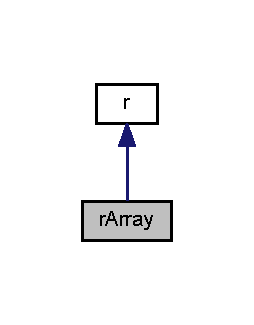
\includegraphics[width=122pt]{class_pierce_moore_1_1_ruby_p_h_p_1_1r_array__inherit__graph}
\end{center}
\end{figure}


Collaboration diagram for r\-Array\-:
\nopagebreak
\begin{figure}[H]
\begin{center}
\leavevmode
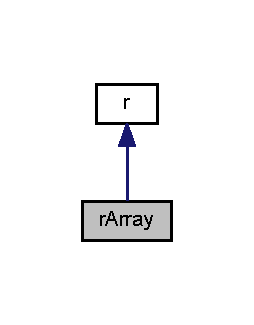
\includegraphics[width=122pt]{class_pierce_moore_1_1_ruby_p_h_p_1_1r_array__coll__graph}
\end{center}
\end{figure}
\subsection*{Public Member Functions}
\begin{DoxyCompactItemize}
\item 
\hyperlink{class_pierce_moore_1_1_ruby_p_h_p_1_1r_array_a4b0c1fe0e6c94ec2df5006f414b164c4}{\-\_\-\-\_\-construct} (\$item)
\item 
\hyperlink{class_pierce_moore_1_1_ruby_p_h_p_1_1r_array_a977f683ea39406f1243565b0ee28bd5a}{srt} (\$method= 'sort')
\item 
\hyperlink{class_pierce_moore_1_1_ruby_p_h_p_1_1r_array_a24a0a2d08214aa208efaf13be12b41fe}{push} (\$item, \$location=\char`\"{}end\char`\"{})
\item 
\hyperlink{class_pierce_moore_1_1_ruby_p_h_p_1_1r_array_a74e94d71195d9cbb9c9e3bca3353d912}{rotate} ()
\item 
\hyperlink{class_pierce_moore_1_1_ruby_p_h_p_1_1r_array_ace98c3b631ca27cdb027bbe389ef8628}{sample} (\$size=1)
\item 
\hyperlink{class_pierce_moore_1_1_ruby_p_h_p_1_1r_array_ae01473d9a4d7f2c33c1a157b9cce13f4}{slice} (\$start=0, \$\hyperlink{class_pierce_moore_1_1_ruby_p_h_p_1_1r_af7fc0f34bd91e802322d34f8942c3eee}{count}=null)
\item 
\hyperlink{class_pierce_moore_1_1_ruby_p_h_p_1_1r_array_a032c9d1b1b6ac32627b95225479aa7c0}{uniq} ()
\item 
\hyperlink{class_pierce_moore_1_1_ruby_p_h_p_1_1r_array_a2dba4fd3850e2c373dad4604d170dfa6}{zip} (\$args)
\item 
\hyperlink{class_pierce_moore_1_1_ruby_p_h_p_1_1r_array_a2108d0f07e9bca6160bf5885703de972}{to\-J\-S\-O\-N} ()
\item 
\hyperlink{class_pierce_moore_1_1_ruby_p_h_p_1_1r_array_ae456068dd57aa56c7fc891a526e67c32}{from\-J\-S\-O\-N} ()
\item 
\hyperlink{class_pierce_moore_1_1_ruby_p_h_p_1_1r_array_a20d848af138f92c4604f0bcecce267e2}{serial} ()
\item 
\hyperlink{class_pierce_moore_1_1_ruby_p_h_p_1_1r_array_a5664dc3d9f1d71ac463a833d37583e84}{unserial} ()
\item 
\hyperlink{class_pierce_moore_1_1_ruby_p_h_p_1_1r_array_ada723c8fc4c1599c3f0a5a73698ef7fd}{index} (\$key)
\item 
\hyperlink{class_pierce_moore_1_1_ruby_p_h_p_1_1r_array_a69c3762d52c367c08ca4dd234f5576df}{concat} (\$item, \$position=\char`\"{}end\char`\"{})
\item 
\hyperlink{class_pierce_moore_1_1_ruby_p_h_p_1_1r_array_a7e2ed8a2b96e8c0340390647f081557c}{prepend} (\$item)
\item 
\hyperlink{class_pierce_moore_1_1_ruby_p_h_p_1_1r_array_a61a8836731b261782082897b5fd9a841}{array\-Slash} (\$array, \$mode)
\item 
\hyperlink{class_pierce_moore_1_1_ruby_p_h_p_1_1r_array_a462c50b3bb38143adf421fe36bdc8cc5}{array\-Replace} (\$array, \$item, \$replacer)
\item 
\hyperlink{class_pierce_moore_1_1_ruby_p_h_p_1_1r_array_ae07220d820951c5ab6e43e05e325e552}{flatten} (\$\hyperlink{class_pierce_moore_1_1_ruby_p_h_p_1_1r_af745c1e6bc71ed38a120043c0cb13416}{val}=null, \$key=null)
\item 
\hyperlink{class_pierce_moore_1_1_ruby_p_h_p_1_1r_array_aa74a2edd6f3cbb5c5353f7faa97b6d70}{delete} (\$key)
\end{DoxyCompactItemize}
\subsection*{Protected Member Functions}
\begin{DoxyCompactItemize}
\item 
\hyperlink{class_pierce_moore_1_1_ruby_p_h_p_1_1r_array_a6308a44baf5a781ceb74550e7ea2cb25}{build\-Array} ()
\end{DoxyCompactItemize}


\subsection{Detailed Description}


Definition at line 13 of file class.\-array.\-rubyphp.\-php.



\subsection{Constructor \& Destructor Documentation}
\hypertarget{class_pierce_moore_1_1_ruby_p_h_p_1_1r_array_a4b0c1fe0e6c94ec2df5006f414b164c4}{\index{Pierce\-Moore\-::\-Ruby\-P\-H\-P\-::r\-Array@{Pierce\-Moore\-::\-Ruby\-P\-H\-P\-::r\-Array}!\-\_\-\-\_\-construct@{\-\_\-\-\_\-construct}}
\index{\-\_\-\-\_\-construct@{\-\_\-\-\_\-construct}!PierceMoore::RubyPHP::rArray@{Pierce\-Moore\-::\-Ruby\-P\-H\-P\-::r\-Array}}
\subsubsection[{\-\_\-\-\_\-construct}]{\setlength{\rightskip}{0pt plus 5cm}{\bf \-\_\-\-\_\-construct} (
\begin{DoxyParamCaption}
\item[{\$}]{item}
\end{DoxyParamCaption}
)}}\label{class_pierce_moore_1_1_ruby_p_h_p_1_1r_array_a4b0c1fe0e6c94ec2df5006f414b164c4}


Definition at line 15 of file class.\-array.\-rubyphp.\-php.



Here is the call graph for this function\-:
\nopagebreak
\begin{figure}[H]
\begin{center}
\leavevmode
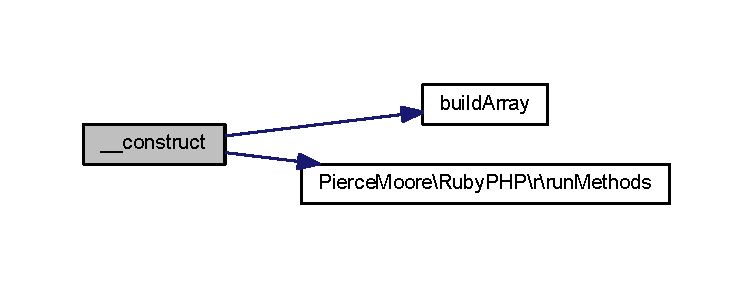
\includegraphics[width=350pt]{class_pierce_moore_1_1_ruby_p_h_p_1_1r_array_a4b0c1fe0e6c94ec2df5006f414b164c4_cgraph}
\end{center}
\end{figure}




\subsection{Member Function Documentation}
\hypertarget{class_pierce_moore_1_1_ruby_p_h_p_1_1r_array_a462c50b3bb38143adf421fe36bdc8cc5}{\index{Pierce\-Moore\-::\-Ruby\-P\-H\-P\-::r\-Array@{Pierce\-Moore\-::\-Ruby\-P\-H\-P\-::r\-Array}!array\-Replace@{array\-Replace}}
\index{array\-Replace@{array\-Replace}!PierceMoore::RubyPHP::rArray@{Pierce\-Moore\-::\-Ruby\-P\-H\-P\-::r\-Array}}
\subsubsection[{array\-Replace}]{\setlength{\rightskip}{0pt plus 5cm}{\bf array\-Replace} (
\begin{DoxyParamCaption}
\item[{\$}]{array, }
\item[{\$}]{item, }
\item[{\$}]{replacer}
\end{DoxyParamCaption}
)}}\label{class_pierce_moore_1_1_ruby_p_h_p_1_1r_array_a462c50b3bb38143adf421fe36bdc8cc5}

\begin{DoxyParams}[1]{Parameters}
array & {\em \$array} & -\/ The Haystack to search in \\
\hline
string & {\em \$item} & -\/ The pattern or key to match against (regex) \\
\hline
mixed & {\em \$replacer} & -\/ The item that will replace the found key \\
\hline
\end{DoxyParams}
\begin{DoxyReturn}{Returns}
mixed 
\end{DoxyReturn}


Definition at line 420 of file class.\-array.\-rubyphp.\-php.

\hypertarget{class_pierce_moore_1_1_ruby_p_h_p_1_1r_array_a61a8836731b261782082897b5fd9a841}{\index{Pierce\-Moore\-::\-Ruby\-P\-H\-P\-::r\-Array@{Pierce\-Moore\-::\-Ruby\-P\-H\-P\-::r\-Array}!array\-Slash@{array\-Slash}}
\index{array\-Slash@{array\-Slash}!PierceMoore::RubyPHP::rArray@{Pierce\-Moore\-::\-Ruby\-P\-H\-P\-::r\-Array}}
\subsubsection[{array\-Slash}]{\setlength{\rightskip}{0pt plus 5cm}{\bf array\-Slash} (
\begin{DoxyParamCaption}
\item[{\$}]{array, }
\item[{\$}]{mode}
\end{DoxyParamCaption}
)}}\label{class_pierce_moore_1_1_ruby_p_h_p_1_1r_array_a61a8836731b261782082897b5fd9a841}


Definition at line 396 of file class.\-array.\-rubyphp.\-php.



Here is the call graph for this function\-:
\nopagebreak
\begin{figure}[H]
\begin{center}
\leavevmode
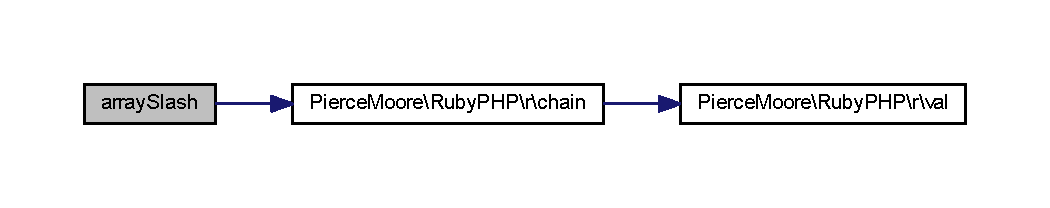
\includegraphics[width=350pt]{class_pierce_moore_1_1_ruby_p_h_p_1_1r_array_a61a8836731b261782082897b5fd9a841_cgraph}
\end{center}
\end{figure}


\hypertarget{class_pierce_moore_1_1_ruby_p_h_p_1_1r_array_a6308a44baf5a781ceb74550e7ea2cb25}{\index{Pierce\-Moore\-::\-Ruby\-P\-H\-P\-::r\-Array@{Pierce\-Moore\-::\-Ruby\-P\-H\-P\-::r\-Array}!build\-Array@{build\-Array}}
\index{build\-Array@{build\-Array}!PierceMoore::RubyPHP::rArray@{Pierce\-Moore\-::\-Ruby\-P\-H\-P\-::r\-Array}}
\subsubsection[{build\-Array}]{\setlength{\rightskip}{0pt plus 5cm}{\bf build\-Array} (
\begin{DoxyParamCaption}
{}
\end{DoxyParamCaption}
)\hspace{0.3cm}{\ttfamily  \mbox{[}protected\mbox{]}}}}\label{class_pierce_moore_1_1_ruby_p_h_p_1_1r_array_a6308a44baf5a781ceb74550e7ea2cb25}
\begin{DoxyReturn}{Returns}
boolean 
\end{DoxyReturn}


Definition at line 29 of file class.\-array.\-rubyphp.\-php.



Here is the caller graph for this function\-:
\nopagebreak
\begin{figure}[H]
\begin{center}
\leavevmode
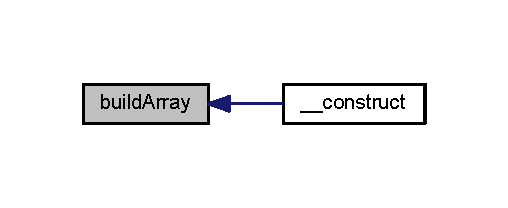
\includegraphics[width=244pt]{class_pierce_moore_1_1_ruby_p_h_p_1_1r_array_a6308a44baf5a781ceb74550e7ea2cb25_icgraph}
\end{center}
\end{figure}


\hypertarget{class_pierce_moore_1_1_ruby_p_h_p_1_1r_array_a69c3762d52c367c08ca4dd234f5576df}{\index{Pierce\-Moore\-::\-Ruby\-P\-H\-P\-::r\-Array@{Pierce\-Moore\-::\-Ruby\-P\-H\-P\-::r\-Array}!concat@{concat}}
\index{concat@{concat}!PierceMoore::RubyPHP::rArray@{Pierce\-Moore\-::\-Ruby\-P\-H\-P\-::r\-Array}}
\subsubsection[{concat}]{\setlength{\rightskip}{0pt plus 5cm}{\bf concat} (
\begin{DoxyParamCaption}
\item[{\$}]{item, }
\item[{\$}]{position = {\ttfamily \char`\"{}end\char`\"{}}}
\end{DoxyParamCaption}
)}}\label{class_pierce_moore_1_1_ruby_p_h_p_1_1r_array_a69c3762d52c367c08ca4dd234f5576df}

\begin{DoxyParams}[1]{Parameters}
mixed & {\em \$item} & -\/ The item that you would like appended to the object value array. Preferred\-: Array \\
\hline
string & {\em \$position} & -\/ The position in the array you would like the value appended. Accepts \char`\"{}start\char`\"{} \char`\"{}fin\char`\"{} \char`\"{}begin\char`\"{} and \char`\"{}end\char`\"{} \\
\hline
\end{DoxyParams}
\begin{DoxyReturn}{Returns}
mixed 
\end{DoxyReturn}


Definition at line 332 of file class.\-array.\-rubyphp.\-php.



Here is the call graph for this function\-:
\nopagebreak
\begin{figure}[H]
\begin{center}
\leavevmode
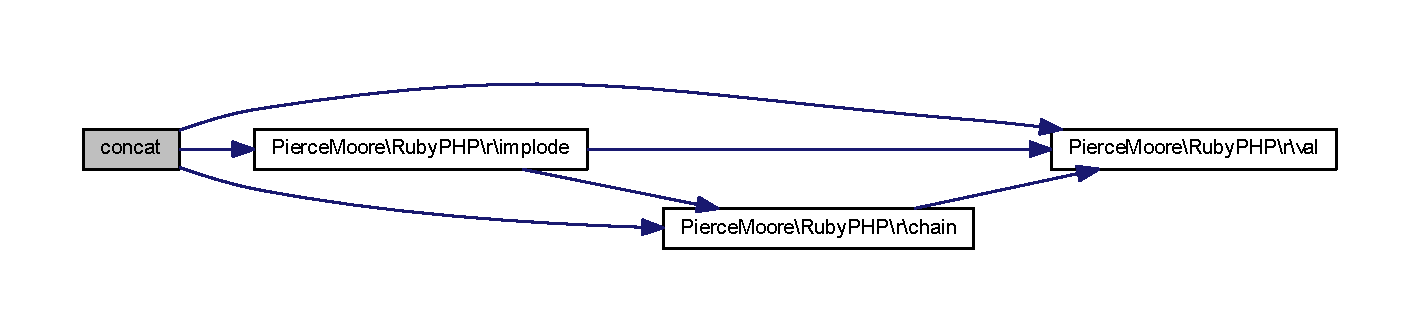
\includegraphics[width=350pt]{class_pierce_moore_1_1_ruby_p_h_p_1_1r_array_a69c3762d52c367c08ca4dd234f5576df_cgraph}
\end{center}
\end{figure}


\hypertarget{class_pierce_moore_1_1_ruby_p_h_p_1_1r_array_aa74a2edd6f3cbb5c5353f7faa97b6d70}{\index{Pierce\-Moore\-::\-Ruby\-P\-H\-P\-::r\-Array@{Pierce\-Moore\-::\-Ruby\-P\-H\-P\-::r\-Array}!delete@{delete}}
\index{delete@{delete}!PierceMoore::RubyPHP::rArray@{Pierce\-Moore\-::\-Ruby\-P\-H\-P\-::r\-Array}}
\subsubsection[{delete}]{\setlength{\rightskip}{0pt plus 5cm}{\bf delete} (
\begin{DoxyParamCaption}
\item[{\$}]{key}
\end{DoxyParamCaption}
)}}\label{class_pierce_moore_1_1_ruby_p_h_p_1_1r_array_aa74a2edd6f3cbb5c5353f7faa97b6d70}


Definition at line 478 of file class.\-array.\-rubyphp.\-php.



Here is the call graph for this function\-:
\nopagebreak
\begin{figure}[H]
\begin{center}
\leavevmode
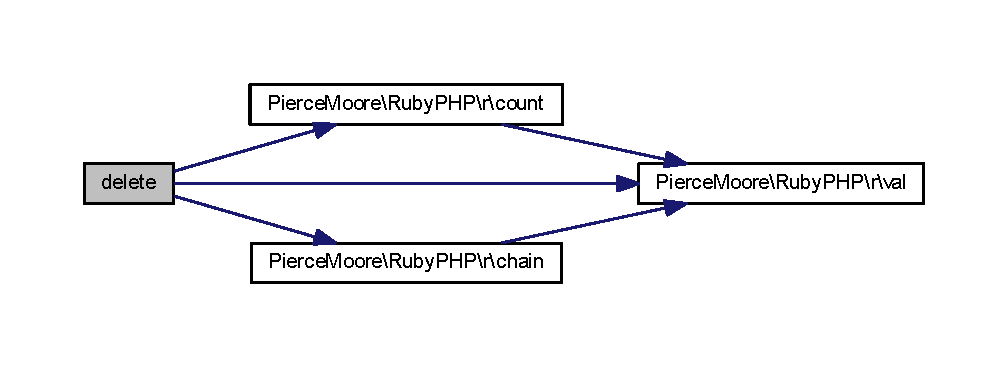
\includegraphics[width=350pt]{class_pierce_moore_1_1_ruby_p_h_p_1_1r_array_aa74a2edd6f3cbb5c5353f7faa97b6d70_cgraph}
\end{center}
\end{figure}


\hypertarget{class_pierce_moore_1_1_ruby_p_h_p_1_1r_array_ae07220d820951c5ab6e43e05e325e552}{\index{Pierce\-Moore\-::\-Ruby\-P\-H\-P\-::r\-Array@{Pierce\-Moore\-::\-Ruby\-P\-H\-P\-::r\-Array}!flatten@{flatten}}
\index{flatten@{flatten}!PierceMoore::RubyPHP::rArray@{Pierce\-Moore\-::\-Ruby\-P\-H\-P\-::r\-Array}}
\subsubsection[{flatten}]{\setlength{\rightskip}{0pt plus 5cm}{\bf flatten} (
\begin{DoxyParamCaption}
\item[{\$}]{val = {\ttfamily null}, }
\item[{\$}]{key = {\ttfamily null}}
\end{DoxyParamCaption}
)}}\label{class_pierce_moore_1_1_ruby_p_h_p_1_1r_array_ae07220d820951c5ab6e43e05e325e552}

\begin{DoxyParams}[1]{Parameters}
mixed & {\em \$val} & -\/ The value of the flattened keypair \\
\hline
mixed & {\em \$key} & -\/ The key of the flattened keypair \\
\hline
\end{DoxyParams}
\begin{DoxyReturn}{Returns}
array 
\end{DoxyReturn}


Definition at line 457 of file class.\-array.\-rubyphp.\-php.



Here is the call graph for this function\-:
\nopagebreak
\begin{figure}[H]
\begin{center}
\leavevmode
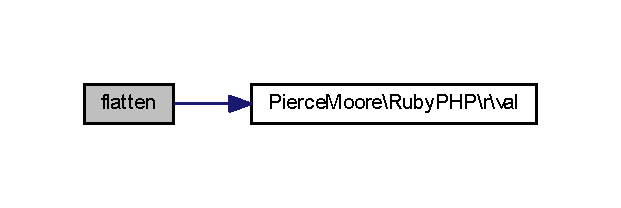
\includegraphics[width=298pt]{class_pierce_moore_1_1_ruby_p_h_p_1_1r_array_ae07220d820951c5ab6e43e05e325e552_cgraph}
\end{center}
\end{figure}


\hypertarget{class_pierce_moore_1_1_ruby_p_h_p_1_1r_array_ae456068dd57aa56c7fc891a526e67c32}{\index{Pierce\-Moore\-::\-Ruby\-P\-H\-P\-::r\-Array@{Pierce\-Moore\-::\-Ruby\-P\-H\-P\-::r\-Array}!from\-J\-S\-O\-N@{from\-J\-S\-O\-N}}
\index{from\-J\-S\-O\-N@{from\-J\-S\-O\-N}!PierceMoore::RubyPHP::rArray@{Pierce\-Moore\-::\-Ruby\-P\-H\-P\-::r\-Array}}
\subsubsection[{from\-J\-S\-O\-N}]{\setlength{\rightskip}{0pt plus 5cm}{\bf from\-J\-S\-O\-N} (
\begin{DoxyParamCaption}
{}
\end{DoxyParamCaption}
)}}\label{class_pierce_moore_1_1_ruby_p_h_p_1_1r_array_ae456068dd57aa56c7fc891a526e67c32}
\begin{DoxyReturn}{Returns}
string 
\end{DoxyReturn}


Definition at line 267 of file class.\-array.\-rubyphp.\-php.



Here is the call graph for this function\-:
\nopagebreak
\begin{figure}[H]
\begin{center}
\leavevmode
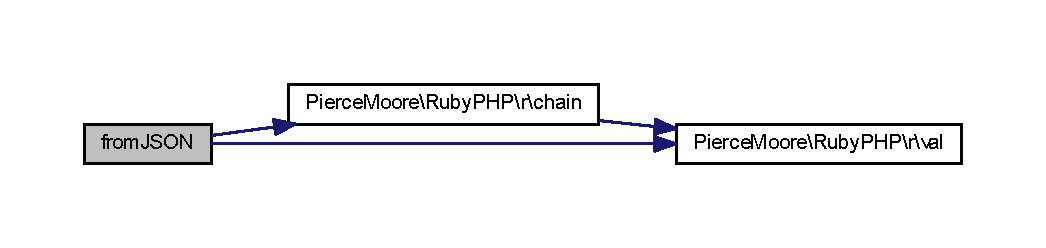
\includegraphics[width=350pt]{class_pierce_moore_1_1_ruby_p_h_p_1_1r_array_ae456068dd57aa56c7fc891a526e67c32_cgraph}
\end{center}
\end{figure}


\hypertarget{class_pierce_moore_1_1_ruby_p_h_p_1_1r_array_ada723c8fc4c1599c3f0a5a73698ef7fd}{\index{Pierce\-Moore\-::\-Ruby\-P\-H\-P\-::r\-Array@{Pierce\-Moore\-::\-Ruby\-P\-H\-P\-::r\-Array}!index@{index}}
\index{index@{index}!PierceMoore::RubyPHP::rArray@{Pierce\-Moore\-::\-Ruby\-P\-H\-P\-::r\-Array}}
\subsubsection[{index}]{\setlength{\rightskip}{0pt plus 5cm}{\bf index} (
\begin{DoxyParamCaption}
\item[{\$}]{key}
\end{DoxyParamCaption}
)}}\label{class_pierce_moore_1_1_ruby_p_h_p_1_1r_array_ada723c8fc4c1599c3f0a5a73698ef7fd}

\begin{DoxyParams}[1]{Parameters}
int & {\em \$key} & -\/ The key to locate \\
\hline
\end{DoxyParams}
\begin{DoxyReturn}{Returns}
mixed 
\end{DoxyReturn}


Definition at line 310 of file class.\-array.\-rubyphp.\-php.



Here is the call graph for this function\-:
\nopagebreak
\begin{figure}[H]
\begin{center}
\leavevmode
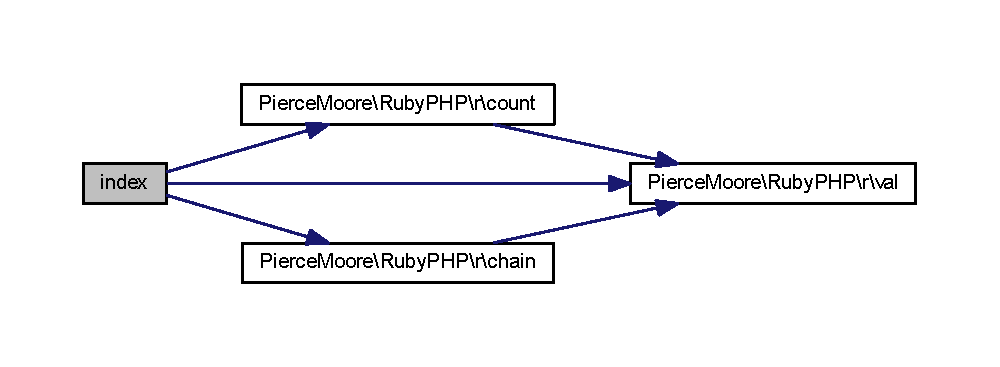
\includegraphics[width=350pt]{class_pierce_moore_1_1_ruby_p_h_p_1_1r_array_ada723c8fc4c1599c3f0a5a73698ef7fd_cgraph}
\end{center}
\end{figure}


\hypertarget{class_pierce_moore_1_1_ruby_p_h_p_1_1r_array_a7e2ed8a2b96e8c0340390647f081557c}{\index{Pierce\-Moore\-::\-Ruby\-P\-H\-P\-::r\-Array@{Pierce\-Moore\-::\-Ruby\-P\-H\-P\-::r\-Array}!prepend@{prepend}}
\index{prepend@{prepend}!PierceMoore::RubyPHP::rArray@{Pierce\-Moore\-::\-Ruby\-P\-H\-P\-::r\-Array}}
\subsubsection[{prepend}]{\setlength{\rightskip}{0pt plus 5cm}{\bf prepend} (
\begin{DoxyParamCaption}
\item[{\$}]{item}
\end{DoxyParamCaption}
)}}\label{class_pierce_moore_1_1_ruby_p_h_p_1_1r_array_a7e2ed8a2b96e8c0340390647f081557c}

\begin{DoxyParams}[1]{Parameters}
mixed & {\em \$item} & -\/ The item to be prepended to the existing array \\
\hline
\end{DoxyParams}
\begin{DoxyReturn}{Returns}
mixed 
\end{DoxyReturn}


Definition at line 371 of file class.\-array.\-rubyphp.\-php.



Here is the call graph for this function\-:
\nopagebreak
\begin{figure}[H]
\begin{center}
\leavevmode
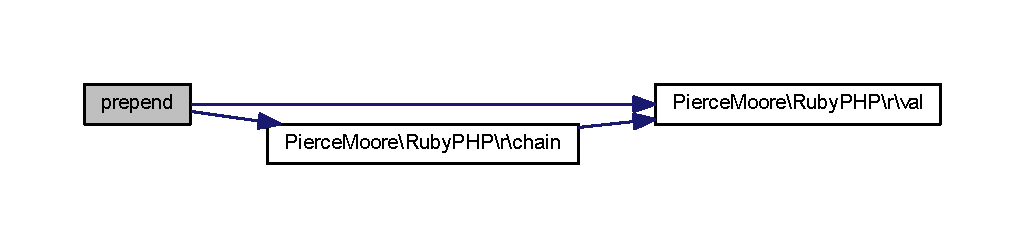
\includegraphics[width=350pt]{class_pierce_moore_1_1_ruby_p_h_p_1_1r_array_a7e2ed8a2b96e8c0340390647f081557c_cgraph}
\end{center}
\end{figure}


\hypertarget{class_pierce_moore_1_1_ruby_p_h_p_1_1r_array_a24a0a2d08214aa208efaf13be12b41fe}{\index{Pierce\-Moore\-::\-Ruby\-P\-H\-P\-::r\-Array@{Pierce\-Moore\-::\-Ruby\-P\-H\-P\-::r\-Array}!push@{push}}
\index{push@{push}!PierceMoore::RubyPHP::rArray@{Pierce\-Moore\-::\-Ruby\-P\-H\-P\-::r\-Array}}
\subsubsection[{push}]{\setlength{\rightskip}{0pt plus 5cm}{\bf push} (
\begin{DoxyParamCaption}
\item[{\$}]{item, }
\item[{\$}]{location = {\ttfamily \char`\"{}end\char`\"{}}}
\end{DoxyParamCaption}
)}}\label{class_pierce_moore_1_1_ruby_p_h_p_1_1r_array_a24a0a2d08214aa208efaf13be12b41fe}

\begin{DoxyParams}[1]{Parameters}
mixed & {\em \$item} & -\/ The item to be placed into the array \\
\hline
string & {\em \$location} & -\/ The item to be \\
\hline
\end{DoxyParams}
\begin{DoxyReturn}{Returns}
mixed 
\end{DoxyReturn}


Definition at line 62 of file class.\-array.\-rubyphp.\-php.



Here is the call graph for this function\-:
\nopagebreak
\begin{figure}[H]
\begin{center}
\leavevmode
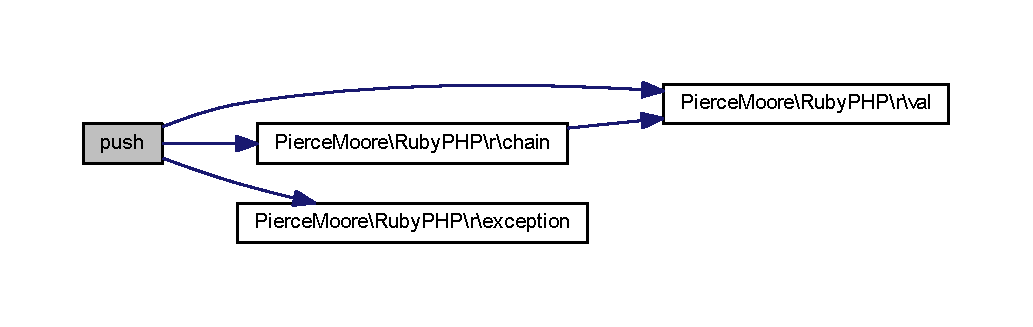
\includegraphics[width=350pt]{class_pierce_moore_1_1_ruby_p_h_p_1_1r_array_a24a0a2d08214aa208efaf13be12b41fe_cgraph}
\end{center}
\end{figure}


\hypertarget{class_pierce_moore_1_1_ruby_p_h_p_1_1r_array_a74e94d71195d9cbb9c9e3bca3353d912}{\index{Pierce\-Moore\-::\-Ruby\-P\-H\-P\-::r\-Array@{Pierce\-Moore\-::\-Ruby\-P\-H\-P\-::r\-Array}!rotate@{rotate}}
\index{rotate@{rotate}!PierceMoore::RubyPHP::rArray@{Pierce\-Moore\-::\-Ruby\-P\-H\-P\-::r\-Array}}
\subsubsection[{rotate}]{\setlength{\rightskip}{0pt plus 5cm}{\bf rotate} (
\begin{DoxyParamCaption}
{}
\end{DoxyParamCaption}
)}}\label{class_pierce_moore_1_1_ruby_p_h_p_1_1r_array_a74e94d71195d9cbb9c9e3bca3353d912}
\begin{DoxyReturn}{Returns}
array 
\end{DoxyReturn}


Definition at line 98 of file class.\-array.\-rubyphp.\-php.



Here is the call graph for this function\-:
\nopagebreak
\begin{figure}[H]
\begin{center}
\leavevmode
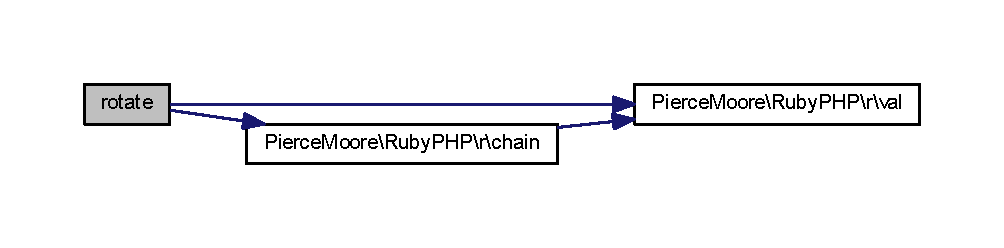
\includegraphics[width=350pt]{class_pierce_moore_1_1_ruby_p_h_p_1_1r_array_a74e94d71195d9cbb9c9e3bca3353d912_cgraph}
\end{center}
\end{figure}


\hypertarget{class_pierce_moore_1_1_ruby_p_h_p_1_1r_array_ace98c3b631ca27cdb027bbe389ef8628}{\index{Pierce\-Moore\-::\-Ruby\-P\-H\-P\-::r\-Array@{Pierce\-Moore\-::\-Ruby\-P\-H\-P\-::r\-Array}!sample@{sample}}
\index{sample@{sample}!PierceMoore::RubyPHP::rArray@{Pierce\-Moore\-::\-Ruby\-P\-H\-P\-::r\-Array}}
\subsubsection[{sample}]{\setlength{\rightskip}{0pt plus 5cm}{\bf sample} (
\begin{DoxyParamCaption}
\item[{\$}]{size = {\ttfamily 1}}
\end{DoxyParamCaption}
)}}\label{class_pierce_moore_1_1_ruby_p_h_p_1_1r_array_ace98c3b631ca27cdb027bbe389ef8628}

\begin{DoxyParams}[1]{Parameters}
int & {\em \$size} & -\/ The number of random elements to return. \\
\hline
\end{DoxyParams}
\begin{DoxyReturn}{Returns}
mixed 
\end{DoxyReturn}


Definition at line 116 of file class.\-array.\-rubyphp.\-php.



Here is the call graph for this function\-:
\nopagebreak
\begin{figure}[H]
\begin{center}
\leavevmode
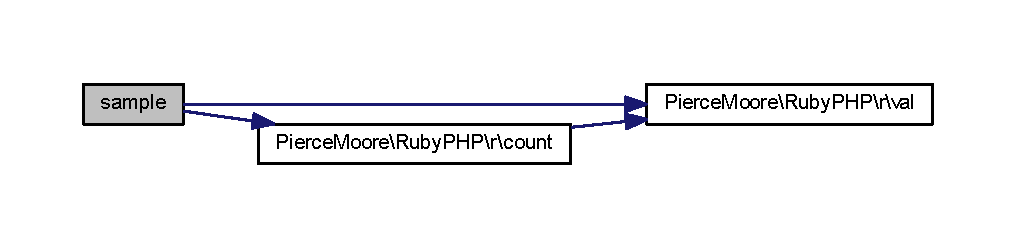
\includegraphics[width=350pt]{class_pierce_moore_1_1_ruby_p_h_p_1_1r_array_ace98c3b631ca27cdb027bbe389ef8628_cgraph}
\end{center}
\end{figure}


\hypertarget{class_pierce_moore_1_1_ruby_p_h_p_1_1r_array_a20d848af138f92c4604f0bcecce267e2}{\index{Pierce\-Moore\-::\-Ruby\-P\-H\-P\-::r\-Array@{Pierce\-Moore\-::\-Ruby\-P\-H\-P\-::r\-Array}!serial@{serial}}
\index{serial@{serial}!PierceMoore::RubyPHP::rArray@{Pierce\-Moore\-::\-Ruby\-P\-H\-P\-::r\-Array}}
\subsubsection[{serial}]{\setlength{\rightskip}{0pt plus 5cm}{\bf serial} (
\begin{DoxyParamCaption}
{}
\end{DoxyParamCaption}
)}}\label{class_pierce_moore_1_1_ruby_p_h_p_1_1r_array_a20d848af138f92c4604f0bcecce267e2}
\begin{DoxyReturn}{Returns}
string 
\end{DoxyReturn}


Definition at line 281 of file class.\-array.\-rubyphp.\-php.



Here is the call graph for this function\-:
\nopagebreak
\begin{figure}[H]
\begin{center}
\leavevmode
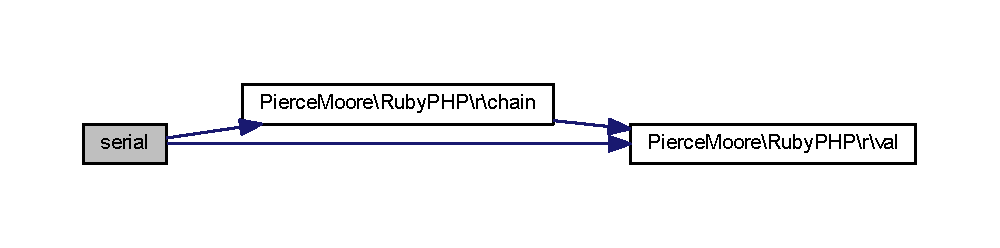
\includegraphics[width=350pt]{class_pierce_moore_1_1_ruby_p_h_p_1_1r_array_a20d848af138f92c4604f0bcecce267e2_cgraph}
\end{center}
\end{figure}


\hypertarget{class_pierce_moore_1_1_ruby_p_h_p_1_1r_array_ae01473d9a4d7f2c33c1a157b9cce13f4}{\index{Pierce\-Moore\-::\-Ruby\-P\-H\-P\-::r\-Array@{Pierce\-Moore\-::\-Ruby\-P\-H\-P\-::r\-Array}!slice@{slice}}
\index{slice@{slice}!PierceMoore::RubyPHP::rArray@{Pierce\-Moore\-::\-Ruby\-P\-H\-P\-::r\-Array}}
\subsubsection[{slice}]{\setlength{\rightskip}{0pt plus 5cm}{\bf slice} (
\begin{DoxyParamCaption}
\item[{\$}]{start = {\ttfamily 0}, }
\item[{\$}]{count = {\ttfamily null}}
\end{DoxyParamCaption}
)}}\label{class_pierce_moore_1_1_ruby_p_h_p_1_1r_array_ae01473d9a4d7f2c33c1a157b9cce13f4}

\begin{DoxyParams}[1]{Parameters}
int & {\em \$start} & -\/ The starting index of the slice \\
\hline
int & {\em \$count} & -\/ The size of the slice. \\
\hline
\end{DoxyParams}
\begin{DoxyReturn}{Returns}
mixed 
\end{DoxyReturn}


Definition at line 150 of file class.\-array.\-rubyphp.\-php.



Here is the call graph for this function\-:
\nopagebreak
\begin{figure}[H]
\begin{center}
\leavevmode
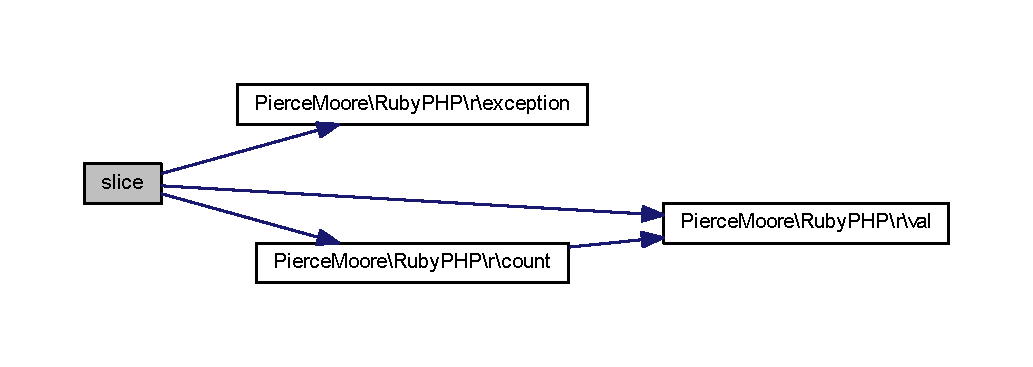
\includegraphics[width=350pt]{class_pierce_moore_1_1_ruby_p_h_p_1_1r_array_ae01473d9a4d7f2c33c1a157b9cce13f4_cgraph}
\end{center}
\end{figure}


\hypertarget{class_pierce_moore_1_1_ruby_p_h_p_1_1r_array_a977f683ea39406f1243565b0ee28bd5a}{\index{Pierce\-Moore\-::\-Ruby\-P\-H\-P\-::r\-Array@{Pierce\-Moore\-::\-Ruby\-P\-H\-P\-::r\-Array}!srt@{srt}}
\index{srt@{srt}!PierceMoore::RubyPHP::rArray@{Pierce\-Moore\-::\-Ruby\-P\-H\-P\-::r\-Array}}
\subsubsection[{srt}]{\setlength{\rightskip}{0pt plus 5cm}{\bf srt} (
\begin{DoxyParamCaption}
\item[{\$}]{method = {\ttfamily 'sort'}}
\end{DoxyParamCaption}
)}}\label{class_pierce_moore_1_1_ruby_p_h_p_1_1r_array_a977f683ea39406f1243565b0ee28bd5a}
\begin{DoxyReturn}{Returns}
mixed 
\end{DoxyReturn}


Definition at line 43 of file class.\-array.\-rubyphp.\-php.



Here is the call graph for this function\-:
\nopagebreak
\begin{figure}[H]
\begin{center}
\leavevmode
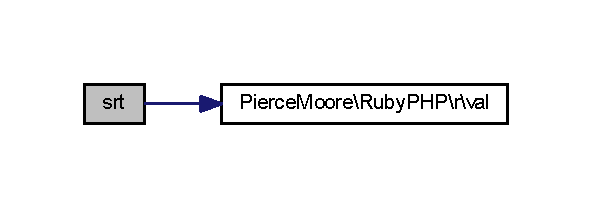
\includegraphics[width=284pt]{class_pierce_moore_1_1_ruby_p_h_p_1_1r_array_a977f683ea39406f1243565b0ee28bd5a_cgraph}
\end{center}
\end{figure}


\hypertarget{class_pierce_moore_1_1_ruby_p_h_p_1_1r_array_a2108d0f07e9bca6160bf5885703de972}{\index{Pierce\-Moore\-::\-Ruby\-P\-H\-P\-::r\-Array@{Pierce\-Moore\-::\-Ruby\-P\-H\-P\-::r\-Array}!to\-J\-S\-O\-N@{to\-J\-S\-O\-N}}
\index{to\-J\-S\-O\-N@{to\-J\-S\-O\-N}!PierceMoore::RubyPHP::rArray@{Pierce\-Moore\-::\-Ruby\-P\-H\-P\-::r\-Array}}
\subsubsection[{to\-J\-S\-O\-N}]{\setlength{\rightskip}{0pt plus 5cm}{\bf to\-J\-S\-O\-N} (
\begin{DoxyParamCaption}
{}
\end{DoxyParamCaption}
)}}\label{class_pierce_moore_1_1_ruby_p_h_p_1_1r_array_a2108d0f07e9bca6160bf5885703de972}
\begin{DoxyReturn}{Returns}
string 
\end{DoxyReturn}


Definition at line 253 of file class.\-array.\-rubyphp.\-php.



Here is the call graph for this function\-:
\nopagebreak
\begin{figure}[H]
\begin{center}
\leavevmode
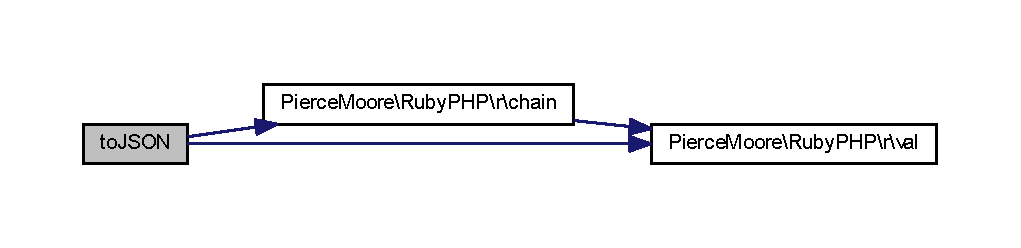
\includegraphics[width=350pt]{class_pierce_moore_1_1_ruby_p_h_p_1_1r_array_a2108d0f07e9bca6160bf5885703de972_cgraph}
\end{center}
\end{figure}


\hypertarget{class_pierce_moore_1_1_ruby_p_h_p_1_1r_array_a032c9d1b1b6ac32627b95225479aa7c0}{\index{Pierce\-Moore\-::\-Ruby\-P\-H\-P\-::r\-Array@{Pierce\-Moore\-::\-Ruby\-P\-H\-P\-::r\-Array}!uniq@{uniq}}
\index{uniq@{uniq}!PierceMoore::RubyPHP::rArray@{Pierce\-Moore\-::\-Ruby\-P\-H\-P\-::r\-Array}}
\subsubsection[{uniq}]{\setlength{\rightskip}{0pt plus 5cm}{\bf uniq} (
\begin{DoxyParamCaption}
{}
\end{DoxyParamCaption}
)}}\label{class_pierce_moore_1_1_ruby_p_h_p_1_1r_array_a032c9d1b1b6ac32627b95225479aa7c0}
\begin{DoxyReturn}{Returns}
mixed 
\end{DoxyReturn}


Definition at line 189 of file class.\-array.\-rubyphp.\-php.



Here is the call graph for this function\-:
\nopagebreak
\begin{figure}[H]
\begin{center}
\leavevmode
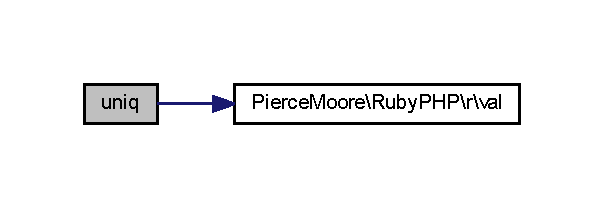
\includegraphics[width=290pt]{class_pierce_moore_1_1_ruby_p_h_p_1_1r_array_a032c9d1b1b6ac32627b95225479aa7c0_cgraph}
\end{center}
\end{figure}


\hypertarget{class_pierce_moore_1_1_ruby_p_h_p_1_1r_array_a5664dc3d9f1d71ac463a833d37583e84}{\index{Pierce\-Moore\-::\-Ruby\-P\-H\-P\-::r\-Array@{Pierce\-Moore\-::\-Ruby\-P\-H\-P\-::r\-Array}!unserial@{unserial}}
\index{unserial@{unserial}!PierceMoore::RubyPHP::rArray@{Pierce\-Moore\-::\-Ruby\-P\-H\-P\-::r\-Array}}
\subsubsection[{unserial}]{\setlength{\rightskip}{0pt plus 5cm}{\bf unserial} (
\begin{DoxyParamCaption}
{}
\end{DoxyParamCaption}
)}}\label{class_pierce_moore_1_1_ruby_p_h_p_1_1r_array_a5664dc3d9f1d71ac463a833d37583e84}
\begin{DoxyReturn}{Returns}
mixed 
\end{DoxyReturn}


Definition at line 295 of file class.\-array.\-rubyphp.\-php.



Here is the call graph for this function\-:
\nopagebreak
\begin{figure}[H]
\begin{center}
\leavevmode
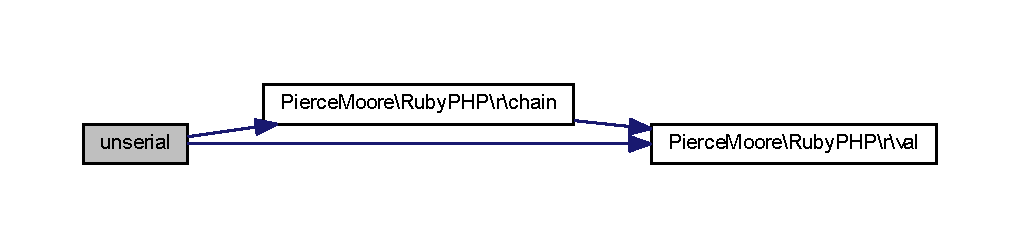
\includegraphics[width=350pt]{class_pierce_moore_1_1_ruby_p_h_p_1_1r_array_a5664dc3d9f1d71ac463a833d37583e84_cgraph}
\end{center}
\end{figure}


\hypertarget{class_pierce_moore_1_1_ruby_p_h_p_1_1r_array_a2dba4fd3850e2c373dad4604d170dfa6}{\index{Pierce\-Moore\-::\-Ruby\-P\-H\-P\-::r\-Array@{Pierce\-Moore\-::\-Ruby\-P\-H\-P\-::r\-Array}!zip@{zip}}
\index{zip@{zip}!PierceMoore::RubyPHP::rArray@{Pierce\-Moore\-::\-Ruby\-P\-H\-P\-::r\-Array}}
\subsubsection[{zip}]{\setlength{\rightskip}{0pt plus 5cm}{\bf zip} (
\begin{DoxyParamCaption}
\item[{\$}]{args}
\end{DoxyParamCaption}
)}}\label{class_pierce_moore_1_1_ruby_p_h_p_1_1r_array_a2dba4fd3850e2c373dad4604d170dfa6}
\begin{DoxyRefDesc}{Todo}
\item[\hyperlink{todo__todo000001}{Todo}]Check to see if array\-\_\-map() is more effective here than the solution I found. \end{DoxyRefDesc}

\begin{DoxyParams}[1]{Parameters}
mixed & {\em \$args} & -\/ This function accepts as many arguments as you throw at it. It will hard-\/typecast all arguments into arrays and go from there. \\
\hline
\end{DoxyParams}
\begin{DoxyReturn}{Returns}
mixed 
\end{DoxyReturn}


Definition at line 215 of file class.\-array.\-rubyphp.\-php.



Here is the call graph for this function\-:
\nopagebreak
\begin{figure}[H]
\begin{center}
\leavevmode
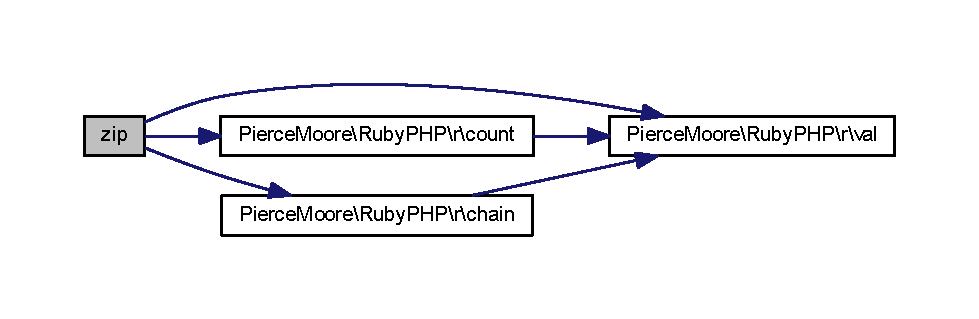
\includegraphics[width=350pt]{class_pierce_moore_1_1_ruby_p_h_p_1_1r_array_a2dba4fd3850e2c373dad4604d170dfa6_cgraph}
\end{center}
\end{figure}




The documentation for this class was generated from the following file\-:\begin{DoxyCompactItemize}
\item 
Ruby\-P\-H\-P/includes/\hyperlink{class_8array_8rubyphp_8php}{class.\-array.\-rubyphp.\-php}\end{DoxyCompactItemize}

\hypertarget{class_pierce_moore_1_1_ruby_p_h_p_1_1r_boolean}{\section{r\-Boolean Class Reference}
\label{class_pierce_moore_1_1_ruby_p_h_p_1_1r_boolean}\index{r\-Boolean@{r\-Boolean}}
}


Inheritance diagram for r\-Boolean\-:
\nopagebreak
\begin{figure}[H]
\begin{center}
\leavevmode
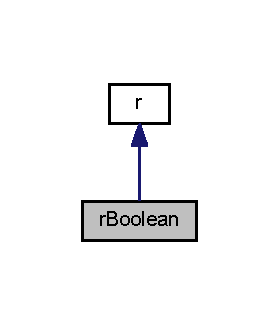
\includegraphics[width=134pt]{class_pierce_moore_1_1_ruby_p_h_p_1_1r_boolean__inherit__graph}
\end{center}
\end{figure}


Collaboration diagram for r\-Boolean\-:
\nopagebreak
\begin{figure}[H]
\begin{center}
\leavevmode
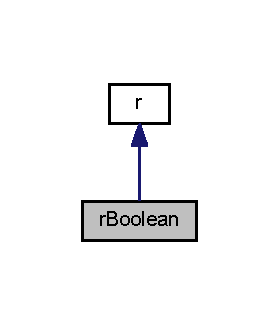
\includegraphics[width=134pt]{class_pierce_moore_1_1_ruby_p_h_p_1_1r_boolean__coll__graph}
\end{center}
\end{figure}
\subsection*{Public Member Functions}
\begin{DoxyCompactItemize}
\item 
\hyperlink{class_pierce_moore_1_1_ruby_p_h_p_1_1r_boolean_a4b0c1fe0e6c94ec2df5006f414b164c4}{\-\_\-\-\_\-construct} (\$item)
\end{DoxyCompactItemize}
\subsection*{Protected Member Functions}
\begin{DoxyCompactItemize}
\item 
\hyperlink{class_pierce_moore_1_1_ruby_p_h_p_1_1r_boolean_a48cb6ad2536902b3b8a316cee5933abc}{build\-Boolean} ()
\end{DoxyCompactItemize}


\subsection{Detailed Description}


Definition at line 13 of file class.\-boolean.\-rubyphp.\-php.



\subsection{Constructor \& Destructor Documentation}
\hypertarget{class_pierce_moore_1_1_ruby_p_h_p_1_1r_boolean_a4b0c1fe0e6c94ec2df5006f414b164c4}{\index{Pierce\-Moore\-::\-Ruby\-P\-H\-P\-::r\-Boolean@{Pierce\-Moore\-::\-Ruby\-P\-H\-P\-::r\-Boolean}!\-\_\-\-\_\-construct@{\-\_\-\-\_\-construct}}
\index{\-\_\-\-\_\-construct@{\-\_\-\-\_\-construct}!PierceMoore::RubyPHP::rBoolean@{Pierce\-Moore\-::\-Ruby\-P\-H\-P\-::r\-Boolean}}
\subsubsection[{\-\_\-\-\_\-construct}]{\setlength{\rightskip}{0pt plus 5cm}{\bf \-\_\-\-\_\-construct} (
\begin{DoxyParamCaption}
\item[{\$}]{item}
\end{DoxyParamCaption}
)}}\label{class_pierce_moore_1_1_ruby_p_h_p_1_1r_boolean_a4b0c1fe0e6c94ec2df5006f414b164c4}


Definition at line 15 of file class.\-boolean.\-rubyphp.\-php.



Here is the call graph for this function\-:
\nopagebreak
\begin{figure}[H]
\begin{center}
\leavevmode
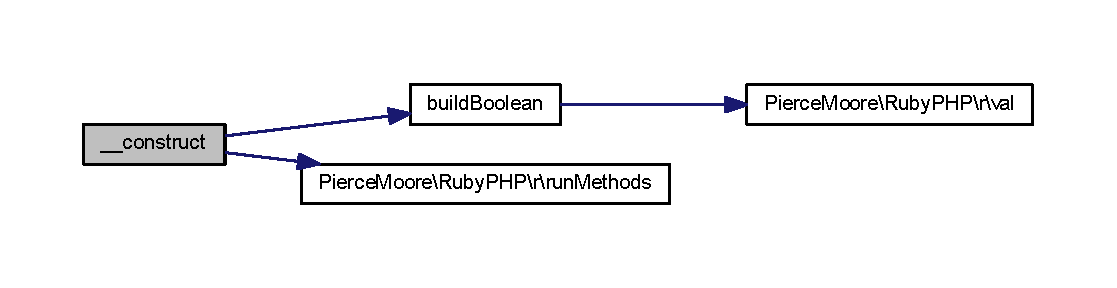
\includegraphics[width=350pt]{class_pierce_moore_1_1_ruby_p_h_p_1_1r_boolean_a4b0c1fe0e6c94ec2df5006f414b164c4_cgraph}
\end{center}
\end{figure}




\subsection{Member Function Documentation}
\hypertarget{class_pierce_moore_1_1_ruby_p_h_p_1_1r_boolean_a48cb6ad2536902b3b8a316cee5933abc}{\index{Pierce\-Moore\-::\-Ruby\-P\-H\-P\-::r\-Boolean@{Pierce\-Moore\-::\-Ruby\-P\-H\-P\-::r\-Boolean}!build\-Boolean@{build\-Boolean}}
\index{build\-Boolean@{build\-Boolean}!PierceMoore::RubyPHP::rBoolean@{Pierce\-Moore\-::\-Ruby\-P\-H\-P\-::r\-Boolean}}
\subsubsection[{build\-Boolean}]{\setlength{\rightskip}{0pt plus 5cm}{\bf build\-Boolean} (
\begin{DoxyParamCaption}
{}
\end{DoxyParamCaption}
)\hspace{0.3cm}{\ttfamily  \mbox{[}protected\mbox{]}}}}\label{class_pierce_moore_1_1_ruby_p_h_p_1_1r_boolean_a48cb6ad2536902b3b8a316cee5933abc}
\begin{DoxyReturn}{Returns}
boolean 
\end{DoxyReturn}


Definition at line 29 of file class.\-boolean.\-rubyphp.\-php.



Here is the call graph for this function\-:
\nopagebreak
\begin{figure}[H]
\begin{center}
\leavevmode
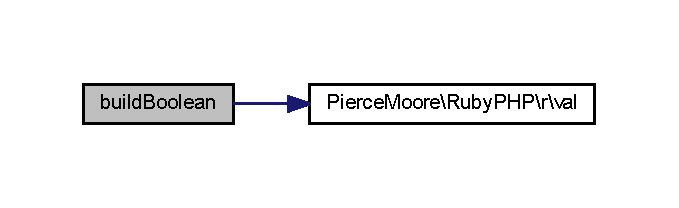
\includegraphics[width=326pt]{class_pierce_moore_1_1_ruby_p_h_p_1_1r_boolean_a48cb6ad2536902b3b8a316cee5933abc_cgraph}
\end{center}
\end{figure}




Here is the caller graph for this function\-:
\nopagebreak
\begin{figure}[H]
\begin{center}
\leavevmode
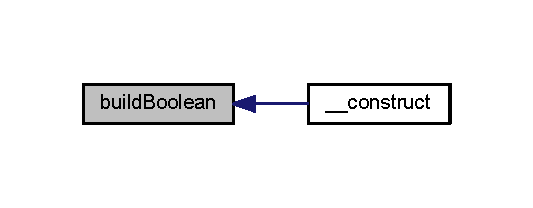
\includegraphics[width=256pt]{class_pierce_moore_1_1_ruby_p_h_p_1_1r_boolean_a48cb6ad2536902b3b8a316cee5933abc_icgraph}
\end{center}
\end{figure}




The documentation for this class was generated from the following file\-:\begin{DoxyCompactItemize}
\item 
Ruby\-P\-H\-P/includes/\hyperlink{class_8boolean_8rubyphp_8php}{class.\-boolean.\-rubyphp.\-php}\end{DoxyCompactItemize}

\hypertarget{class_pierce_moore_1_1_ruby_p_h_p_1_1r_number}{\section{r\-Number Class Reference}
\label{class_pierce_moore_1_1_ruby_p_h_p_1_1r_number}\index{r\-Number@{r\-Number}}
}


Inheritance diagram for r\-Number\-:
\nopagebreak
\begin{figure}[H]
\begin{center}
\leavevmode
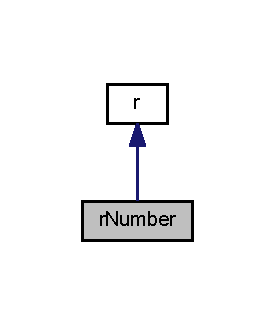
\includegraphics[width=132pt]{class_pierce_moore_1_1_ruby_p_h_p_1_1r_number__inherit__graph}
\end{center}
\end{figure}


Collaboration diagram for r\-Number\-:
\nopagebreak
\begin{figure}[H]
\begin{center}
\leavevmode
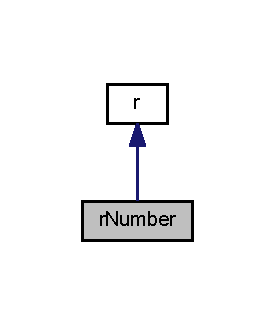
\includegraphics[width=132pt]{class_pierce_moore_1_1_ruby_p_h_p_1_1r_number__coll__graph}
\end{center}
\end{figure}
\subsection*{Public Member Functions}
\begin{DoxyCompactItemize}
\item 
\hyperlink{class_pierce_moore_1_1_ruby_p_h_p_1_1r_number_a4b0c1fe0e6c94ec2df5006f414b164c4}{\-\_\-\-\_\-construct} (\$item)
\item 
\hyperlink{class_pierce_moore_1_1_ruby_p_h_p_1_1r_number_a686a6d6caa2f0a26bede859f3d180c83}{build\-Number} ()
\item 
\hyperlink{class_pierce_moore_1_1_ruby_p_h_p_1_1r_number_a7755db2baa1c58774d9cf1c5c82676a1}{money} (\$symbol=\char`\"{}\$\char`\"{}, \$decimal=\char`\"{}.\char`\"{})
\item 
\hyperlink{class_pierce_moore_1_1_ruby_p_h_p_1_1r_number_a046b5f5e8b171d4724f2780303239825}{even} ()
\item 
\hyperlink{class_pierce_moore_1_1_ruby_p_h_p_1_1r_number_a666c4ea82d473f0e68ad97e3f33d1e83}{odd} ()
\item 
\hyperlink{class_pierce_moore_1_1_ruby_p_h_p_1_1r_number_a57202f5e3d5e0a89e18aac7d96773cab}{mult} (\$times)
\item 
\hyperlink{class_pierce_moore_1_1_ruby_p_h_p_1_1r_number_ad8c557c876471daa5dce718f01fd77b2}{av} ()
\item 
\hyperlink{class_pierce_moore_1_1_ruby_p_h_p_1_1r_number_a0a13d13bfe0866bab479a700d059898b}{gcd} (\$comparison)
\item 
\hyperlink{class_pierce_moore_1_1_ruby_p_h_p_1_1r_number_ab7cf083b6111db8f56b7d0b42cbba7a0}{rnd} (\$place)
\item 
\hyperlink{class_pierce_moore_1_1_ruby_p_h_p_1_1r_number_a63f86e65e715320e6e292251810cd0b9}{infinite} ()
\item 
\hyperlink{class_pierce_moore_1_1_ruby_p_h_p_1_1r_number_ae27ea99fd73ded7a863a154be23756d3}{Na\-N} ()
\item 
\hyperlink{class_pierce_moore_1_1_ruby_p_h_p_1_1r_number_a75525252dfe9a4b2cc4e31bf066afe1c}{zero} ()
\item 
\hyperlink{class_pierce_moore_1_1_ruby_p_h_p_1_1r_number_a0c6f82bc490087648b9f1fef553e05eb}{hex} ()
\item 
\hyperlink{class_pierce_moore_1_1_ruby_p_h_p_1_1r_number_a59e26fcd3f578f30737550623859abe7}{to\-Hex} ()
\end{DoxyCompactItemize}


\subsection{Detailed Description}


Definition at line 13 of file class.\-number.\-rubyphp.\-php.



\subsection{Constructor \& Destructor Documentation}
\hypertarget{class_pierce_moore_1_1_ruby_p_h_p_1_1r_number_a4b0c1fe0e6c94ec2df5006f414b164c4}{\index{Pierce\-Moore\-::\-Ruby\-P\-H\-P\-::r\-Number@{Pierce\-Moore\-::\-Ruby\-P\-H\-P\-::r\-Number}!\-\_\-\-\_\-construct@{\-\_\-\-\_\-construct}}
\index{\-\_\-\-\_\-construct@{\-\_\-\-\_\-construct}!PierceMoore::RubyPHP::rNumber@{Pierce\-Moore\-::\-Ruby\-P\-H\-P\-::r\-Number}}
\subsubsection[{\-\_\-\-\_\-construct}]{\setlength{\rightskip}{0pt plus 5cm}{\bf \-\_\-\-\_\-construct} (
\begin{DoxyParamCaption}
\item[{\$}]{item}
\end{DoxyParamCaption}
)}}\label{class_pierce_moore_1_1_ruby_p_h_p_1_1r_number_a4b0c1fe0e6c94ec2df5006f414b164c4}


Definition at line 15 of file class.\-number.\-rubyphp.\-php.



Here is the call graph for this function\-:
\nopagebreak
\begin{figure}[H]
\begin{center}
\leavevmode
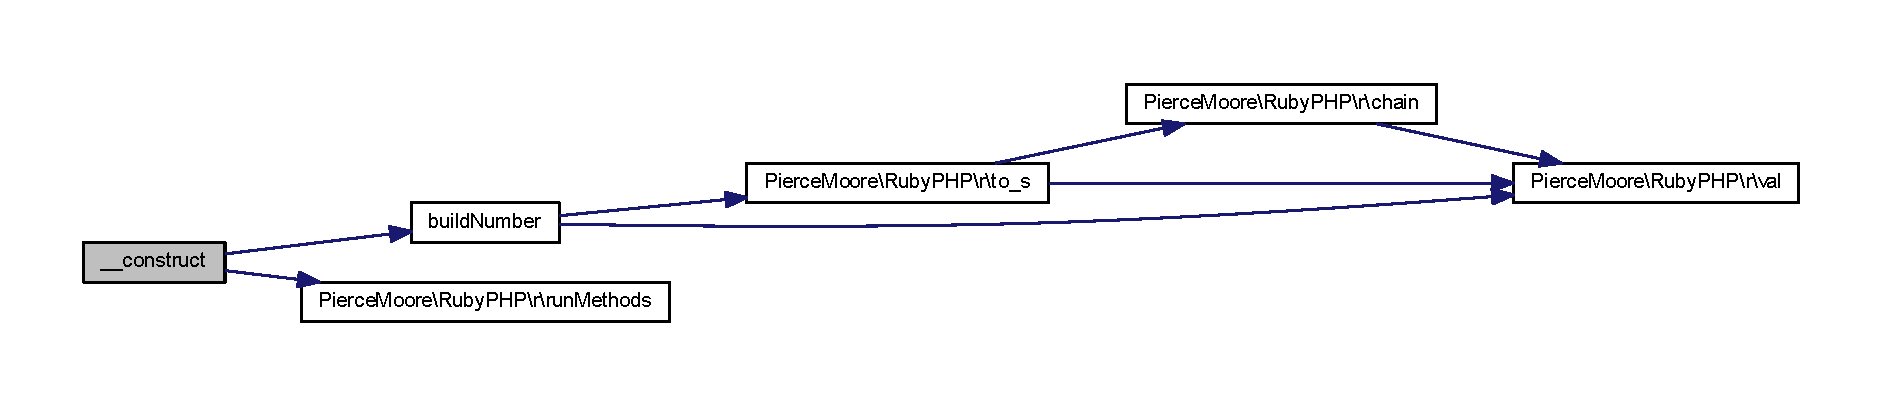
\includegraphics[width=350pt]{class_pierce_moore_1_1_ruby_p_h_p_1_1r_number_a4b0c1fe0e6c94ec2df5006f414b164c4_cgraph}
\end{center}
\end{figure}




\subsection{Member Function Documentation}
\hypertarget{class_pierce_moore_1_1_ruby_p_h_p_1_1r_number_ad8c557c876471daa5dce718f01fd77b2}{\index{Pierce\-Moore\-::\-Ruby\-P\-H\-P\-::r\-Number@{Pierce\-Moore\-::\-Ruby\-P\-H\-P\-::r\-Number}!av@{av}}
\index{av@{av}!PierceMoore::RubyPHP::rNumber@{Pierce\-Moore\-::\-Ruby\-P\-H\-P\-::r\-Number}}
\subsubsection[{av}]{\setlength{\rightskip}{0pt plus 5cm}{\bf av} (
\begin{DoxyParamCaption}
{}
\end{DoxyParamCaption}
)}}\label{class_pierce_moore_1_1_ruby_p_h_p_1_1r_number_ad8c557c876471daa5dce718f01fd77b2}
\begin{DoxyReturn}{Returns}
mixed 
\end{DoxyReturn}


Definition at line 136 of file class.\-number.\-rubyphp.\-php.



Here is the call graph for this function\-:
\nopagebreak
\begin{figure}[H]
\begin{center}
\leavevmode
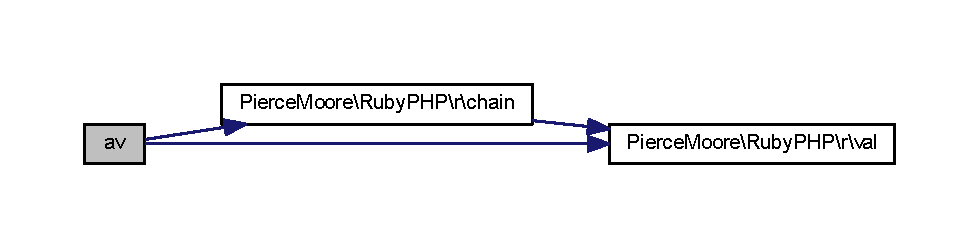
\includegraphics[width=350pt]{class_pierce_moore_1_1_ruby_p_h_p_1_1r_number_ad8c557c876471daa5dce718f01fd77b2_cgraph}
\end{center}
\end{figure}


\hypertarget{class_pierce_moore_1_1_ruby_p_h_p_1_1r_number_a686a6d6caa2f0a26bede859f3d180c83}{\index{Pierce\-Moore\-::\-Ruby\-P\-H\-P\-::r\-Number@{Pierce\-Moore\-::\-Ruby\-P\-H\-P\-::r\-Number}!build\-Number@{build\-Number}}
\index{build\-Number@{build\-Number}!PierceMoore::RubyPHP::rNumber@{Pierce\-Moore\-::\-Ruby\-P\-H\-P\-::r\-Number}}
\subsubsection[{build\-Number}]{\setlength{\rightskip}{0pt plus 5cm}{\bf build\-Number} (
\begin{DoxyParamCaption}
{}
\end{DoxyParamCaption}
)}}\label{class_pierce_moore_1_1_ruby_p_h_p_1_1r_number_a686a6d6caa2f0a26bede859f3d180c83}


Definition at line 29 of file class.\-number.\-rubyphp.\-php.



Here is the call graph for this function\-:
\nopagebreak
\begin{figure}[H]
\begin{center}
\leavevmode
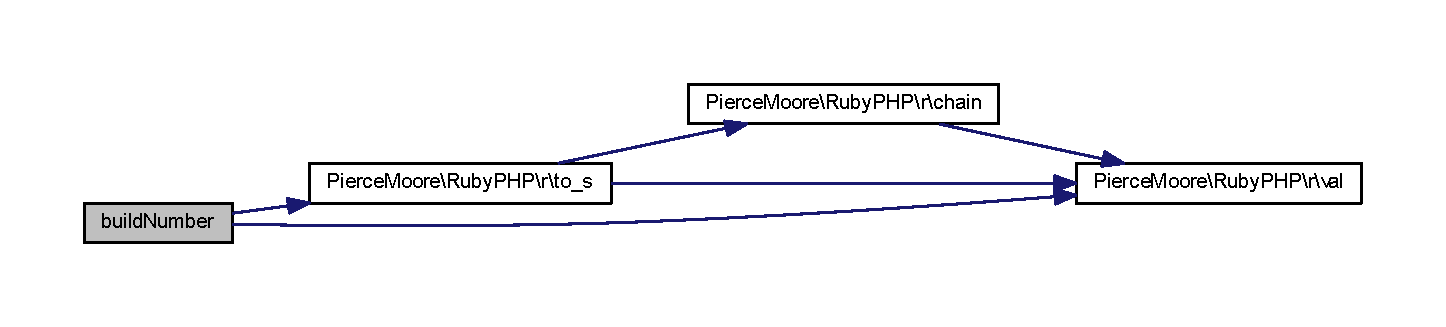
\includegraphics[width=350pt]{class_pierce_moore_1_1_ruby_p_h_p_1_1r_number_a686a6d6caa2f0a26bede859f3d180c83_cgraph}
\end{center}
\end{figure}




Here is the caller graph for this function\-:
\nopagebreak
\begin{figure}[H]
\begin{center}
\leavevmode
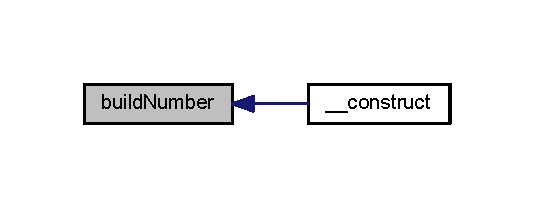
\includegraphics[width=256pt]{class_pierce_moore_1_1_ruby_p_h_p_1_1r_number_a686a6d6caa2f0a26bede859f3d180c83_icgraph}
\end{center}
\end{figure}


\hypertarget{class_pierce_moore_1_1_ruby_p_h_p_1_1r_number_a046b5f5e8b171d4724f2780303239825}{\index{Pierce\-Moore\-::\-Ruby\-P\-H\-P\-::r\-Number@{Pierce\-Moore\-::\-Ruby\-P\-H\-P\-::r\-Number}!even@{even}}
\index{even@{even}!PierceMoore::RubyPHP::rNumber@{Pierce\-Moore\-::\-Ruby\-P\-H\-P\-::r\-Number}}
\subsubsection[{even}]{\setlength{\rightskip}{0pt plus 5cm}{\bf even} (
\begin{DoxyParamCaption}
{}
\end{DoxyParamCaption}
)}}\label{class_pierce_moore_1_1_ruby_p_h_p_1_1r_number_a046b5f5e8b171d4724f2780303239825}
\begin{DoxyReturn}{Returns}
boolean 
\end{DoxyReturn}


Definition at line 75 of file class.\-number.\-rubyphp.\-php.



Here is the call graph for this function\-:
\nopagebreak
\begin{figure}[H]
\begin{center}
\leavevmode
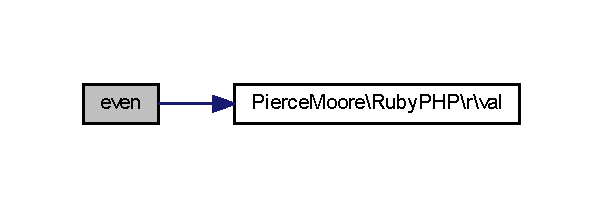
\includegraphics[width=290pt]{class_pierce_moore_1_1_ruby_p_h_p_1_1r_number_a046b5f5e8b171d4724f2780303239825_cgraph}
\end{center}
\end{figure}


\hypertarget{class_pierce_moore_1_1_ruby_p_h_p_1_1r_number_a0a13d13bfe0866bab479a700d059898b}{\index{Pierce\-Moore\-::\-Ruby\-P\-H\-P\-::r\-Number@{Pierce\-Moore\-::\-Ruby\-P\-H\-P\-::r\-Number}!gcd@{gcd}}
\index{gcd@{gcd}!PierceMoore::RubyPHP::rNumber@{Pierce\-Moore\-::\-Ruby\-P\-H\-P\-::r\-Number}}
\subsubsection[{gcd}]{\setlength{\rightskip}{0pt plus 5cm}{\bf gcd} (
\begin{DoxyParamCaption}
\item[{\$}]{comparison}
\end{DoxyParamCaption}
)}}\label{class_pierce_moore_1_1_ruby_p_h_p_1_1r_number_a0a13d13bfe0866bab479a700d059898b}

\begin{DoxyParams}[1]{Parameters}
mixed & {\em \$comparison} & -\/ The number to find the G\-C\-D with \\
\hline
\end{DoxyParams}
\begin{DoxyReturn}{Returns}
mixed 
\end{DoxyReturn}


Definition at line 151 of file class.\-number.\-rubyphp.\-php.



Here is the call graph for this function\-:
\nopagebreak
\begin{figure}[H]
\begin{center}
\leavevmode
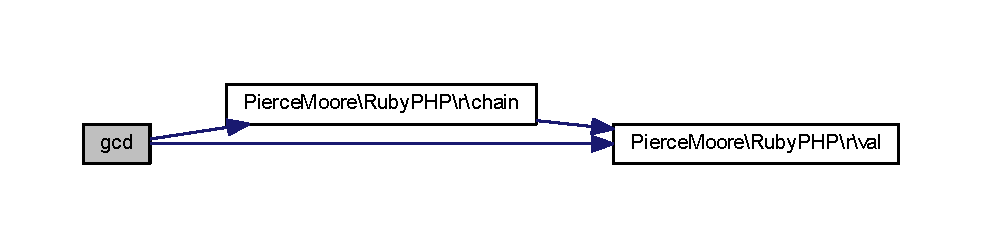
\includegraphics[width=350pt]{class_pierce_moore_1_1_ruby_p_h_p_1_1r_number_a0a13d13bfe0866bab479a700d059898b_cgraph}
\end{center}
\end{figure}


\hypertarget{class_pierce_moore_1_1_ruby_p_h_p_1_1r_number_a0c6f82bc490087648b9f1fef553e05eb}{\index{Pierce\-Moore\-::\-Ruby\-P\-H\-P\-::r\-Number@{Pierce\-Moore\-::\-Ruby\-P\-H\-P\-::r\-Number}!hex@{hex}}
\index{hex@{hex}!PierceMoore::RubyPHP::rNumber@{Pierce\-Moore\-::\-Ruby\-P\-H\-P\-::r\-Number}}
\subsubsection[{hex}]{\setlength{\rightskip}{0pt plus 5cm}{\bf hex} (
\begin{DoxyParamCaption}
{}
\end{DoxyParamCaption}
)}}\label{class_pierce_moore_1_1_ruby_p_h_p_1_1r_number_a0c6f82bc490087648b9f1fef553e05eb}
\begin{DoxyReturn}{Returns}
mixed 
\end{DoxyReturn}


Definition at line 239 of file class.\-number.\-rubyphp.\-php.



Here is the call graph for this function\-:
\nopagebreak
\begin{figure}[H]
\begin{center}
\leavevmode
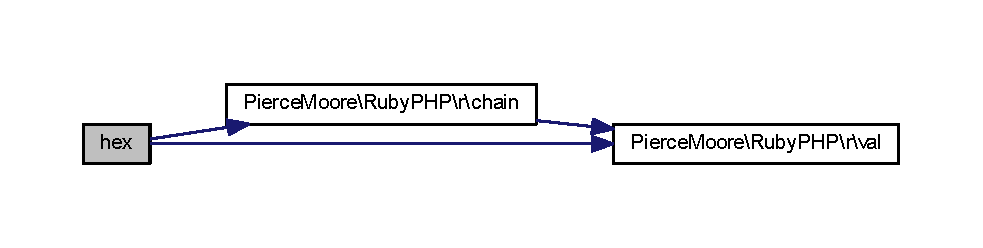
\includegraphics[width=350pt]{class_pierce_moore_1_1_ruby_p_h_p_1_1r_number_a0c6f82bc490087648b9f1fef553e05eb_cgraph}
\end{center}
\end{figure}


\hypertarget{class_pierce_moore_1_1_ruby_p_h_p_1_1r_number_a63f86e65e715320e6e292251810cd0b9}{\index{Pierce\-Moore\-::\-Ruby\-P\-H\-P\-::r\-Number@{Pierce\-Moore\-::\-Ruby\-P\-H\-P\-::r\-Number}!infinite@{infinite}}
\index{infinite@{infinite}!PierceMoore::RubyPHP::rNumber@{Pierce\-Moore\-::\-Ruby\-P\-H\-P\-::r\-Number}}
\subsubsection[{infinite}]{\setlength{\rightskip}{0pt plus 5cm}{\bf infinite} (
\begin{DoxyParamCaption}
{}
\end{DoxyParamCaption}
)}}\label{class_pierce_moore_1_1_ruby_p_h_p_1_1r_number_a63f86e65e715320e6e292251810cd0b9}
\begin{DoxyReturn}{Returns}
boolean 
\end{DoxyReturn}


Definition at line 183 of file class.\-number.\-rubyphp.\-php.



Here is the call graph for this function\-:
\nopagebreak
\begin{figure}[H]
\begin{center}
\leavevmode
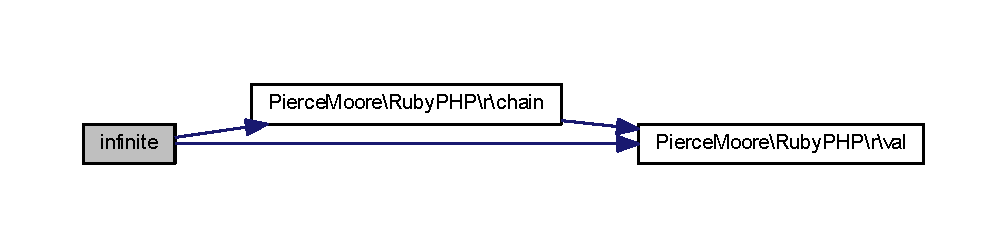
\includegraphics[width=350pt]{class_pierce_moore_1_1_ruby_p_h_p_1_1r_number_a63f86e65e715320e6e292251810cd0b9_cgraph}
\end{center}
\end{figure}


\hypertarget{class_pierce_moore_1_1_ruby_p_h_p_1_1r_number_a7755db2baa1c58774d9cf1c5c82676a1}{\index{Pierce\-Moore\-::\-Ruby\-P\-H\-P\-::r\-Number@{Pierce\-Moore\-::\-Ruby\-P\-H\-P\-::r\-Number}!money@{money}}
\index{money@{money}!PierceMoore::RubyPHP::rNumber@{Pierce\-Moore\-::\-Ruby\-P\-H\-P\-::r\-Number}}
\subsubsection[{money}]{\setlength{\rightskip}{0pt plus 5cm}{\bf money} (
\begin{DoxyParamCaption}
\item[{\$}]{symbol = {\ttfamily \char`\"{}\$\char`\"{}}, }
\item[{\$}]{decimal = {\ttfamily \char`\"{}.\char`\"{}}}
\end{DoxyParamCaption}
)}}\label{class_pierce_moore_1_1_ruby_p_h_p_1_1r_number_a7755db2baa1c58774d9cf1c5c82676a1}

\begin{DoxyParams}[1]{Parameters}
string & {\em \$symbol} & -\/ The currency denominator to use \\
\hline
string & {\em \$decimal} & -\/ The decimal separator \\
\hline
\end{DoxyParams}
\begin{DoxyReturn}{Returns}
string 
\end{DoxyReturn}


Definition at line 52 of file class.\-number.\-rubyphp.\-php.



Here is the call graph for this function\-:
\nopagebreak
\begin{figure}[H]
\begin{center}
\leavevmode
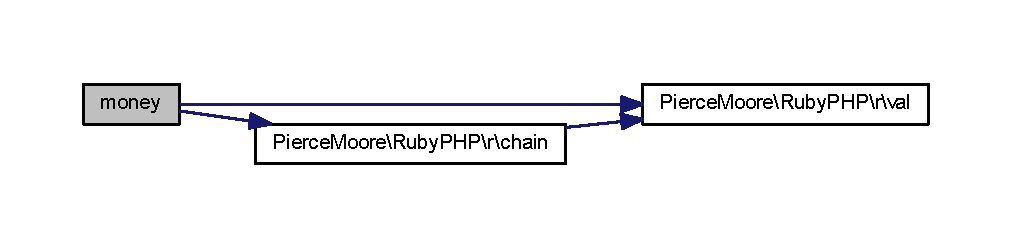
\includegraphics[width=350pt]{class_pierce_moore_1_1_ruby_p_h_p_1_1r_number_a7755db2baa1c58774d9cf1c5c82676a1_cgraph}
\end{center}
\end{figure}


\hypertarget{class_pierce_moore_1_1_ruby_p_h_p_1_1r_number_a57202f5e3d5e0a89e18aac7d96773cab}{\index{Pierce\-Moore\-::\-Ruby\-P\-H\-P\-::r\-Number@{Pierce\-Moore\-::\-Ruby\-P\-H\-P\-::r\-Number}!mult@{mult}}
\index{mult@{mult}!PierceMoore::RubyPHP::rNumber@{Pierce\-Moore\-::\-Ruby\-P\-H\-P\-::r\-Number}}
\subsubsection[{mult}]{\setlength{\rightskip}{0pt plus 5cm}{\bf mult} (
\begin{DoxyParamCaption}
\item[{\$}]{times}
\end{DoxyParamCaption}
)}}\label{class_pierce_moore_1_1_ruby_p_h_p_1_1r_number_a57202f5e3d5e0a89e18aac7d96773cab}

\begin{DoxyParams}[1]{Parameters}
mixed & {\em \$times} & -\/ The multiplier \\
\hline
\end{DoxyParams}
\begin{DoxyReturn}{Returns}
mixed 
\end{DoxyReturn}


Definition at line 122 of file class.\-number.\-rubyphp.\-php.



Here is the call graph for this function\-:
\nopagebreak
\begin{figure}[H]
\begin{center}
\leavevmode
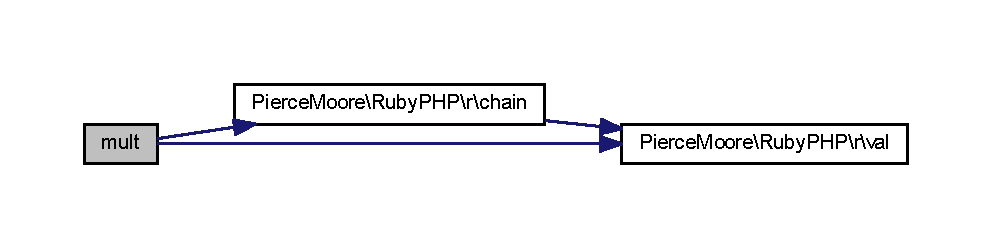
\includegraphics[width=350pt]{class_pierce_moore_1_1_ruby_p_h_p_1_1r_number_a57202f5e3d5e0a89e18aac7d96773cab_cgraph}
\end{center}
\end{figure}


\hypertarget{class_pierce_moore_1_1_ruby_p_h_p_1_1r_number_ae27ea99fd73ded7a863a154be23756d3}{\index{Pierce\-Moore\-::\-Ruby\-P\-H\-P\-::r\-Number@{Pierce\-Moore\-::\-Ruby\-P\-H\-P\-::r\-Number}!Na\-N@{Na\-N}}
\index{Na\-N@{Na\-N}!PierceMoore::RubyPHP::rNumber@{Pierce\-Moore\-::\-Ruby\-P\-H\-P\-::r\-Number}}
\subsubsection[{Na\-N}]{\setlength{\rightskip}{0pt plus 5cm}{\bf Na\-N} (
\begin{DoxyParamCaption}
{}
\end{DoxyParamCaption}
)}}\label{class_pierce_moore_1_1_ruby_p_h_p_1_1r_number_ae27ea99fd73ded7a863a154be23756d3}
\begin{DoxyReturn}{Returns}
boolean 
\end{DoxyReturn}


Definition at line 197 of file class.\-number.\-rubyphp.\-php.



Here is the call graph for this function\-:
\nopagebreak
\begin{figure}[H]
\begin{center}
\leavevmode
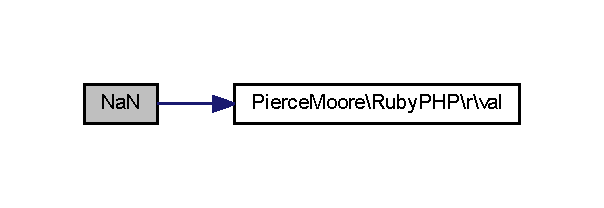
\includegraphics[width=290pt]{class_pierce_moore_1_1_ruby_p_h_p_1_1r_number_ae27ea99fd73ded7a863a154be23756d3_cgraph}
\end{center}
\end{figure}




Here is the caller graph for this function\-:
\nopagebreak
\begin{figure}[H]
\begin{center}
\leavevmode
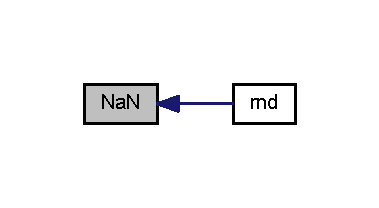
\includegraphics[width=182pt]{class_pierce_moore_1_1_ruby_p_h_p_1_1r_number_ae27ea99fd73ded7a863a154be23756d3_icgraph}
\end{center}
\end{figure}


\hypertarget{class_pierce_moore_1_1_ruby_p_h_p_1_1r_number_a666c4ea82d473f0e68ad97e3f33d1e83}{\index{Pierce\-Moore\-::\-Ruby\-P\-H\-P\-::r\-Number@{Pierce\-Moore\-::\-Ruby\-P\-H\-P\-::r\-Number}!odd@{odd}}
\index{odd@{odd}!PierceMoore::RubyPHP::rNumber@{Pierce\-Moore\-::\-Ruby\-P\-H\-P\-::r\-Number}}
\subsubsection[{odd}]{\setlength{\rightskip}{0pt plus 5cm}{\bf odd} (
\begin{DoxyParamCaption}
{}
\end{DoxyParamCaption}
)}}\label{class_pierce_moore_1_1_ruby_p_h_p_1_1r_number_a666c4ea82d473f0e68ad97e3f33d1e83}
\begin{DoxyReturn}{Returns}
boolean 
\end{DoxyReturn}


Definition at line 98 of file class.\-number.\-rubyphp.\-php.



Here is the call graph for this function\-:
\nopagebreak
\begin{figure}[H]
\begin{center}
\leavevmode
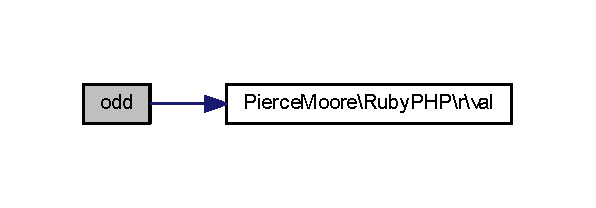
\includegraphics[width=286pt]{class_pierce_moore_1_1_ruby_p_h_p_1_1r_number_a666c4ea82d473f0e68ad97e3f33d1e83_cgraph}
\end{center}
\end{figure}


\hypertarget{class_pierce_moore_1_1_ruby_p_h_p_1_1r_number_ab7cf083b6111db8f56b7d0b42cbba7a0}{\index{Pierce\-Moore\-::\-Ruby\-P\-H\-P\-::r\-Number@{Pierce\-Moore\-::\-Ruby\-P\-H\-P\-::r\-Number}!rnd@{rnd}}
\index{rnd@{rnd}!PierceMoore::RubyPHP::rNumber@{Pierce\-Moore\-::\-Ruby\-P\-H\-P\-::r\-Number}}
\subsubsection[{rnd}]{\setlength{\rightskip}{0pt plus 5cm}{\bf rnd} (
\begin{DoxyParamCaption}
\item[{\$}]{place}
\end{DoxyParamCaption}
)}}\label{class_pierce_moore_1_1_ruby_p_h_p_1_1r_number_ab7cf083b6111db8f56b7d0b42cbba7a0}

\begin{DoxyParams}[1]{Parameters}
int & {\em \$place} & -\/ The precision with which you would like to round the number. \\
\hline
\end{DoxyParams}
\begin{DoxyReturn}{Returns}
mixed 
\end{DoxyReturn}


Definition at line 166 of file class.\-number.\-rubyphp.\-php.



Here is the call graph for this function\-:
\nopagebreak
\begin{figure}[H]
\begin{center}
\leavevmode
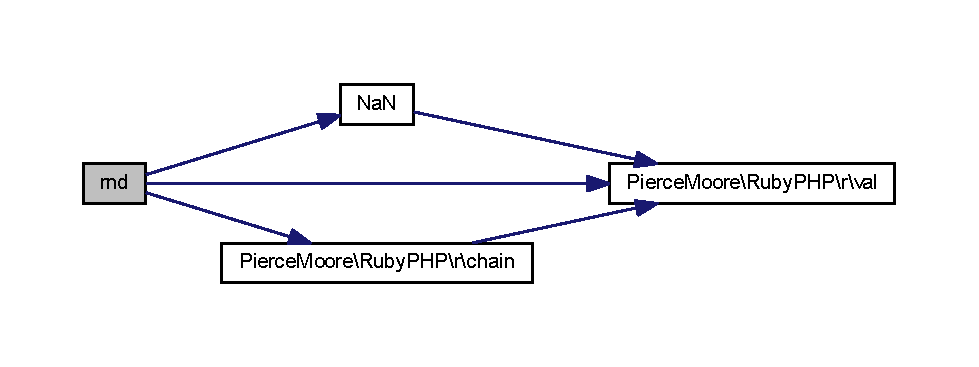
\includegraphics[width=350pt]{class_pierce_moore_1_1_ruby_p_h_p_1_1r_number_ab7cf083b6111db8f56b7d0b42cbba7a0_cgraph}
\end{center}
\end{figure}


\hypertarget{class_pierce_moore_1_1_ruby_p_h_p_1_1r_number_a59e26fcd3f578f30737550623859abe7}{\index{Pierce\-Moore\-::\-Ruby\-P\-H\-P\-::r\-Number@{Pierce\-Moore\-::\-Ruby\-P\-H\-P\-::r\-Number}!to\-Hex@{to\-Hex}}
\index{to\-Hex@{to\-Hex}!PierceMoore::RubyPHP::rNumber@{Pierce\-Moore\-::\-Ruby\-P\-H\-P\-::r\-Number}}
\subsubsection[{to\-Hex}]{\setlength{\rightskip}{0pt plus 5cm}{\bf to\-Hex} (
\begin{DoxyParamCaption}
{}
\end{DoxyParamCaption}
)}}\label{class_pierce_moore_1_1_ruby_p_h_p_1_1r_number_a59e26fcd3f578f30737550623859abe7}
\begin{DoxyReturn}{Returns}
mixed 
\end{DoxyReturn}


Definition at line 257 of file class.\-number.\-rubyphp.\-php.



Here is the call graph for this function\-:
\nopagebreak
\begin{figure}[H]
\begin{center}
\leavevmode
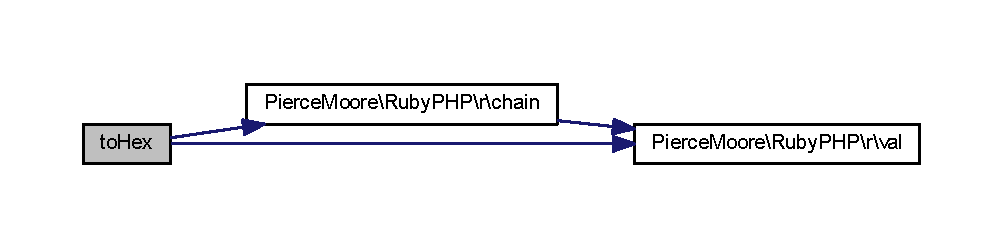
\includegraphics[width=350pt]{class_pierce_moore_1_1_ruby_p_h_p_1_1r_number_a59e26fcd3f578f30737550623859abe7_cgraph}
\end{center}
\end{figure}


\hypertarget{class_pierce_moore_1_1_ruby_p_h_p_1_1r_number_a75525252dfe9a4b2cc4e31bf066afe1c}{\index{Pierce\-Moore\-::\-Ruby\-P\-H\-P\-::r\-Number@{Pierce\-Moore\-::\-Ruby\-P\-H\-P\-::r\-Number}!zero@{zero}}
\index{zero@{zero}!PierceMoore::RubyPHP::rNumber@{Pierce\-Moore\-::\-Ruby\-P\-H\-P\-::r\-Number}}
\subsubsection[{zero}]{\setlength{\rightskip}{0pt plus 5cm}{\bf zero} (
\begin{DoxyParamCaption}
{}
\end{DoxyParamCaption}
)}}\label{class_pierce_moore_1_1_ruby_p_h_p_1_1r_number_a75525252dfe9a4b2cc4e31bf066afe1c}
\begin{DoxyReturn}{Returns}
boolean 
\end{DoxyReturn}


Definition at line 216 of file class.\-number.\-rubyphp.\-php.



Here is the call graph for this function\-:
\nopagebreak
\begin{figure}[H]
\begin{center}
\leavevmode
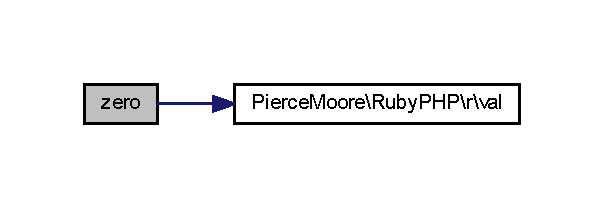
\includegraphics[width=290pt]{class_pierce_moore_1_1_ruby_p_h_p_1_1r_number_a75525252dfe9a4b2cc4e31bf066afe1c_cgraph}
\end{center}
\end{figure}




The documentation for this class was generated from the following file\-:\begin{DoxyCompactItemize}
\item 
Ruby\-P\-H\-P/includes/\hyperlink{class_8number_8rubyphp_8php}{class.\-number.\-rubyphp.\-php}\end{DoxyCompactItemize}

\hypertarget{class_pierce_moore_1_1_ruby_p_h_p_1_1r_string}{\section{r\-String Class Reference}
\label{class_pierce_moore_1_1_ruby_p_h_p_1_1r_string}\index{r\-String@{r\-String}}
}


Inheritance diagram for r\-String\-:
\nopagebreak
\begin{figure}[H]
\begin{center}
\leavevmode
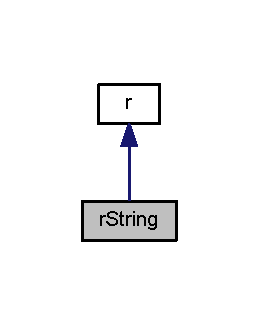
\includegraphics[width=124pt]{class_pierce_moore_1_1_ruby_p_h_p_1_1r_string__inherit__graph}
\end{center}
\end{figure}


Collaboration diagram for r\-String\-:
\nopagebreak
\begin{figure}[H]
\begin{center}
\leavevmode
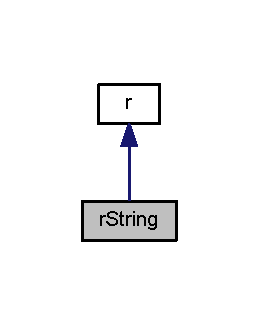
\includegraphics[width=124pt]{class_pierce_moore_1_1_ruby_p_h_p_1_1r_string__coll__graph}
\end{center}
\end{figure}
\subsection*{Public Member Functions}
\begin{DoxyCompactItemize}
\item 
\hyperlink{class_pierce_moore_1_1_ruby_p_h_p_1_1r_string_a4b0c1fe0e6c94ec2df5006f414b164c4}{\-\_\-\-\_\-construct} (\$item)
\item 
\hyperlink{class_pierce_moore_1_1_ruby_p_h_p_1_1r_string_a52486765aad19321ca30127f786ca709}{each\-\_\-char} (\$function)
\item 
\hyperlink{class_pierce_moore_1_1_ruby_p_h_p_1_1r_string_a93130ece3f9aced2dcacf00ec6968413}{tr} ()
\item 
\hyperlink{class_pierce_moore_1_1_ruby_p_h_p_1_1r_string_ab4e6060d5b0dd93113194ba83534d385}{escape} ()
\item 
\hyperlink{class_pierce_moore_1_1_ruby_p_h_p_1_1r_string_a6919ea74ebb93cd28fee10d172ebc4c4}{cap} (\$type, \$value=null)
\item 
\hyperlink{class_pierce_moore_1_1_ruby_p_h_p_1_1r_string_a04980c8e9024c09c700fdf68df9d5775}{swapcase} ()
\end{DoxyCompactItemize}
\subsection*{Protected Member Functions}
\begin{DoxyCompactItemize}
\item 
\hyperlink{class_pierce_moore_1_1_ruby_p_h_p_1_1r_string_a6162696233b36efd30e0617c0e51a691}{build\-String} ()
\end{DoxyCompactItemize}


\subsection{Detailed Description}


Definition at line 13 of file class.\-string.\-rubyphp.\-php.



\subsection{Constructor \& Destructor Documentation}
\hypertarget{class_pierce_moore_1_1_ruby_p_h_p_1_1r_string_a4b0c1fe0e6c94ec2df5006f414b164c4}{\index{Pierce\-Moore\-::\-Ruby\-P\-H\-P\-::r\-String@{Pierce\-Moore\-::\-Ruby\-P\-H\-P\-::r\-String}!\-\_\-\-\_\-construct@{\-\_\-\-\_\-construct}}
\index{\-\_\-\-\_\-construct@{\-\_\-\-\_\-construct}!PierceMoore::RubyPHP::rString@{Pierce\-Moore\-::\-Ruby\-P\-H\-P\-::r\-String}}
\subsubsection[{\-\_\-\-\_\-construct}]{\setlength{\rightskip}{0pt plus 5cm}{\bf \-\_\-\-\_\-construct} (
\begin{DoxyParamCaption}
\item[{\$}]{item}
\end{DoxyParamCaption}
)}}\label{class_pierce_moore_1_1_ruby_p_h_p_1_1r_string_a4b0c1fe0e6c94ec2df5006f414b164c4}


Definition at line 15 of file class.\-string.\-rubyphp.\-php.



Here is the call graph for this function\-:
\nopagebreak
\begin{figure}[H]
\begin{center}
\leavevmode
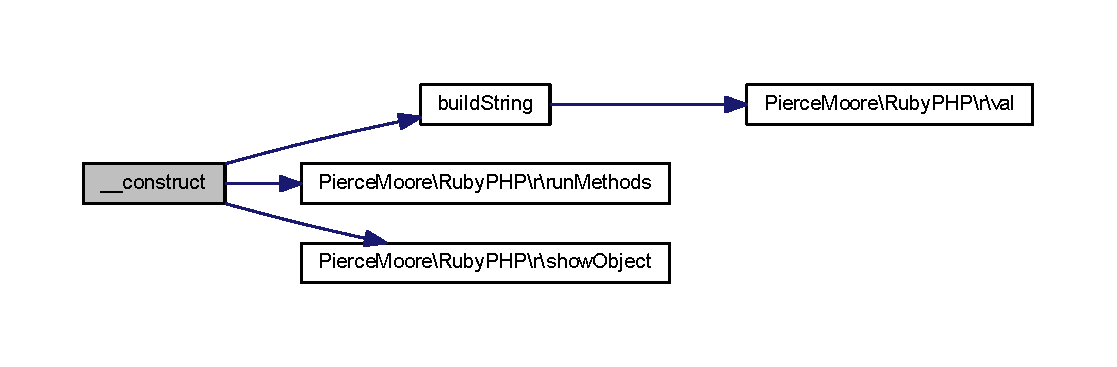
\includegraphics[width=350pt]{class_pierce_moore_1_1_ruby_p_h_p_1_1r_string_a4b0c1fe0e6c94ec2df5006f414b164c4_cgraph}
\end{center}
\end{figure}




\subsection{Member Function Documentation}
\hypertarget{class_pierce_moore_1_1_ruby_p_h_p_1_1r_string_a6162696233b36efd30e0617c0e51a691}{\index{Pierce\-Moore\-::\-Ruby\-P\-H\-P\-::r\-String@{Pierce\-Moore\-::\-Ruby\-P\-H\-P\-::r\-String}!build\-String@{build\-String}}
\index{build\-String@{build\-String}!PierceMoore::RubyPHP::rString@{Pierce\-Moore\-::\-Ruby\-P\-H\-P\-::r\-String}}
\subsubsection[{build\-String}]{\setlength{\rightskip}{0pt plus 5cm}{\bf build\-String} (
\begin{DoxyParamCaption}
{}
\end{DoxyParamCaption}
)\hspace{0.3cm}{\ttfamily  \mbox{[}protected\mbox{]}}}}\label{class_pierce_moore_1_1_ruby_p_h_p_1_1r_string_a6162696233b36efd30e0617c0e51a691}
\begin{DoxyReturn}{Returns}
boolean 
\end{DoxyReturn}


Definition at line 30 of file class.\-string.\-rubyphp.\-php.



Here is the call graph for this function\-:
\nopagebreak
\begin{figure}[H]
\begin{center}
\leavevmode
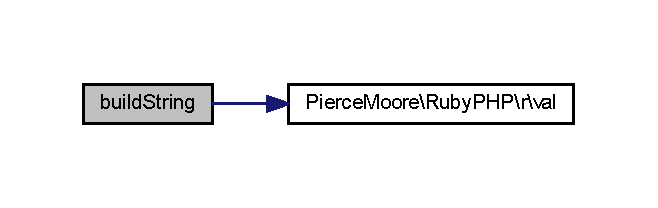
\includegraphics[width=316pt]{class_pierce_moore_1_1_ruby_p_h_p_1_1r_string_a6162696233b36efd30e0617c0e51a691_cgraph}
\end{center}
\end{figure}




Here is the caller graph for this function\-:
\nopagebreak
\begin{figure}[H]
\begin{center}
\leavevmode
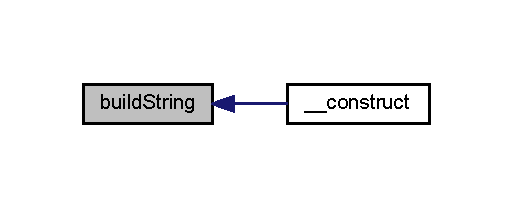
\includegraphics[width=246pt]{class_pierce_moore_1_1_ruby_p_h_p_1_1r_string_a6162696233b36efd30e0617c0e51a691_icgraph}
\end{center}
\end{figure}


\hypertarget{class_pierce_moore_1_1_ruby_p_h_p_1_1r_string_a6919ea74ebb93cd28fee10d172ebc4c4}{\index{Pierce\-Moore\-::\-Ruby\-P\-H\-P\-::r\-String@{Pierce\-Moore\-::\-Ruby\-P\-H\-P\-::r\-String}!cap@{cap}}
\index{cap@{cap}!PierceMoore::RubyPHP::rString@{Pierce\-Moore\-::\-Ruby\-P\-H\-P\-::r\-String}}
\subsubsection[{cap}]{\setlength{\rightskip}{0pt plus 5cm}{\bf cap} (
\begin{DoxyParamCaption}
\item[{\$}]{type, }
\item[{\$}]{value = {\ttfamily null}}
\end{DoxyParamCaption}
)}}\label{class_pierce_moore_1_1_ruby_p_h_p_1_1r_string_a6919ea74ebb93cd28fee10d172ebc4c4}

\begin{DoxyParams}[1]{Parameters}
string & {\em \$type} & -\/ The parameters that the capitalize function must work within. Accepts\-: \char`\"{}first\char`\"{} , \char`\"{}all\char`\"{} , \char`\"{}none\char`\"{} , \char`\"{}words\char`\"{} \\
\hline
mixed & {\em \$value} & -\/ The value to be modified. I found that this parameter was necessary for other functions that required casing and needed to pass their own values. \\
\hline
\end{DoxyParams}
\begin{DoxyReturn}{Returns}
string 
\end{DoxyReturn}


Definition at line 104 of file class.\-string.\-rubyphp.\-php.



Here is the call graph for this function\-:
\nopagebreak
\begin{figure}[H]
\begin{center}
\leavevmode
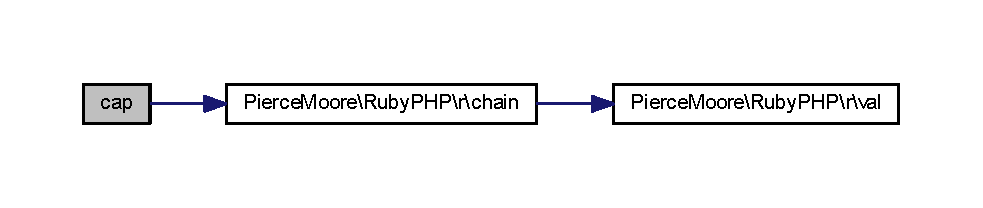
\includegraphics[width=350pt]{class_pierce_moore_1_1_ruby_p_h_p_1_1r_string_a6919ea74ebb93cd28fee10d172ebc4c4_cgraph}
\end{center}
\end{figure}


\hypertarget{class_pierce_moore_1_1_ruby_p_h_p_1_1r_string_a52486765aad19321ca30127f786ca709}{\index{Pierce\-Moore\-::\-Ruby\-P\-H\-P\-::r\-String@{Pierce\-Moore\-::\-Ruby\-P\-H\-P\-::r\-String}!each\-\_\-char@{each\-\_\-char}}
\index{each\-\_\-char@{each\-\_\-char}!PierceMoore::RubyPHP::rString@{Pierce\-Moore\-::\-Ruby\-P\-H\-P\-::r\-String}}
\subsubsection[{each\-\_\-char}]{\setlength{\rightskip}{0pt plus 5cm}{\bf each\-\_\-char} (
\begin{DoxyParamCaption}
\item[{\$}]{function}
\end{DoxyParamCaption}
)}}\label{class_pierce_moore_1_1_ruby_p_h_p_1_1r_string_a52486765aad19321ca30127f786ca709}

\begin{DoxyParams}[1]{Parameters}
string & {\em \$function} & -\/ The user-\/supplied function that will be run against the characters \\
\hline
\end{DoxyParams}
\begin{DoxyReturn}{Returns}
mixed 
\end{DoxyReturn}


Definition at line 47 of file class.\-string.\-rubyphp.\-php.



Here is the call graph for this function\-:
\nopagebreak
\begin{figure}[H]
\begin{center}
\leavevmode
\includegraphics[width=350pt]{class_pierce_moore_1_1_ruby_p_h_p_1_1r_string_a52486765aad19321ca30127f786ca709_cgraph}
\end{center}
\end{figure}


\hypertarget{class_pierce_moore_1_1_ruby_p_h_p_1_1r_string_ab4e6060d5b0dd93113194ba83534d385}{\index{Pierce\-Moore\-::\-Ruby\-P\-H\-P\-::r\-String@{Pierce\-Moore\-::\-Ruby\-P\-H\-P\-::r\-String}!escape@{escape}}
\index{escape@{escape}!PierceMoore::RubyPHP::rString@{Pierce\-Moore\-::\-Ruby\-P\-H\-P\-::r\-String}}
\subsubsection[{escape}]{\setlength{\rightskip}{0pt plus 5cm}{\bf escape} (
\begin{DoxyParamCaption}
{}
\end{DoxyParamCaption}
)}}\label{class_pierce_moore_1_1_ruby_p_h_p_1_1r_string_ab4e6060d5b0dd93113194ba83534d385}
\begin{DoxyReturn}{Returns}
string 
\end{DoxyReturn}


Definition at line 85 of file class.\-string.\-rubyphp.\-php.



Here is the call graph for this function\-:
\nopagebreak
\begin{figure}[H]
\begin{center}
\leavevmode
\includegraphics[width=350pt]{class_pierce_moore_1_1_ruby_p_h_p_1_1r_string_ab4e6060d5b0dd93113194ba83534d385_cgraph}
\end{center}
\end{figure}


\hypertarget{class_pierce_moore_1_1_ruby_p_h_p_1_1r_string_a04980c8e9024c09c700fdf68df9d5775}{\index{Pierce\-Moore\-::\-Ruby\-P\-H\-P\-::r\-String@{Pierce\-Moore\-::\-Ruby\-P\-H\-P\-::r\-String}!swapcase@{swapcase}}
\index{swapcase@{swapcase}!PierceMoore::RubyPHP::rString@{Pierce\-Moore\-::\-Ruby\-P\-H\-P\-::r\-String}}
\subsubsection[{swapcase}]{\setlength{\rightskip}{0pt plus 5cm}{\bf swapcase} (
\begin{DoxyParamCaption}
{}
\end{DoxyParamCaption}
)}}\label{class_pierce_moore_1_1_ruby_p_h_p_1_1r_string_a04980c8e9024c09c700fdf68df9d5775}
\begin{DoxyReturn}{Returns}
mixed 
\end{DoxyReturn}


Definition at line 139 of file class.\-string.\-rubyphp.\-php.



Here is the call graph for this function\-:
\nopagebreak
\begin{figure}[H]
\begin{center}
\leavevmode
\includegraphics[width=350pt]{class_pierce_moore_1_1_ruby_p_h_p_1_1r_string_a04980c8e9024c09c700fdf68df9d5775_cgraph}
\end{center}
\end{figure}


\hypertarget{class_pierce_moore_1_1_ruby_p_h_p_1_1r_string_a93130ece3f9aced2dcacf00ec6968413}{\index{Pierce\-Moore\-::\-Ruby\-P\-H\-P\-::r\-String@{Pierce\-Moore\-::\-Ruby\-P\-H\-P\-::r\-String}!tr@{tr}}
\index{tr@{tr}!PierceMoore::RubyPHP::rString@{Pierce\-Moore\-::\-Ruby\-P\-H\-P\-::r\-String}}
\subsubsection[{tr}]{\setlength{\rightskip}{0pt plus 5cm}{\bf tr} (
\begin{DoxyParamCaption}
{}
\end{DoxyParamCaption}
)}}\label{class_pierce_moore_1_1_ruby_p_h_p_1_1r_string_a93130ece3f9aced2dcacf00ec6968413}
\begin{DoxyReturn}{Returns}
mixed 
\end{DoxyReturn}


Definition at line 67 of file class.\-string.\-rubyphp.\-php.



Here is the call graph for this function\-:
\nopagebreak
\begin{figure}[H]
\begin{center}
\leavevmode
\includegraphics[width=350pt]{class_pierce_moore_1_1_ruby_p_h_p_1_1r_string_a93130ece3f9aced2dcacf00ec6968413_cgraph}
\end{center}
\end{figure}




The documentation for this class was generated from the following file\-:\begin{DoxyCompactItemize}
\item 
Ruby\-P\-H\-P/includes/\hyperlink{class_8string_8rubyphp_8php}{class.\-string.\-rubyphp.\-php}\end{DoxyCompactItemize}

\chapter{File Documentation}
\hypertarget{class_8rubyphp_8php}{\section{Ruby\-P\-H\-P/class.rubyphp.\-php File Reference}
\label{class_8rubyphp_8php}\index{Ruby\-P\-H\-P/class.\-rubyphp.\-php@{Ruby\-P\-H\-P/class.\-rubyphp.\-php}}
}
\subsection*{Data Structures}
\begin{DoxyCompactItemize}
\item 
class \hyperlink{class_pierce_moore_1_1_ruby_p_h_p_1_1r}{r}
\end{DoxyCompactItemize}
\subsection*{Namespaces}
\begin{DoxyCompactItemize}
\item 
namespace \hyperlink{namespace_pierce_moore_1_1_ruby_p_h_p}{Pierce\-Moore$\backslash$\-Ruby\-P\-H\-P}
\item 
namespace \hyperlink{namespace_ruby_p_h_p}{Ruby\-P\-H\-P}
\begin{DoxyCompactList}\small\item\em Taking all the beautiful simplicity of Ruby and implementing it in P\-H\-P! \end{DoxyCompactList}\end{DoxyCompactItemize}
\subsection*{Functions}
\begin{DoxyCompactItemize}
\item 
\hyperlink{namespace_pierce_moore_1_1_ruby_p_h_p_add70f208c72bf2a57bc4ff08438cfed8}{r} (\$item)
\end{DoxyCompactItemize}

\hypertarget{class_8array_8rubyphp_8php}{\section{Ruby\-P\-H\-P/includes/class.array.\-rubyphp.\-php File Reference}
\label{class_8array_8rubyphp_8php}\index{Ruby\-P\-H\-P/includes/class.\-array.\-rubyphp.\-php@{Ruby\-P\-H\-P/includes/class.\-array.\-rubyphp.\-php}}
}
\subsection*{Data Structures}
\begin{DoxyCompactItemize}
\item 
class \hyperlink{class_pierce_moore_1_1_ruby_p_h_p_1_1r_array}{r\-Array}
\end{DoxyCompactItemize}
\subsection*{Namespaces}
\begin{DoxyCompactItemize}
\item 
namespace \hyperlink{namespace_pierce_moore_1_1_ruby_p_h_p}{Pierce\-Moore$\backslash$\-Ruby\-P\-H\-P}
\item 
namespace \hyperlink{namespace_ruby_p_h_p}{Ruby\-P\-H\-P}
\begin{DoxyCompactList}\small\item\em Taking all the beautiful simplicity of Ruby and implementing it in P\-H\-P! \end{DoxyCompactList}\end{DoxyCompactItemize}

\hypertarget{class_8boolean_8rubyphp_8php}{\section{Ruby\-P\-H\-P/includes/class.boolean.\-rubyphp.\-php File Reference}
\label{class_8boolean_8rubyphp_8php}\index{Ruby\-P\-H\-P/includes/class.\-boolean.\-rubyphp.\-php@{Ruby\-P\-H\-P/includes/class.\-boolean.\-rubyphp.\-php}}
}
\subsection*{Data Structures}
\begin{DoxyCompactItemize}
\item 
class \hyperlink{class_pierce_moore_1_1_ruby_p_h_p_1_1r_boolean}{r\-Boolean}
\end{DoxyCompactItemize}
\subsection*{Namespaces}
\begin{DoxyCompactItemize}
\item 
namespace \hyperlink{namespace_pierce_moore_1_1_ruby_p_h_p}{Pierce\-Moore$\backslash$\-Ruby\-P\-H\-P}
\item 
namespace \hyperlink{namespace_ruby_p_h_p}{Ruby\-P\-H\-P}
\begin{DoxyCompactList}\small\item\em Taking all the beautiful simplicity of Ruby and implementing it in P\-H\-P! \end{DoxyCompactList}\end{DoxyCompactItemize}

\hypertarget{class_8number_8rubyphp_8php}{\section{Ruby\-P\-H\-P/includes/class.number.\-rubyphp.\-php File Reference}
\label{class_8number_8rubyphp_8php}\index{Ruby\-P\-H\-P/includes/class.\-number.\-rubyphp.\-php@{Ruby\-P\-H\-P/includes/class.\-number.\-rubyphp.\-php}}
}
\subsection*{Data Structures}
\begin{DoxyCompactItemize}
\item 
class \hyperlink{class_pierce_moore_1_1_ruby_p_h_p_1_1r_number}{r\-Number}
\end{DoxyCompactItemize}
\subsection*{Namespaces}
\begin{DoxyCompactItemize}
\item 
namespace \hyperlink{namespace_pierce_moore_1_1_ruby_p_h_p}{Pierce\-Moore$\backslash$\-Ruby\-P\-H\-P}
\item 
namespace \hyperlink{namespace_ruby_p_h_p}{Ruby\-P\-H\-P}
\begin{DoxyCompactList}\small\item\em Taking all the beautiful simplicity of Ruby and implementing it in P\-H\-P! \end{DoxyCompactList}\end{DoxyCompactItemize}

\hypertarget{class_8string_8rubyphp_8php}{\section{Ruby\-P\-H\-P/includes/class.string.\-rubyphp.\-php File Reference}
\label{class_8string_8rubyphp_8php}\index{Ruby\-P\-H\-P/includes/class.\-string.\-rubyphp.\-php@{Ruby\-P\-H\-P/includes/class.\-string.\-rubyphp.\-php}}
}
\subsection*{Data Structures}
\begin{DoxyCompactItemize}
\item 
class \hyperlink{class_pierce_moore_1_1_ruby_p_h_p_1_1r_string}{r\-String}
\end{DoxyCompactItemize}
\subsection*{Namespaces}
\begin{DoxyCompactItemize}
\item 
namespace \hyperlink{namespace_pierce_moore_1_1_ruby_p_h_p}{Pierce\-Moore$\backslash$\-Ruby\-P\-H\-P}
\item 
namespace \hyperlink{namespace_ruby_p_h_p}{Ruby\-P\-H\-P}
\begin{DoxyCompactList}\small\item\em Taking all the beautiful simplicity of Ruby and implementing it in P\-H\-P! \end{DoxyCompactList}\end{DoxyCompactItemize}

\hypertarget{index_8php}{\section{index.\-php File Reference}
\label{index_8php}\index{index.\-php@{index.\-php}}
}
\subsection*{Namespaces}
\begin{DoxyCompactItemize}
\item 
namespace \hyperlink{namespace_pierce_moore_1_1_ruby_p_h_p}{Pierce\-Moore$\backslash$\-Ruby\-P\-H\-P}
\end{DoxyCompactItemize}
\subsection*{Variables}
\begin{DoxyCompactItemize}
\item 
\hyperlink{namespace_pierce_moore_1_1_ruby_p_h_p_aa75daea491817f3b64daa2f51128bcdf}{\$functions}
\item 
\hyperlink{namespace_pierce_moore_1_1_ruby_p_h_p_acebf83966ef6d7e5645a6b62ba368f9f}{\$a} = r(\char`\"{}Pierce\char`\"{}, true , false )
\item 
\hyperlink{namespace_pierce_moore_1_1_ruby_p_h_p_a2e64f0494f7eccf90168af7f67198650}{\$written\-Methods} = get\-\_\-class\-\_\-methods(\char`\"{}Pierce\-Moore$\backslash$$\backslash$\-Ruby\-P\-H\-P$\backslash$$\backslash$r\char`\"{})
\item 
\hyperlink{namespace_pierce_moore_1_1_ruby_p_h_p_ab278eba7cab5341dacdccecd7a2cc2df}{\$allowed\-Methods} = \$a-\/$>$allowed\-Methods
\item 
foreach(\$allowed\-Methods as \$k=$>$ \$v) \hyperlink{namespace_pierce_moore_1_1_ruby_p_h_p_a1c475c0c53206fb15c4c3028bb7d5c7c}{\$methods\-In\-Use} = array\-\_\-unique(\$methods\-In\-Use)
\item 
foreach(\$methods\-In\-Use as \$k=$>$ \$v) \hyperlink{namespace_pierce_moore_1_1_ruby_p_h_p_a56c1b7384519355df73a254a12f0bae3}{\$method\-Count} = 0
\item 
\hyperlink{namespace_pierce_moore_1_1_ruby_p_h_p_a51c734a41c7747051953ec3d78dd1c5b}{\$completed\-Count} = 0
\item 
\hyperlink{namespace_pierce_moore_1_1_ruby_p_h_p_a3b3e916294d02621688f0b1b64f95628}{\$output} = \char`\"{}\char`\"{}
\end{DoxyCompactItemize}

\printindex
\end{document}
